%%%%%%%%%%%%%%%%%%%%%%%%%%%%%%%%%%%%%%%%%%%%%%%%%%%%%%%%%%%%%%%%%%%
%
% Dissertationen mit LaTeX auf dem edoc-Server
%
% Humboldt-Universitaet zu Berlin
% Computer- und Medienservice
% Arbeitsgruppe Elektronisches Publizieren
% Bezug der Vorlage und der Richtlinien:
%     http://edoc.hu-berlin.de/e_autoren/latex/
%
% Kontakt:
%     E-Mail:
%                   edoc-latex@rz.hu-berlin.de
%     Telefon:              siehe
%     http://edoc.hu-berlin.de/e_autoren/latex/kontakt.php  %
%
%%%%%%%%%%%%%%%%%%%%%%%%%%%%%%%%%%%%%%%%%%%%%%%%%%%%%%%%%%%%%%%%%%%%%%%
%
% Das folgende Template muss f�r die Publikation von digitalen        %
% Dissertationen in LaTeX an der Humboldt-Universit�t benutzt werden. %
%
% Aendern Sie den Name dieser Datei auf ihren_nachname.tex.           %
%
% Die mit einem Stern (*) gekennzeichnete Teile sind optional;        %
% falls Sie sie nicht verwenden m�chten, sind entsprechende Zeile       %
% zu entfernen.
%
%%%%%%%%%%%%%%%%%%%%%%%%%%%%%%%%%%%%%%%%%%%%%%%%%%%%%%%%%%%%%%%%%%%%%%%

% \listfiles    % Erstellt eine Liste von allen benutzten Dateien
% zusammen mit ihrer Versionen
% und ggf. einer kurzen Beschreibung
% Sie wird in die log-Datei geschrieben

\documentclass[12pt,a4paper% die Verwendung von DIN-A4-Format ist pflicht!
]{report}
\usepackage[top=2cm, bottom=2.5cm, left=3cm, right=3cm]{geometry}

%notwendige Pakete
\usepackage[ngerman, english]{babel}    % mehrsprachiger Textsatz
% babel: letzte Sprache in Optionen zeigt die Sprache des Dokumentes
% und kann durch den Befehl \selectlanguage{} geaendert werden
% Passen Sie die Optionen des babel-Paketes nach Bedarf an!
\usepackage[latin1]{inputenc}       % Eingabekodierung Parameter latin1 darf ge�ndert werden
\usepackage[T1]{fontenc}                % Schriftenkodierung
\usepackage{setspace,graphicx,tikz,tabularx} % f�r Elemente der Titelseite
\usepackage{lmodern}                        % Ersatz fuer Computer Modern-Schriften                                        zum besseren Aussehen am Bildschirm
\usepackage{cite}
\usepackage{amssymb}
\usepackage{amsmath}
\usepackage{float} %to keep floats where they should be	
%\usepackage{bm}
\usepackage[bottom]{footmisc} %to keep footnotes at the bottom (not glued under the text)
\usepackage{todonotes}
\usepackage[toc]{appendix}
\usepackage{bm} % for nice boldface in equations

%-Eingabe der Metadaten des Titelblattes--------------------------

%-Daten des Autors / Authors Data---------------------------------

\newcommand{\dcauthorpre}{~} 
\newcommand{\dcauthorsurname}{Bothe} 
\newcommand{\dcauthorname}{Marius} 
\newcommand{\dcauthoradd}{born 23. February 1995}

%-Titel und Untertitel / Title and subtitle-----------------------

\newcommand{\dctitle}{Asymptotic Behavior of L\'evy Walks} 
\newcommand{\dcsubtitle}{~}  
% Falls dcsubtitle NICHT verwendet werden soll, {\dcsubtitle}{~} eingeben.

%-Eingabe der Betreuuernahmen / Names of the consultants---------

\newcommand{\dcconsulta}{Prof. Dr. Igor Sokolov} 
\newcommand{\dcconsultb}{~} 
\newcommand{\dcconsultc}{~} 

%-Eingabe der Gutachternamen / Names of the approvals-------------

\newcommand{\dcapprovala}{Prof. Dr. Igor Sokolov} 
\newcommand{\dcapprovalb}{Dr. Michael Zaks} 
\newcommand{\dcapprovalc}{~} 

%-Information zur Universitaet------------------------------------

\newcommand{\dcdegree}{Master of Science\\(M. Sc.)} 
\newcommand{\dcsubject}{Physics} 
\newcommand{\dcfaculty}{Mathematisch-Naturwissenschaftliche Fakult\"at I}
\newcommand{\dcinstitute}{Institut f\"ur Physik}
\newcommand{\dcuniversity}{Humboldt-Universit\"at zu Berlin}
\newcommand{\dcdean}{Prof. Dr. Elmar Kulke}
\newcommand{\dcpresident}{Prof. Dr.-Ing. Dr. Sabine Kunst }

%-Pruefungsdaten: eingereicht und mdl. Pruefung-------------------
%-data of submission and oral exam--------------------------------

\newcommand{\dcdatesubmitted}{XXXXXXXXXX} %auch wenn nicht auf dem Titelblatt, bitte erf�llen!
\newcommand{\dcdateexam}{???} 

%-deutsche Schlagwoerter / german keywords------------------------

\newcommand{\dckeydea}{~}
\newcommand{\dckeydeb}{~}
\newcommand{\dckeydec}{~}
\newcommand{\dckeyded}{Schlagwort}

% Folgende Zeile bitte nicht aendern!
\newcommand{\dckeywordsde}{\vfill \raggedright {\textbf{Schlagw\"orter:}}\\ \dckeydea, \dckeydeb, \dckeydec, \dckeyded \\}

%-englische Schlagwoerter / english keywords----------------------

\newcommand{\dckeyena}{keyword 1}
\newcommand{\dckeyenb}{~}
\newcommand{\dckeyenc}{~}
\newcommand{\dckeyend}{~}

% Folgende Zeile bitte nicht aendern!
\newcommand{\dckeywordsen}{\vfill \raggedright {\textbf{Keywords:}}\\ \dckeyena, \dckeyenb, \dckeyenc, \dckeyend \\}

\newcommand{\dcpdfsubject}{Dissertation}                          % Bitte ALLE Angaben erf�llen!
\usepackage{ifpdf}

\ifpdf
%%das kann man benutzen, wenn man andere Formate benutzen will
%\DeclareGraphicsExtensions{{.pdf}}   %Endung der Grafiken, wenn nicht pdf
% die folgenden Angaben sind im PDF unter Datei | Dokumenteigenschaften 
% in Acrobat / Acrobat Reader sichtbar
% Aendern Sie bitte die Daten, wo noetig!
\usepackage[%
%	pdftitle={\dctitle},
%	pdfauthor={\dcauthorsurname\ \dcauthorname},
%	pdfsubject={\dcpdfsubject}, % optional
%	pdfkeywords={\dckeydea, \dckeydeb, \dckeydec, \dckeyded},
	pdfpagemode=UseOutlines,
  colorlinks=true,					% bitte nicht �ndern!
	linkcolor=black,					% bitte nicht �ndern!
	filecolor=black,					% bitte nicht �ndern!
	urlcolor=black,						% bitte nicht �ndern!
	citecolor=black,					% bitte nicht �ndern!
	pdftex=true,              % bitte nicht �ndern!
	plainpages=false,         % bitte nicht �ndern!
	hypertexnames=false,      % bitte nicht �ndern!
	pdfpagelabels=true,       % bitte nicht �ndern!
	hyperindex=true]{hyperref}% bitte nicht �ndern!
\else
  % hier kann mann eventuelle Befehle umdefinieren
  % die nur f�r pdfLaTeX vorgesehen sind
  % und das richtige Kompilieren durch den normalen LaTeX verhindern
	\newcommand{\texorpdfstring}[1]{#1}
\fi

\usepackage{glossaries}


%-Eigene Trennregeln*---------------------------------------------

% % Tragen Sie Ihre eigenen Trennregel ein:
\hyphenation{Bei-spiel, �-ko-lo-gie}

% Custom Commands-----------------------------------------

\makeatletter
\def\@makechapterhead#1{% Damit "Chapter 1" etc. nicht mehr angezeigt wird
  \vspace*{50\p@}%
  {\parindent \z@ \raggedright \normalfont
    \interlinepenalty\@M
    \Huge\bfseries  \thechapter.\quad #1\par\nobreak
    \vskip 40\p@
  }}
\makeatother

\newcommand{\mean}[1]{\langle #1 \rangle}

\newcommand{\ve}[1]{\mathbf{ #1 }}

\newcommand{\abs}[1]{\ensuremath{\left|\,#1\,\right|}}
%                                          % absolute value, |...|
%
\newcommand{\diff}[1]{\ensuremath{\textrm{d}#1}}
%                          % as \rmd, but expecting as argument the
%                          % corresponding variable, like df
%
\newcommand{\der}[2]{\ensuremath{\dfrac{\text{d}#1}{\text{d}#2}}}
%                      % derivative like df / dx
%
\newcommand{\nder}[3]{\ensuremath{\dfrac{\text{d}^{#3}#1}{\text{d}#2^{#3}}}}
%                      % nth derivative like d^n f / dx^n
%
\newcommand{\pder}[2]{\ensuremath{\dfrac{\partial#1}{\partial#2}}}
%                      % partial derivative like \partial f / \partial x
%
\newcommand{\npder}[3]{\ensuremath{\dfrac{\partial^{#3}#1}{\partial#2^{#3}}}}
%                      % nth partial derivative, \partial^n f / \partial x^n
%

%Glossary, uses custom commands
\setacronymstyle{long-short}
%Acronyms
\newacronym{msd}{MSD}{mean squared displacement}
\newacronym{ctrw}{CTRW}{continuous time random walk}

%Glossaryentries
\newglossaryentry{x2}{name={\langle x^2 \rangle},description={means squared displacement}}

%-Dokument--------------------------------------------------------

\begin{document}

% Es muss zitiert werden k�nnen! Im Vorspann roemisch,
% Im Hauptteil benutzt man arabische Nummerierung.
\pagenumbering{roman}

%-Titelblatt------------------------------------------------------

%----------Generierung der Titelseite-----bitte nicht ver�ndern!--------------------


\author{by \\ \dcauthorpre\ \dcauthorname\ \dcauthorsurname\ \\ \dcauthoradd}

%----------
\title{ \vspace{-4cm}\dctitle \\ 
\vspace{0.5cm}
\large{\dcsubtitle} \\ 
\vspace{0.5cm} {\Large{BACHELOR THESIS}}\\ 
\vspace{0.5cm} \large{for attaining the academic grade of \\ 
\dcdegree\\ in the field of \dcsubject \\\vspace{0.5cm}

\includegraphics[width=6cm]{husiegel}\\ 
\vspace{0.5cm} submitted to \\ 
\dcfaculty \\ 
\dcinstitute\\
\dcuniversity \\}}
%-----------------
\date{\vspace{2.5cm}
%\raggedright{
%Pr\"asident der Humboldt-Universit\"at zu Berlin:\\
%\dcpresident \vspace{-0.3cm}
%}\vspace{0.5cm}\\
%
%\raggedright{
%Dekan der \dcfaculty:\\
%\dcdean \vspace{-0.3cm}
%}\vspace{0.5cm}\\
%
% auskommentiert weil nicht standard
%\raggedright{
%Gutachter:
%\begin{enumerate} 
%\item{\it\dcapprovala} \vspace{-0.3cm}
%\item{\it\dcapprovalb} \vspace{-0.3cm}
%\item{\it\dcapprovalc} \vspace{-0.3cm}
%\end{enumerate}} \vspace{0.5cm}
\raggedright{
Supervising tutors:
\begin{enumerate} 
\item{\it\dcapprovala} \vspace{-0.2cm}
\item{\it\dcapprovalb} \vspace{-0.2cm}
\end{enumerate}} \vspace{0.3cm}
%-----------------
\raggedright{
\begin{tabular}{lll}
Submitted on: &  &\it\dcdatesubmitted\\ % wenn nicht in der Pr�fungsordnung, die Zeile bitte auskommentieren
%Tag der m\"undlichen Pr\"ufung: & & \dcdateexam
\end{tabular}}\\ 
}
%-------------------------------------                       
\maketitle

%% LaTeX-Vorlage für die Titelseite und Selbständigkeitserklärung einer Abschlussarbeit
% basierend auf der vorigen Institutsvorlage des Instituts für Informatik
% sowie der Vorlage für Promotionsarbeiten.
%
% erweitert: 2014-06-12 Dennis Schneider <dschneid@informatik.hu-berlin.de>

% gepunktete Linie unter Objekt:
\newcommand{\TitelPunkte}[1]{%
  \tikz[baseline=(todotted.base)]{
    \node[inner sep=1pt,outer sep=0pt] (todotted) {#1};
    \draw[dotted] (todotted.south west) -- (todotted.south east);
  }%
}%

% gepunktete Linie mit gegebener Länge:
\newcommand{\TitelPunktLinie}[1]{\TitelPunkte{\makebox[#1][l]{}}}

\makeatletter

\newcommand*{\@titelTitel}{Titel der Arbeit}
\newcommand{\titel}[1]{\renewcommand*{\@titelTitel}{#1}} % Titel der Arbeit
\newcommand*{\@titelArbeit}{Arbeitstyp}
\newcommand{\typ}[1]{\renewcommand*{\@titelArbeit}{#1}} % Typ der Arbeit
\newcommand*{\@titelGrad}{akademischer Grad}
\newcommand{\grad}[1]{\renewcommand*{\@titelGrad}{#1}} % Akademischer Grad
\newcommand*{\@titelAutor}{Autor}
\newcommand{\autor}[1]{\renewcommand*{\@titelAutor}{#1}} % Autor der Arbeit
\newcommand*{\@titelGeburtsdatum}{\TitelPunktLinie{2cm}}
\newcommand{\gebdatum}[1]{\renewcommand*{\@titelGeburtsdatum}{#1}} % Geburtsdatum des Autors
\newcommand*{\@titelGeburtsort}{\TitelPunktLinie{5cm}}
\newcommand{\gebort}[1]{\renewcommand*{\@titelGeburtsort}{#1}} % Geburtsort des Autors
\newcommand*{\@titelGutachterA}{\TitelPunktLinie{5cm}}
\newcommand*{\@titelGutachterB}{\TitelPunktLinie{5cm}}
\newcommand{\gutachter}[2]{\renewcommand*{\@titelGutachterA}{#1}\renewcommand*{\@titelGutachterB}{#2}} % Erst- und Zweitgutachter
\newcommand*{\@titelEinreichungsdatum}{\TitelPunktLinie{3cm}} % Datum der Einreichung, wird nicht vom Studenten ausgefüllt
\newcommand*{\@titelVerteidigungsdatum}{} % Verteidigungstext, wird nicht vom Studenten ausgefüllt
\newcommand{\mitverteidigung}{\renewcommand*{\@titelVerteidigungsdatum}{verteidigt am: \,\,\TitelPunktLinie{3cm}}} % Verteidigungsplatzhalter erzeugen
\newcommand*{\@wastwoside}{}

% Titelseite erzeugen:
\newcommand{\makeTitel}{%
	% Speichere, ob doppelseitiges Layout gewählt wurde:
\if@twoside%
	\renewcommand*{\@wastwoside}{twoside}
\else
	\renewcommand*{\@wastwoside}{twoside=false}
\fi
	\KOMAoptions{twoside = false}% Erzwinge einseitiges Layout (erzeugt eine Warnung)

	\begin{titlepage}
		% Ändern der Einrückungen
		\newlength{\parindentbak} \setlength{\parindentbak}{\parindent}
		\newlength{\parskipbak} \setlength{\parskipbak}{\parskip}
		\setlength{\parindent}{0pt}
		\setlength{\parskip}{\baselineskip}

		\thispagestyle{empty}

		\begin{minipage}[c][3cm][c]{12cm}
			\textsc{%
				% optischer Randausgleich per Hand:
				\hspace{-0.4mm}\textls*[68]{\Large Humboldt-Universität zu Berlin}\\
				\normalsize \textls*[45]{
					Mathematisch-Naturwissenschaftliche Fakultät\\
					Institut für Informatik
				}
			}
		\end{minipage}
		\hfill


		% Also wenn schon serifenlose Schriften (Titel), dann ganz oder gar nicht
		\sffamily

		\vfill

		\begin{center}
		\begin{doublespace}
			\vspace{\baselineskip}
			{\LARGE \textbf{\@titelTitel}}\\
			%\vspace{1\baselineskip}
			{\Large
				\@titelArbeit\\
				zur Erlangung des akademischen Grades\\
				\@titelGrad
				\vspace{\baselineskip}
			}
		\end{doublespace}
		\end{center}

		\vfill
\newcolumntype{L}{>{\raggedright\arraybackslash}X}
		{\large \raggedleft
			\begin{tabularx}{\textwidth}{l@{\,\,\raggedright~}L} % verbreiterter Abstand zwischen Feldern wurde gewünscht
				eingereicht von: & \@titelAutor\\
				geboren am: & {\@titelGeburtsdatum}\\
				geboren in: & \@titelGeburtsort
				\vspace{0.5\baselineskip}\\
				Gutachter/innen: & \@titelGutachterA \\
					& \@titelGutachterB
				\vspace{0.5\baselineskip}\\
				eingereicht am: & \@titelEinreichungsdatum \hfill \@titelVerteidigungsdatum
			\end{tabularx}}
			\vspace{-1\baselineskip}\\\phantom{x} % Übler Hack, um eine Warnung wg. einer zu leeren hbox zu verhindern
		% Wiederherstellen der Einrückung
		\setlength{\parindent}{\parindentbak}
		\setlength{\parskip}{\parskipbak}
	\end{titlepage}

	% Aufräumen:
	\let\@titelTitel\undefined
	\let\titel\undefined
	\let\@titelArbeit\undefined
	\let\typ\undefined
	\let\@titelGrad\undefined
	\let\grad\undefined
	\let\@titelAutor\undefined
	\let\autor\undefined
	\let\@titelGeburtsdatum\undefined
	\let\gebdatum\undefined
	\let\@titelGeburtsort\undefined
	\let\gebort\undefined
	\let\@titelGutachterA\undefined
	\let\@titelGutachterB\undefined
	\let\gutachter\undefined
	\let\@titelEinreichungsdatum\undefined
	\let\einreichungsdatum\undefined
	\let\@titelVerteidigungsdatum\undefined
	\let\verteidigungsdatum\undefined

	\KOMAoptions{\@wastwoside}% Stelle alten Modus (ein-/doppelseitig) wieder her
	\let\@wastwoside\undefined
	\cleardoublepage % ganzes Blatt für die Titelseite
}



%\titel{Asymptotic behavior of the generalized L\'evy walk} % Titel der Arbeit
%\typ{Masterarbeit} % Typ der Arbeit:  Diplomarbeit, Masterarbeit, Bachelorarbeit
%\grad{Master of Science (M. Sc.)} % erreichter Akademischer Grad
%% z.B.: Master of Science (M. Sc.), Master of Education (M. Ed.), Bachelor of Science (B. Sc.), Bachelor of Arts (B. A.), Diplominformatikerin
%\autor{Marius Bothe} % Autor der Arbeit, mit Vor- und Nachname
%\gebdatum{23.2.1995} % Geburtsdatum des Autors
%\gebort{Bonn} % Geburtsort des Autors
%\gutachter{Prof. Dr. Igor Sokolov}{Dr. habil. Michael Zaks} % Erst- und Zweitgutachter der Arbeit
%\mitverteidigung % entfernen, falls keine Verteidigung erfolgt
%\makeTitel



%-Zusammenfassung / Abstract*-------------------------------------

%%-englische-Zusammenfassung---------------------------------------

\selectlanguage{english}

\begin{abstract}
\setcounter{page}{2} % Nach Bedarf anpassen!

The topic of this thesis is the connection between Yang-Mills and Einstein-Yang-Mills amplitudes.\\
Recently a number of different relations between the two have been found in the CHY representation by de la Cruz, Kniss and Weinzerl\cite{weinzerl16} as well as by Nandan, Plefka, Schlotterer and Wen \cite{plefka16}. \\
In the following a brief derivation of the formula presented in \cite{weinzerl16} and \cite{plefka16} is given and the equivalence of the two approaches in the 4 and 5-point cases with 1 and 2 gravitons is shown explicitly.




% hier werden die englische Schlagw�rter aus Metadaten �bernommen
\dckeywordsen				
\end{abstract}




\selectlanguage{english}               % Bitte an die Sprache denken!!!
\setcounter{page}{2}                   %   Bitte an die Seitenzahl denken!!!

%-Widmung*--------------------------------------------------------

%\chapter*{Widmung}
Hier folgt dann eine Widmung.

%-Inhaltsverzeichnis----------------------------------------------

\tableofcontents
\pagebreak

%\listoffigures
%\pagebreak

%\listoftables

%-Hauptteil-------------------------------------------------------

\pagenumbering{arabic}
\pagestyle{plain}                  % bzw. ist fancyhdr zu benutzten

%-Kapitel---------------------------------------------------------

% part ist optional, bitte ggf. l�schen
% \part{Teil1}

\chapter{Introduction}

% anomalous diffusion frequent in real world systems
% On theoretical level: found to be best described by random walk models with power law distributions 
% lead to Levy distributions 
% considerable success of lW model, fixes divergence issues of predecessors 
Experimental results show that a variety of diffusive systems display behavior that can not be explained by normal diffusion because for these processes the \gls{msd} does not grow linearly with time
\cite{xu2011,sagi2012,marty2005,amblard1996}
. 
Models that can capture and describe this anomalous behavior are therefore of great interest and \gls{ctrw} models with power law step distributions turned out to be particularly suitable for this task.

One such model is the L\'evy walk, which had considerable success by introducing a space-time coupling that fixed many of the divergence issues that plagued the model's predecessors, namely the related L\'evy flights. It was first presented in 1987 by Shlesinger, Klafter and West 
\cite{shlesinger1987} 
as a way to model the anomalous diffusion in the atmosphere described by Richardson 
\cite{richardson}. 
L\'evy walks have since been used to describe a variety of processes 
\cite{lwreview} 
such as the movement of cold atoms in an optical lattice 
\cite{marksteiner1996}, 
the statistics of blinking quantum dots, the spread of perturbations in a many-particle Hamiltonian system 
\cite{zaburdaev2011perturbation} 
and the movement of E. coli bacteria 
\cite{korobkova2004}.

The L\'evy walk is a special kind of isotropic \gls{ctrw} where the walker does not wait at the change points but the waiting time is instead moved into the steps, which no longer happen instantaneously but have a finite duration. This step duration is coupled to the length of the step and follows a power law distribution $\gls{psi}(t) \propto t^{-\gamma-1}$, whose tail is determined by the parameter $\gamma>0$. 

There are multiple variations of the model that connect step duration and length in different ways: In the so-called velocity model the speed is a constant, $\gls{speed} = c$.\\
However the original model proposed in 
\cite{shlesinger1987} 
has a more general space-time coupling, as the fixed speed in a step of total duration $t$ is given by $\gls{speed} = c  \gls{dur}^{\nu-1}$ such that the displacement of the completed step is $\gls{step}_i = c \gls{dur}^{\nu}$, where the parameter $\nu$ governs the velocity's dependence on the step's duration. This way the model was thought to be able to describe various kinds of anomalous diffusion for different values of the parameters $\gamma$ and $\nu$, including the so-called Richardson regime, which is characterized by a cubic time dependence of the \gls{msd} $\mean{\gls{step}^2} \propto t^3$. 

But the model's ability to describe these regimes was called into question in a recent publication 
\cite{radons2018}
, where it was found that the \gls{msd} is divergent for certain relations of the parameters $\gamma$ and $\nu$, including in the region where the Richardson regime was thought to appear. This divergence had gone unnoticed during the three decades since the invention of the model and poses a serious problem, especially considering that the space-time coupling had mainly been introduced to fix the divergent \gls{msd}s of previous models. 

So how can this divergence be remedied? The main issue of the original model is that the walker adopts his full speed right at the beginning of the step, and this speed grows with the total step duration, which is not bounded by the observation time. Therefore a natural solution is to study models that have a more gradual acceleration. Such models have been considered in 
\cite{BarkaiKlafterBuch,schulz1997}
, where a variation of the L\'evy walk was investigated that is closer to the Drude model for conduction in solids.\\
However in the supplementary material of 
\cite{radons2018}
 a generalized L\'evy walk model is presented which introduces a third parameter, $\eta$, that allows interpolation between the original model and the Drude-like model. The authors of 
 \cite{radons2018}
  show for the ordinary (non aged) case that this new parameter allows for finite \gls{msd} in the parameter region where the Richardson regime is suspected, but they do not explicitly calculate the \gls{msd} in the new model.

{\color{blue}  
This thesis therefore investigates this new, generalized model. To this end the behavior of the \gls{msd} is studied for arbitrary $\eta$, both in the ordinary as well as in the aged case, which is published in 
\cite{bothe}
. The aim here is to provide finite predictions for the \gls{msd}, which is well measurable and can connect the model to experimental results. 
}

 %Introduction
\chapter{Theoretical Background}

\section{The model}

\subsection{L\'evy walks}

The original motivation for the creation of the L\'evy walk model goes back to the work of Richardson in 1926 \cite{richardson}, who studied the motion of particles in the turbulent flow of the atmosphere. Such a system contains jets and eddies that affect the behavior of the particle and lead to anomalous diffusion. In particular Richardson found that the \gls{msd} of the particle scales with the third power of the time, i.e.

\begin{align}
\mean{\ve{x}^2}(t) \propto t^3 ,
\end{align}
%
which is known as the Richardson regime.\\

There were several attempts to find a random walk model that replicates this behavior. These attempts found that power-law models were particularly suitable for describing superdiffusion \footnote{meaning diffusion where $\mean{\ve{x}^2}(t) \propto t^{1+\alpha}$, $\alpha>0$} which lead to the creation of the L\'evy flight model: In this model the walker jumps instantaneously in a random direction with a jump length drawn from a distribution $g(\abs{\ve{x}})$. He now waits at the change point for the duration of the waiting time, which is drawn from the distribution $\gls{psi}(t)$ and then performs a new jump in another direction, as can be seen in Fig. \ref{fig:levyFlight}. Both the waiting time and the jump length distributions are power-laws, meaning for large arguments they take the form 

\begin{align}
\gls{psi}(t) \propto t^{-1-\gamma}, \qquad g(\abs{\ve{x}}) \propto \abs{\ve{x}}^{-1-\beta}, \qquad \gamma, \beta > 0.
\end{align} 
%
\begin{figure}
\begin{center}
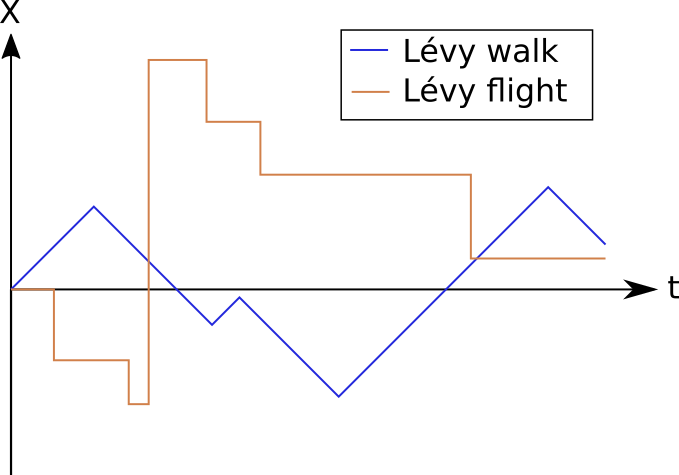
\includegraphics[width=90mm]{pics/levyFlight.png}
\caption{Comparison between the trajectories of the one dimensional L\'evy flight and L\'evy walk (for $\nu=1$). Note that the jump length of the L\'evy flight is independent of the waiting time. 
\label{fig:levyFlight}}
\end{center}
\end{figure}
%
However the L\'evy flight model has a major drawback: Since the jumps happen instantaneously it has an infinite propagation speed, which causes its \gls{msd} and all higher moments to diverge \cite{lwreview}. \\


Therefore the L\'evy walk model was developed by Shlesinger, Klafter and West \cite{shlesinger1987}. Here the walker no longer waits at the change points, but his jumps now have a finite duration, change them into steps. The step duration is coupled to the length of the step and prevents the infinite propagation speed that caused problems with the L\'evy flights, which is illustrated in Fig. \ref{fig:levyFlight}. \\

The path of a walker in the new model is now described by a series of step durations $\gls{dur}_1, \gls{dur}_2, ...$ which are drawn from the power-law distribution 

\begin{align}
\gls{psi}(\gls{dur}_i) = \frac{\gamma}{t_0} \frac{1}{(1+\gls{dur}_i/t_0)^{\gamma+1}} .
\label{eqn:defPsiT}
\end{align}
%
Here the parameter $\gamma>0$ governs the width of the distribution and { \color{red}$t_0$ is the timescale of a step }. These step durations are associated with their respective steps vectors $\ve{x}_1, \ve{x}_2, ...$, whose direction is chosen randomly. By partially summing up the step durations and the step lengths one obtains the change times $\gls{ttime}_n$ and the change points $\gls{tpoint}_n$ respectively:

\begin{align}
\gls{ttime}_n = \sum_{j=1}^n \gls{dur}_j , \qquad \gls{tpoint} = \sum_{j=1}^n \ve{x}_j
\end{align}
%
The walker is now being observed at the observation time $t$: Let the last change time before $t$ be $\gls{ttime}_n = \text{ max} \{\gls{ttime}_i | \gls{ttime}_i \leq t \}$, then the distance covered from the last change point is given by

\begin{align}
\abs{\ve{x}_{n+1}} = c (\gls{dur}_{n+1})^{\nu-1} (t-\gls{ttime}_n) ,
\end{align}
%
where c is a constant with dimension $ [ s t^{-\nu} ] $ . The speed 

\begin{align}
\gls{speed} = \pder{}{t} \abs{\ve{x}_{n+1}} = c (\gls{dur}_{n+1})^{\nu-1}
\end{align}
%
is therefore constant during the entire step but depends on the step duration $\gls{dur}_{n+1}$, where the parameter $\nu>0$ governs this dependence. \\
For any completed step we can now write down the joint probability to make a step of length $\abs{\ve{x}}$ and duration $\gls{dur}$:

\begin{align}
\gls{psi}(\ve{x}, \gls{dur} ) = \frac{\gamma}{t_0} \frac{1}{(1+\gls{dur}/t_0)^{\gamma+1}}  \frac{\delta(\abs{\ve{x}} - c \gls{dur}^{\nu}) }{\abs{\gls{step}}^{d-1} \abs{S^{d-1}}}  \label{eqn:defPsiXT}.
\end{align}
%
Here $d$ is the spatial dimension of the process and $\abs{S^{d-1}}$ is the surface area of a d-dimensional unit ball. Note that both the step duration distribution and the joint distribution are denoted by $\gls{psi}$, but their arguments are different. \\
In conclusion we have a model that is governed by two parameters, $\nu$ and $\gamma$ and can produce different kinds of anomalous diffusion.\\

Because of this versatility the L\'evy walk model is used to describe a variety of systems: Besides the application in turbulent systems for which the model was originally invented it finds application in field like biology, where  the special case of fixed velocities ($\nu=1$) is used to approximate the motion of E. coli bacteria, who move with the help of microscopic flagella. These flagella either rotate in a synchronized manner, which leads to long stretches of relatively fast movement, or unsynchronized, which leads to a tumbling motion in which the bacterium changes its direction. The resulting motion was found to follow a power-law distribution with parameter $\gamma = 1.2$ \cite{korobkova2004}

\todo{more examples: light scattering, chaotic Hamiltonian systems}



However it was found recently in \cite{radons2018} that the \gls{msd} of the model is actually divergent for certain values of its parameters, a fact that had previously gone unnoticed for the three decades of the models existence. 
The divergence can be seen directly when one writes down the contribution to the second moment of the distribution from the trajectories, that consist only of a single step longer than the observation, i.e. where the particle never stops:

\begin{align}
\mean{\ve{x}^2}(t) \geq& \int_{\mathbb{R}^d} \int_{t}^{\infty} \abs{\gls{step}}^{2}(t') \gls{psi}(\gls{step},t') dt' d^{d}x \\
=& \frac{\gamma}{t_0} \int_{0}^{\infty} \int_{t}^{\infty} \abs{\gls{step}}^{2}(t')  \frac{1}{(1+t'/t_0)^{\gamma+1}}  \delta(\abs{\gls{step}} - c (t')^{\nu-1}t)  dt' d\abs{\gls{step}} \\
=& \frac{\gamma t^2}{t_0}  \int_{t}^{\infty}   \frac{c^2 (t')^{2\nu-2}}{(1+t'/t_0)^{\gamma+1}}    dt'  .
\end{align}
%
The integrand is proportional to $(t')^{2\nu-\gamma-3}$, therefore the integral will diverge at infinity whenever $2 \nu \geq \gamma +2$ holds. This includes the parameter region where the Richardson regime was expected, so the model that was essentially invented to cure the divergence in the description of the Richardson regime turns out to be divergent itself. In order to remedy this, a more general model model is necessary.

\todo{Say something about ballistic cone?}

\subsection{Generalized L\'evy walks}

Because the divergence of the second moment is caused by very long steps that result in arbitrarily high velocities throughout the entire step, a solution can be found by letting the particle start with a lower initial speed and compensating for the slower start by accelerating it throughout the step, so that it catches up with its constant velocity counterpart at the end of the step. \\
There are indeed some models that describe particles under acceleration \cite{schulz1997, BarkaiKlafterBuch} that are similar to the Drude model for solids. There it is shown that the MSD exists in the regime where one would expect the Richardson law. \\
Furthermore in the supplementary material of \cite{radons2018} a model is presented that introduces an additional parameter, $\eta$, that allows one to interpolate between the original L\'evy model and the Drude like sheme. It is this model, which I will call generalized L\'evy walk model, that I will investigate in this thesis. \\

The generalized model uses the same distribution of step durations as the previous model (\ref{eqn:defPsiT}), but the position between two change points is calculated differently. Instead of a linear time dependence we now have a dependence on the new parameter $\eta$ for the displacement in the (n+1)th step:
%
\begin{align}
\abs{\ve{x}_{n+1}} = c (\gls{dur}_{n+1})^{\nu-\eta} (t-\gls{ttime}_n)^{\eta} .
\end{align}
%
Therefore the particle moves in general with a non-constant speed  
%
\begin{align}
\gls{speed} = c \eta (\gls{dur}_{n+1})^{\nu-\eta} (t-\gls{ttime}_n)^{\eta-1} .
\end{align}

We note, that this changes neither the change points, nor the change times and the distribution of completed steps is still given by 

\begin{align}
\gls{psi}(\ve{x}, \gls{dur} ) = \frac{\gamma}{t_0} \frac{1}{(1+\gls{dur}/t_0)^{\gamma+1}}  \frac{\delta(\abs{\ve{x}} - c \gls{dur}^{\nu}) }{\abs{\gls{step}}^{d-1} \abs{S^{d-1}}}  .
\end{align}


\begin{figure}
\begin{center}
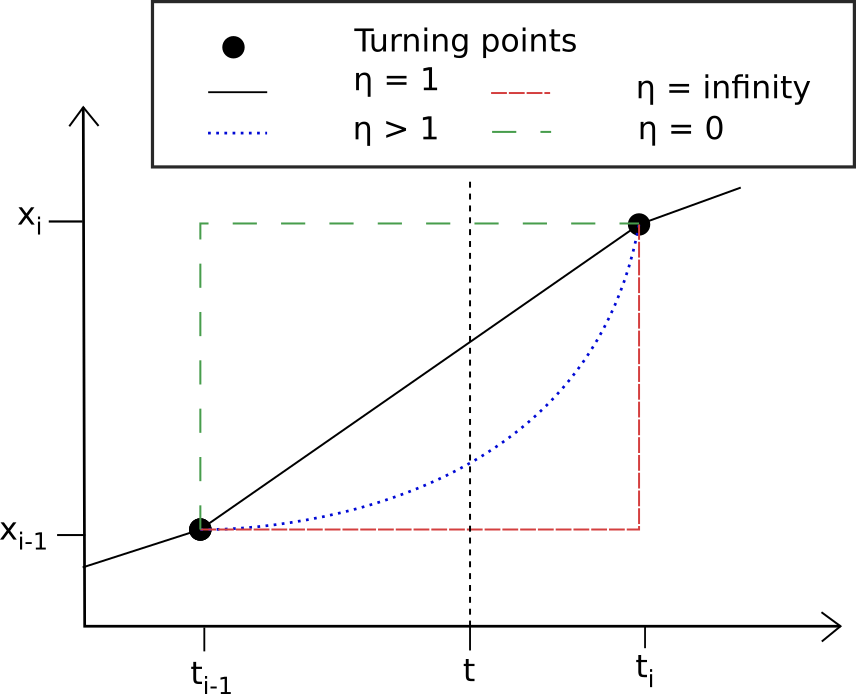
\includegraphics[width=90mm]{pics/turningPoints.png}
\caption{Comparison of the walkers motion for different values of $\eta$: The trajectories and change points remain the same, but the position measured at time $t$ varies. For $\eta = 1$ the walker moves with constant speed and has some non-linear time dependence for $\eta > 1$. In the limits $\eta = 0$ and $\eta = \infty$ we replicate the time-coupled L\'evy flight, where the two limits correspond to the walker jumping first and the then waiting or waiting first and then jumping. 
\label{fig:turningPoints}}
\end{center}
\end{figure}

However as is pointed out in the supplementary material of \cite{radons2018} the position in between two change times now depends on $\eta$, which is  illustrated in Fig. \ref{fig:turningPoints}. This affects the last incomplete steps of the walk, which we have seen to be responsible for the divergence in the original model. \\
To summarize, the generalized model now depends on three parameters: $\nu$ determines how the step length of the walker depends on the step durations, $\eta$ governs the acceleration in between the change points and $\gamma$ describes the width of the waiting time distribution. \\

{\color{blue}
To understand the reason for the anomalous nature of L\'evy walk diffusion we have to look at the moments of the steps: We can directly read off from Eq. (\ref{eqn:defPsiT}) that the mean step duration is only finite for $\gamma<1$. Furthermore we consider the distribution of lengths of completed steps, which follows from Eq. (\ref{eqn:defPsiT}) by using $\abs{\ve{x}} = c t^{\nu}$ which results in
%
\begin{align}
p(\abs{\ve{x}}) dx \propto \abs{\ve{x}}^{-\frac{\gamma+\nu}{\nu}} dx .
\end{align}
%
From this we can deduce that the mean squared step length is only finite for $2\nu < \gamma$. This is of great importance because the central limit theorem asserts that the cumulative distribution of the sum of $N$ independent identically distributed random variables of finite variance tends towards a Gaussian as $N \to \infty$. This applies to the L\'evy walk only when the mean squared step length is finite and the number of steps actually tends to infinity, i.e. when the mean step duration does not diverge. In other words, for $\gamma > 2 \nu$, $\gamma >1$ we expect the \gls{PDF} of the walk to tend towards a Gaussian in the asymptotic limit where it should show normal diffusive behavior $\mean{\ve{x}^2} \propto t$. \\
However outside these parameter ranges the walk is no longer subject to the central limit theorem. Instead it was shown by Paul L\'evy in 1920 that in this case the distribution of the sum of the variables converges to one of the so called L\'evy alpha stable distributions, which  is the statement of the generalized central limit theorem \cite{lwreview}.  

\todo{get first hand source(s) for this}
It is this close relation to L\'evy distributions that gave the L\'evy flights and later the L\'evy walks their name. The divergence of the step length is therefore not bug, but a key feature for the modeling of anomalous diffusion. \\  

A second important quality of the L\'evy walk model in general and the generalized model in particular is that it is a semi-Markov process. A process is considered Markov if the behavior of the walker after a point in time $t_0$ only depends on its position and velocity at $t_0$, not on its history. For a \gls{ctrw}, of which L\'evy walks are an example, this is usually not the case, as information about the last step, i.e. how long the walker is already moving, is important for predicting the future behavior (with the exception of Gaussian step distributions). However in our case this memory only extends to the last previous step, and the process is renewed at every change point, therefore it is semi-Markov \cite{lwreview}.\todo{first hand source} \\
Since the path of the walker is dependent on its behavior prior to the beginning of observation it is of great interest to capture this dependence through suitable initial distributions. This was investigated for similar models in \cite{barkai2003a, barkai2003b} and in this thesis the distribution of the first change point $\gls{first}(x,t|t_a)$ conditioned on the process aging for a time $t_a$ is of major importance, as it is needed to calculate the \gls{msd} of the aged walk.\\

A third related property is weak ergodicity breaking in \gls{ctrw}s. A process breaks ergodicity if its time averages and ensemble averages do not converge to the same values, usually because the trajectory of the solution observed in the time average can not reach the entire phase space, thus giving it only a partial sample. However in the case of weak ergodicity breaking the particle is able to reach the entire phase space, but the time to do this is on the same scale or larger then the total observation time, which means it does not converge reliably to the same value. \\
Ergodicity breaking is of great interest for the theoretical as well as the experimental community as it determines what results we can expect from different kinds of measurements. Power law distributions as used in L\'evy process are closely connected to weak ergodicity breaking, as their typical timescale for reaching a convergent average is divergent in subdiffusive regimes \cite{anomalousTransport}, which has been studied for example in \cite{brokmann2003,radons2018}.\\
While this thesis will not investigate the ergodicity breaking of the new model explicitly, this property is connected to the aged behavior of the walk, which is derived for the MSD. \\
}
Also note that all averages throughout the thesis are understood to be ensemble averages.
\todo{mention further generalizations of the model}
% Further generalizations of the model

\section{Theory of random walks} \label{sec:theory}
 
In this chapter I will briefly cover some of the main results of the theory of random walks that are used in this thesis. A more detailed description can be found in \cite{firstSteps}.


\subsection{Continuous time random walks}
% zoom in from RW -> CTRW -> space-time coupled CTRWs

\subsubsection{Mean number of steps}

The mean number of steps taken in a walk, $\gls{stepNumber}(t)$, gives an estimate for how fast a walker reaches the regime of asymptotic behavior that is calculated in this thesis and is therefore important for the comparison of analytical results with numerical simulations.\\
To derive a general expression for $\gls{stepNumber}(t)$ it is necessary to introduce three auxiliary quantities: The survival probability $\gls{surv}(t)$ describes the chance of a time stretch to last longer than $t$ and can be written as
%
\begin{align}
\gls{surv}(t) = \int_{t}^{\infty} \gls{psi}(t') dt' ,
\end{align}
%
where $\gls{psi}(t)$ is the distribution of time stretches. The Laplace transform of such an integral is known and results in 
%
\begin{align}
\gls{surv}(s) = \frac{1-\gls{psi}(s)}{s} \label{eqn:surv}.
\end{align}

Additionally we need the probability of starting the n-th step at time $t$, denoted by $\gls{nthStepStart}_{n}(t)$. It obeys the recursion relation
%
\begin{align}
\gls{nthStepStart}_{n}(t) = \int_{0}^{t} \psi_{n-1}(t') \gls{psi}(t-t') dt' ,
\end{align}
%
Using the convolution property of the Laplace transform (\ref{eqn:LConvolution}) and induction we find in the Laplace domain:
%
\begin{align}
\gls{nthStepStart}_n(s) = \gls{psi}^{n}(s) \label{eqn:nthStepStart}.
\end{align}

These two quantities allow us to write down the probability of being in the n-th step at time $t$, $\gls{nthStep}(t)$, i.e. the probability of having started the n-th step at time $t'$ and this step lasting longer than $t-t'$:
%
\begin{align}
\gls{nthStep}_n(t) = \int_{0}^{t} \gls{nthStepStart}_{n}(t') \gls{surv}(t-t') dt' .
\end{align}
%
Going into the Laplace domain and using results (\ref{eqn:surv}) and (\ref{eqn:nthStepStart}) we arrive at 
%
\begin{align}
\gls{nthStep}_n(s) =  \gls{nthStepStart}_{n}(s) \gls{surv}(s) = \gls{psi}^{n}(s)  \frac{1-\gls{psi}(s)}{s} .
\end{align}

The desired mean number of steps can now be expressed as the sum over the $\gls{nthStep}_n$:
%
\begin{align}
\gls{stepNumber}(t) = \sum_{n=0}^{\infty} n \gls{nthStep}_n(t) ,
\end{align}
%
which yields a closed expression in the Laplace domain:
%
\todo{see how it depends on existence of first moment}

\begin{align}
\gls{stepNumber}(s) & = \frac{1-\gls{psi}(s)}{s} \sum_{n=0}^{\infty} n \gls{psi}^{n}(s) \\
& =  \frac{\gls{psi}(s)}{s(1-\gls{psi}(s))} .
\end{align}


% introduce: survival probability, forward waiting time, step rate, mean number of steps 

% derive formula for number of steps 

% derive formula waiting times

\subsection{Space-time coupled continuous time random walks}

\todo{smooth introduction from previous chapter}

For a space-time coupled \gls{ctrw} such as the L\'evy walk a each step is determined by a joint distribution of both the step duration $\gls{dur}$ and the step distance $\gls{step}$, where the coupling between space and time is introduced by one being conditioned on the other:

\begin{align}
\gls{psi}(\gls{step}, \gls{dur}) = \gls{psi}(t) f(\gls{step}|t) .
\end{align}

We are now interested in the distribution of completed steps $\gls{comp}(x,t)$, which is the probability density that a particle starting at $\ve{x}=0$, $t=0$ reaches a change point at time $t$ and position $\ve{x}$ after an arbitrary number of steps in between. \\
A transport equation can be written down for $\gls{comp}(x,t)$ \cite{firstSteps}, which reads

\begin{align}
\gls{comp}(\ve{x},t) = \int_{-\infty}^{\infty} d^{d}\ve{x}' \int_{0}^{t} dt' \gls{comp}(\ve{x}',t')  \; \psi(\ve{x}-\ve{x}',t-t') + \delta(t) \delta(\ve{x}) . \label{eqn:CTransport}
\end{align}
%
The two terms on the right hand side express two different contributions to the probability of finding a change point at $(t,\ve{x})$: The first term is a convolution integral in $\ve{x'}$ and $t'$. It expresses the tautology that there will be a change point at $(\ve{x},t)$ exactly when there has been a change point at the primed coordinates $(\ve{x'},t')$ and the particle performed a jump with displacement $\ve{x}-\ve{x}'$ and duration $t-t'$ from $(\ve{x'},t')$ to $(\ve{x},t)$.  \\
The second term just enforces that by definition of the density we will find the particle at the origin at the beginning of observation. \\
To evaluate this integral equation it is useful to go to the Fourier Laplace domain, where the transformations are defined as follows:

The Laplace transform of a function $f(t)$ is defined as the integral 

\begin{align}
\mathcal{L} \left\{ f(t), s \right\} = f(s) = \int^{\infty}_{0} e^{-st} f(t) dt .
\end{align}
%
Note that the distinction between the function and its transform is only made in the argument of the function, which is either $t$ or $s$. \\
The Laplace transform is unique up to a set of points with Lebesgue measure zero and can be inverted via the Bromwich integral 
%
\begin{align}
\mathcal{L}^{-1} \left\{ f(s), t \right\} = f(t) = \frac{1}{2 \pi i} \int^{+i \infty + c}_{-i \infty + c} e^{st} f(s) ds, 
\end{align}
%
where $c \in \mathbb{R}$ is chosen such that $f(s)$ exists on the contour. 
\todo{move this to the first place I am using it}

For Fourier transforms I use the variables $\ve{x} \leftrightarrow \ve{k}$, with the distinction between the function and its transform being made only via the argument. It is defined as 
%
\begin{align}
\mathcal{F} \left\{ f(\ve{x}), \ve{k} \right\} = f(\ve{k}) = \int_{\mathbb{R}^{d}} e^{i\ve{k} \cdot \ve{x}} f(\ve{x}) d^{d}x ,
\end{align}
%
with inverse 
%
\begin{align}
\mathcal{F}^{-1} \left\{ f(\ve{k}), \ve{x} \right\} = f(\ve{x}) = \frac{1}{2 \pi} \int_{\mathbb{R}^{d}} e^{-i\ve{k} \cdot \ve{x}} f(\ve{k}) d^{d}k ,
\end{align}
%
where the normalization factor $\frac{1}{2 \pi}$ is kept in the inverse transform.\\

A useful property of the Fourier and the Laplace transform is that they turn convolutions of functions into simple products. In particular:
%
\begin{align}
\mathcal{L} \left\{ \int_{0}^{t} f(t') g(t-t') dt', s \right\} = f(s) g(s) , \label{eqn:LConvolution}
\end{align}
%
and 
%
\begin{align}
\mathcal{F} \left\{ \int_{\mathbb{R}^{d}} f(\ve{x}') g(\ve{x} - \ve{x}') d^{d}x' , \ve{k} \right\} = f(\ve{k}) g(\ve{k})  \label{eqn:FConvolution} .
\end{align}

Applying this to the integral equation \ref{eqn:CTransport} we obtain 

\begin{align}
\gls{comp}(\ve{k},s) =  \gls{comp}(\ve{k},s)  \; \psi(\ve{k},s) + 1 ,
\end{align}
%
and therefore 
%
\begin{align}
\gls{comp}(\ve{k},s) = \frac{1}{1 - \psi(\ve{k},s)} \label{eqn:CFourierLaplace} .
\end{align}

Our next goal is to use this result to write down an expression for the probability distribution of the ordinary, meaning non-aged, L\'evy walk $\gls{pdf}(\ve{x}|t)$. It describes the probability of finding the walker at $\ve{x}$ given that it is observed at time $t$, where it can either be at a change point or in motion, as illustrated in Fig. \ref{fig:pdfOrdinary}. 

\begin{figure}
\begin{center}
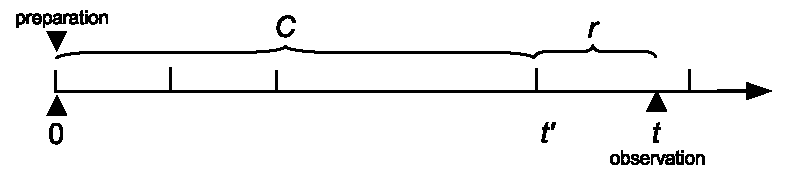
\includegraphics[width=90mm]{pics/timelineOrdinary.png}
\caption{Illustration of the path of a L\'evy walker on the time axis. Each tick on the line represents a change time. The walker starts at $t=0$ and is observed at time $t$ during a final incomplete step described by the distribution $\gls{rest}(\ve{x},t)$ after it has completed a series of steps, which is described by $\gls{comp}(\ve{x},t)$. 
\label{fig:pdfOrdinary}}
\end{center}
\end{figure}

In order to write down a transport equation for $\gls{pdf}(\ve{x}|t)$ we need to introduce the probability density for the rest of the walk after the last change point, denoted by $\gls{rest}(\ve{x}|t)$
\footnote{
Throughout the thesis I will use capital letters for probability densities that depend jointly on space and time, like $\gls{comp}(\ve{x},t)$ and lower case letters for densities that depend only on space and are conditioned on time, like $\gls{rest}(\ve{x}|t)$. Note that the former have dimension $[L^{-d} t^{-1}]$, while the latter have dimension $[L_{-d}]$.
}. 
As shown in Fig. \ref{fig:pdfOrdinary} $\gls{rest}(\ve{x}|t)$ describes the probability of the walker being displaced by the vector $\ve{x}$ after a given time $t$ during a step whose total duration is larger or equal to $t$:\\
%
{ \color{blue}
\begin{align}
\gls{rest}(\ve{x}|t) = \delta(\ve{x} - \ve{x}'(t'=t)) \int_{t}^{\infty} \gls{psi}(\ve{x}',t') dt' .
\end{align}
}
%
\\

With this expression for $\gls{rest}(\ve{x}|t)$ we can now write down $\gls{pdf}(\ve{x}|t)$ as a convolution of $\gls{rest}(\ve{x}|t)$ and $\gls{comp}(\ve{x},t)$
%
\begin{align}
\gls{pdf}(\ve{x}|t) = \int_{\mathbb{R}^{d}} \int_0^t  \gls{comp}(\ve{x}',t') \gls{rest}(\ve{x}-\ve{x}'|t-t') d t' d^{d}x' ,
\end{align}
%
which describes the particle starting at the origin, performing a series of completed steps ending at $\ve{x'}$ and then performing a final, incomplete step that leaves it at position $\ve{x}$ at observation time $t$.\\
We now use the convolution properties of the Fourier and the Laplace transform, equations (\ref{eqn:FConvolution}) and (\ref{eqn:LConvolution}), to obtain 
%
\begin{align}
\gls{pdf}(\ve{k}|s) = \gls{comp}(\ve{k},s) \gls{rest}(\ve{k}|s) \label{eqn:pdfFourierLaplaceI} .
\end{align}
%
Substituting for $\gls{comp}(\ve{k},s)$ with formula (\ref{eqn:CFourierLaplace}) yields
%
\begin{align}
\gls{pdf}(\ve{k}|s) = \frac{ \gls{rest}(\ve{k}|s)}{1 - \gls{psi}(\ve{k},s)} \label{eqn:pdfFourierLaplaceII} ,
\end{align}
%
which gives us an algebraic equation for the \gls{PDF} in the Fourier Laplace domain, that depends only on the the transforms of the step probability density and its time integral. This is a key result for the treatment of space-time coupled \gls{ctrw} {\color{blue} and will be useful for the analytical investigation into the \gls{PDF} later on.} \\

\begin{figure}
\begin{center}
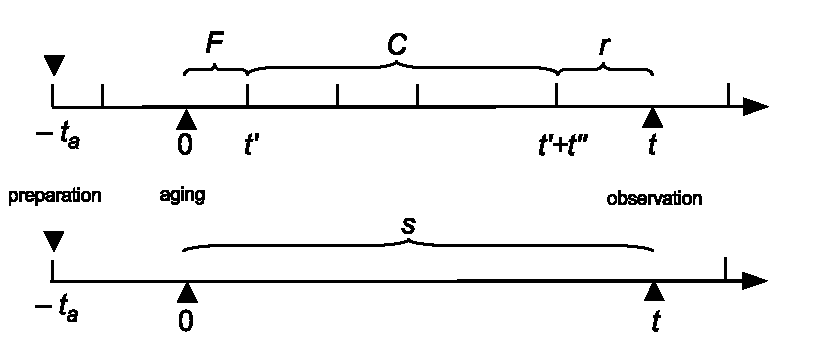
\includegraphics[width=90mm]{pics/timelineAged.png}
\caption{Illustration of an aged L\'evy walk on the time axis. Each tick on the line represents a change time. The walker starts at $-t_a$ and observation begins at $t=0$.  The upper picture shows the case where the first change time $t'$ is smaller than the observation time $t$, described by $\gls{first}$. From here it performs a series of completed steps and a final incomplete step as in the ordinary case. The lower picture shows the case that the first change point is after the end of observation, i.e. the walker never turns during observation. The probability density of this event is given by $\gls{single}$.
\label{fig:pdfAged}}
\end{center}
\end{figure}

A slightly more complicated approach is needed when aging effects are considered. In this case the walker has already moved for the duration of the aging time $t_a$ before the observation begins, which is illustrated in Fig. \ref{fig:pdfAged}. \\
At the beginning of observation, which is set to $t=0$ and $\ve{x}=0$, the walker will already be in motion and has its first observed change point some time after the beginning of observation, where we denote the probability of this change point being at $\ve{x'}$ at time $t'$ with $\gls{first}(\ve{x}',t'|t_a)$. \\
Alternatively the walker can also perform a step so long that it stays in straight motion for the entire duration of observation. In this case  no first change point is observed and this event of a long, single step is instead described by $s(\ve{x}|t,t_a)$, which is the conditional probability that a walker that has aged for $t_a$ performs a step of duration longer than $t$ such that he is at $\ve{x}$ at time $t$. \\

The transport equation for the \gls{PDF} therefore has two terms corresponding to these cases:
%
\begin{align}
\gls{pdf}(\ve{x}|t,t_a) = &\int_{\mathbb{R}^d} d^{d}x' \int_{\mathbb{R}^d} d^{d}x'' \int_{0}^{t} dt' \int_{0}^{t-t'} d t''   F(\ve{x}',t'|t_a)  \gls{comp}(\ve{x}'',t'') \gls{rest}(\ve{x}-\ve{x}'-\ve{x}''| t-t'-t'') \nonumber \\
&+ s(\ve{x}|t,t_a).
\end{align}
%
The second term captures the contribution from the single step case while the double convolution describes a particle having its first change point at $t'$, then performing a series of completed steps for the duration $t''$ and then being found at observation time $t$ in a final, incomplete step of duration $t-t'-t''$ or longer, as shown in the upper picture of Fig. \ref{fig:pdfAged}.\\
Again using the convolution property of the Fourier and the Laplace transform,  (\ref{eqn:FConvolution}) and (\ref{eqn:FConvolution}), we obtain the a closed expression for $\gls{pdf}(\ve{k}|s,t_a)$:
%
\begin{align}
\gls{pdf}(\ve{k}|s,t_a) =  \gls{first}(\ve{k},s|t_a)  \gls{comp}(\ve{k},s) \gls{rest}(\ve{k}|s) + s(\ve{k}|s,t_a) \label{eqn:pdfAgedFourierLaplace}.
\end{align}


\paragraph{Forward waiting time}

Consider a walker in a \gls{ctrw} that has aged for a time $t_a$. When the observation begins the walker will in general not be at a change point, but rather in some time interval that started before the beginning of observation. To describe this we use the forward waiting time $\gls{forwardWaiting}(t|t_a)$, which gives the probability density that the first change time after the beginning of observation is $t$ when the aging time of the walk is $t_a$. \\

In order to derive a formula for $\gls{forwardWaiting}(t|t_a)$ consider a walker starting at time zero, then performing exactly n steps that that end at $t' < t_a$ and then taking a final step of duration $t_a-t'+t$, i.e. a walker whose first change point during the observation beginning at $t_a$ is exactly at $t$. The probability density of this event is given by
%
\begin{align}
\gls{forwardWaitingNSteps}_n(t|t_a) = \int^{t_a}_{0} \gls{nthStepStart}_n(t') \gls{psi}(t_a-t'+t) dt'.
\end{align}
%
To obtain the forward waiting time we need to sum over all possible numbers of steps 
%
\begin{align}
\gls{forwardWaiting}(t|t_a) = \sum_{n=0}^{\infty} \gls{forwardWaitingNSteps}_n(t|t_a) 
= \int^{t_a}_{0} \left( \sum_{n=0}^{\infty}  \gls{nthStepStart}_n(t') \right) \gls{psi}(t_a-t'+t) dt',
\end{align}
%
which can be expressed via the step rate
%
\begin{align}
\gls{stepRate}(t) =  \sum_{n=0}^{\infty}  \gls{nthStepStart}_n(t')  \label{eqn:stepRate},
\end{align}
%
as 
%
\begin{align}
\gls{forwardWaiting}(t|t_a) = \int^{t_a}_{0} \gls{stepRate}(t') \gls{psi}(t_a-t'+t) dt'.
\end{align}

For future calculations it is useful to note that $\gls{stepRate}(t)$ has a simple form in the Laplace domain,
%
\begin{align}
\gls{stepRate}(s) = \frac{1}{1-\gls{psi}(s)} ,
\end{align}
%
which follows directly from the factorization of $\gls{nthStepStart}_n$ in (\ref{eqn:nthStepStart}).\\

In the case of a power law time distribution that lacks the first moment, e.g. the distribution for the generalized L\'evy walk (\ref{eqn:defPsiT}) with $\gamma < 1$, the forward waiting time can be calculated exactly and reads \cite{firstSteps}:
%
\begin{align}
\gls{forwardWaiting} = \frac{\sin(\pi \gamma)}{\pi} \left( \frac{t_a}{t} \right)^{\gamma} \frac{1}{t+t_a} \label{eqn:forwardWaiting} .
\end{align}

 %Theoretical Background
\chapter{Methods}

\section{Method for calculating the MSD} 

For the calculation of asymptotic behavior of the \gls*{msd} we concentrate on the one-dimensional case, as this simplifies the calculations. The generalization to higher dimensions is straightforward, because the \gls*{PDF} of the process, Eq. (\ref{eqn:defPsiXT}), is isotropic and the normalization takes care of the angular integration. 

The one-dimensional \gls*{msd} $\mean{x^2}(t)$ is defined via the integral 
%
\begin{align}
\mean{x^2}(t) = \int_{\mathbb{R}} x^2 \gls*{psi}(x,t) dx ,
\end{align}
%
which is closely related to the Fourier-Laplace transform of the \gls*{PDF} for the process, as we can see when we expand it for small $k$:
%
\begin{align}
\gls*{pdf}(k|s) &= \int_{\mathbb{R}}  e^{ik x} p(x|s) dx  \\
&= \int_{\mathbb{R}}   p(x|s) dx +  i k \int_{\mathbb{R}}   x p(x|s) dx - \frac{k^2}{2} \int_{\mathbb{R}}   x^2 p(x|s) dx \\
&= 1 - \frac{k^2}{2} \mean{x^2}(s)  + ... \quad ,
\end{align}
%
where we used that the \gls*{PDF} is normalized to one and that the first moment of an isotropic process vanishes. This implies 
%
\begin{align}
\mean{x^2}(s) = - \left[ \npder{}{k}{2} \gls*{pdf}(k|s) \right]_{k=0} \label{eqn:MSDDerivative}, 
\end{align}
%
which allows us to calculate the \gls*{msd} directly without knowledge of the full \gls*{PDF}.

For the ordinary case we can use Eq. (\ref{eqn:pdfFourierLaplaceI}) for the \gls*{PDF} in the Fourier-Laplace domain:
%
\begin{align}
\gls*{pdf}(k|s) = \gls*{comp}(k,s) \gls*{rest}(k|s) \label{eqn:PDFFourierLaplaceMethods} .
\end{align}
%
We now expand $\gls*{comp}$ and $\gls*{rest}$ similarly to what we did for the \gls*{PDF}, resulting in in 
%
\begin{align}
\gls*{rest}(k|s) &= \gls*{rest}_0(s) - \frac{1}{2} k^2 \gls*{rest}_2(s) + o(k^2) \label{eqn:rExpansion} ,\\
\gls*{comp}(k,s) &= \gls*{comp}_0(s)- \frac{1}{2} k^2 \gls*{comp}_2(s) + o(k^2) .
\end{align}
%
Here the first moments vanish again and we introduced the following notation for the marginal moments:
%
\begin{align}
\gls*{rest}_0(s) &=   \gls*{rest}(k=0|s), \qquad \gls*{rest}_2 (s) =   \left[ \npder{}{k}{2} \gls*{rest}(k|s) \right]_{k=0}, \\
\gls*{comp}_0(s) &=   \gls*{comp}(k=0|s), \qquad \gls*{comp}_2 (s) =   \left[ \npder{}{k}{2} \gls*{comp}(k|s) \right]_{k=0}.
\end{align}
%
Inserting these expansions into Eq. (\ref{eqn:PDFFourierLaplaceMethods}) we find for the \gls*{PDF}
%
\begin{align}
\gls*{pdf}(k|s)  = \gls*{comp}_0(s)\gls*{rest}_0(s) - \frac{k^2}{2}\left[\gls*{comp}_0(s) \gls*{rest}_2(s)+\gls*{comp}_2(s)\gls*{rest}_0(s)\right] +o(k^2) ,
\end{align}
%
from which it follows by Eq. (\ref{eqn:MSDDerivative}) that in the ordinary case the \gls*{msd} is given by 
%
\begin{align}
\mean{x^2}(s) = \gls*{comp}_0(s) \gls*{rest}_2(s)+\gls*{comp}_2(s)\gls*{rest}_0(s) \label{eqn:x2Ordinary}. 
\end{align}
%
For the aged case we start from the result found in Eq. (\ref{eqn:pdfAgedFourierLaplace}),
%
\begin{align}
\gls*{pdf}(k|s,t_a) =  \gls*{first}(k,s|t_a)  \gls*{comp}(k,s) \gls*{rest}(k|s) + \gls*{single}(k|s,t_a) ,
\end{align}
%
and use a similar expansions for the transforms of the single step density and the first step density:
%
\begin{align}
\gls*{single}(k|s,t_a) &= \gls*{single}_0(s,t_a) - \frac{1}{2} k^2 \gls*{single}_2 (s,t_a) + o(k^2) ,\\ 
\gls*{first}(k,s|t_a) &= \gls*{first}_0(s|t_a)- \frac{1}{2} k^2 \gls*{first}_2(s|t_a) + o(k^2) .
\end{align}
%
Thus we find for the \gls*{PDF}
%
\begin{align}
\begin{split}
 p(k|s) = \gls*{first}_0(s|t_a)\gls*{comp}_0(s)\gls*{rest}_0(s) - \frac{k^2}{2} &\left[ \gls*{first}_0(s|t_a)\gls*{comp}_0(s) \gls*{rest}_2(s) +\gls*{first}_0(s|t_a)\gls*{comp}_2(s)\gls*{rest}_0(s)  \right. \\
 & \quad \left. + \gls*{first}_2(s|t_a)\gls*{comp}_0(s) \gls*{rest}_0(s) + \gls*{single}_2(s,t_a)\right] +o(k^2) .
\end{split}
\end{align}
%
Again using Eq. (\ref{eqn:MSDDerivative}) we obtain for the \gls*{msd} in the aged case:
%
\begin{align}
\begin{split}
\mean{x^2}(s) =& \gls*{first}_0(s|t_a)\gls*{comp}_0(s) \gls*{rest}_2(s) +\gls*{first}_0(s|t_a)\gls*{comp}_2(s)\gls*{rest}_0(s)  \\
& + \gls*{first}_2(s|t_a)\gls*{comp}_0(s) \gls*{rest}_0(s) + \gls*{single}_2(s,t_a)  \label{eqn:x2Aged}.
\end{split}
\end{align}

To extract the asymptotic results from Eqs. (\ref{eqn:x2Ordinary}) and (\ref{eqn:x2Aged}) we need to look at the $t \to \infty$ limit, which corresponds to the $s \to 0$ limit in the Laplace domain. \\
The general strategy is therefore to find expressions for the quantities $\gls*{comp}_0, \gls*{first}_0, \gls*{rest}_0, \gls*{comp}_2, \gls*{first}_2, \gls*{rest}_2$ in the Laplace domain to leading order in $s$. They are then inserted into the respective equations for the \gls*{msd}, which is then transformed back into the time domain. $\gls*{single}_2$ can be calculated directly in the time domain, as it is not part of a product in the expression for the aged \gls*{msd}. 

The key tool for moving between the Laplace and the time domain is the Tauberian theorem. It states that the Laplace transform of a function $f(t)$ following a power law for large $t$ through the formula 
\cite{firstSteps}
% 
\begin{equation}
 f(t) \simeq t^{\rho-1} L(t) \;\; \leftrightarrow \;\; f(s) \simeq \Gamma(\rho) s^{-\rho} L\left(\frac{1}{s}\right) \label{eqn:tauberian} ,
\end{equation}
%
if $\rho \geq 0 $ and $L(t)$ is slowly varying, i.e. when
%
\begin{align}
\lim_{t \to \infty} \frac{L(C \; t)}{L(t)} = 1 .
\end{align}
%
For general $\rho$ the slightly more complicated formula 
%
\begin{align}
 f(s) \simeq \sum_{k=0}^{k_{\max}} \frac{(-1)^k}{k!} I^{f}_k s^k + L \Gamma(\rho) s^{-\rho} ,
 \label{eqn:generalTauberian}
\end{align}
%
has to be used, which is derived in Sec. \ref{sec:tauberian}. Here $k_{\max}$ is the whole part of $-\rho$, and $I^{f}_k$ is the moment integral
%
\begin{align}
I^{f}_k = \int_0^\infty t^k f(t) dt.
\end{align}



\section{Method for calculating the PDF}

% great previous work by magdziarz
So far no analytic solution for the \gls*{PDF} of the original L\'evy walk is known for general values of $\gamma$ and $\nu$, which makes finding it for the generalized model a difficult task. However there is a remarkable result by Magdziarz, who found closed expressions for the \gls*{PDF} in any dimension for the special case $\nu=1$ (i.e. the velocity model) 
\cite{magdziarz2015, magdziarz2016}. 
It is therefore tempting to see if his method might be generalized and applied to our case. Unfortunately this turned out to be impossible, as his technique for performing the inverse transform relied heavily on the scaling of the transformed \gls*{PDF}, $\gls*{pdf}(\ve{k}|s) \propto f\left( \frac{k}{s} \right)$, which is not preserved when $\nu$ deviates from 1. In this case the function scales as $\gls*{pdf}(\ve{k}|s) \propto f\left(\frac{k}{s^{\nu}} \right)$ which makes the method unworkable for arbitrary $\nu$.

Instead an asymptotic approach is taken, where the starting point for the calculation is the general expression for the transformed \gls*{PDF} found in  Eq. (\ref{eqn:pdfFourierLaplaceII}):
%
\begin{align}
\gls*{pdf}(\ve{k}|s) = \frac{ \gls*{rest}(\ve{k}|s)}{1 - \gls*{psi}(\ve{k},s)}  .
\end{align}
%
Here an expansion is again performed for the one dimensional PDF, analogously to the calculation of the \gls*{msd}. \\
For the inverse Laplace transform analytical results are supplemented with the use of numerical inverse transforms. These can be performed efficiently through the use of the algorithm proposed by Talbot 
\cite{talbot1979}, 
which has been slightly improved and implemented in Mathematica in 
\cite{abate2004}.


\section{Numerical simulation of the model}

% why use direct simulation
Numerical simulations supplement and support analytical computations by giving insight into the qualitative structure of the process, sharpening the understanding of the model and giving a method of testing the results. Furthermore numerical methods allow the investigation of regimes where no analytical solution can be found.
%{\color{blue}
%In general there are two possible approaches for the simulation of a L\'evy walk model: On the one hand a direct simulation of the process, where I randomly generate step durations and directions for a large ensemble of walkers and record their positions; or on the other hand a description via a suitable Langevin equation, which has been shown to be equivalent to a L\'evy walk. \todo{is it?}
%where  I decided to go with the former approach as it keeps closer to the model and avoids potential numerical instabilities that can appear during the integration of differential equation. It is also not entirely clear how the generalization of the L\'evy walk studied in this paper could be reflected in a Langevin equation. 
%}

The simulation implemented for this thesis creates an ensemble of L\'evy walkers, each of which performing steps whose length and direction is determined by a pseudorandom number generator. Information about the process is then extracted by averaging over the ensemble. 
%Such an approach is very robust compared to the integration of stochastic differential equations, as it does not involve a discretization of time and is therefore very unlikely to run into numerical instabilities. 

The two main quantities that we are interested in for this thesis are the \gls*{msd} and the \gls*{PDF} of the generalized L\'evy walk: The former can be found by computing the position of the walkers at preset measurement times and taking the ensemble averages. For the latter the distance from the origin is split into intervals with bins that track the number of particles in that region. The \gls*{PDF} can then be approximated by plotting the bins in a histogram. This was implemented in one dimension similarly to the analytical computation, as this captures most of the behavior in an isotropic walk. 

The computation time of the simulation depends mainly on the number of steps that have to be computed and the size of the ensemble. As we have seen in the theory section the average number of steps scales with $t^{\gamma}$. This means that the duration of the walk, $t$, is the main parameter for influencing the number of steps. In particular we can choose lower walk durations for simulations with high $\gamma$ values to keep the computation time reasonable.\\
The second limiting factor for performance is the ensemble size, which is of special importance for processes with power law distributions such as L\'evy walks, because these processes are dominated by rare events which are only captured with sufficiently large ensembles. \\
To address this issue I use the independence of the different walkers to parallelize the computation and perform it on the available graphics cards (GPUs) using NVIDIA's C++ extension CUDA. The university computers are equipped with Quadro K4000 GPUs, that have 768 cores each. This is a far greater than the number of cores available on a typical processor (CPU), which is usually less than ten, and thus allows for far greater parallelization, resulting in a theoretical speedup of over $70$. \\
In praxis this is not quite reached, because of the GPU cores being slower individually, the latency in the data transfer between CPU and GPU as well as the smaller memory on the GPU (3GB). However by saving only the sum of squared displacements at selected measurement times and reducing communication between GPU and CPU to a minimum it was possible to simulate large ensembles of $10^9$ walkers in a few hours. 

Another aspect that should be addressed is the generation of pseudorandom numbers for the creation of the steps for the simulation. As these numbers are not truly random, i.e. not completely uncorrelated, they can, depending on the quality of the number generator, leave statistical artifacts that falsify the simulation results. To minimize this risk I use the cuRAND library, which implements a version of the powerful Xorshift algorithm 
\cite{marsaglia2003xorshift}. 
The documentation guarantees a period greater than $2^{190}$ for each independently seeded sequence of random numbers (i.e. each simulation), and each thread has an offset of $2^{67}$ in this sequence. In the simulation no more than $10^{9}$ walkers are used, so we have a total offset of $10^9 \cdot 2^{67}  \simeq 2^{97} << 2^{190}$. In each individual thread the walker performs typically fewer than $10^{7} \simeq 2^{23}$ steps, which is much smaller than the offset of $2^{67}$. The risk that statistical artifacts influence the results is therefore very small.


 %Methodology
\chapter{Analytical Calculations}

\section{Asymptotic behavior of the ordinary MSD}

The calculation of the MSD, both in the ordinary and in the aged case, is taken from \cite{bothe} and presented here again for better understanding of the results:

\subsection*{Calculation of $\gls{psi}_0(s)$}
All properties of the ordinary walk are derived from the waiting time density $\gls{psi}(t)$. The joint probability density of a displacement in a stretch and of the time of stretch is given by
%
\begin{equation}
 \gls{psi}(x,t) = \frac{1}{2} \delta(|x| - ct^\nu ) \gls{psi}(t),
\end{equation}
%
so that the Fourier transform of this function in $x$ reads
\begin{equation}
 \gls{psi}(k,t) = \gls{psi}(t) - \frac{k^2}{2} c^2 t^{2 \nu} \gls{psi}(t) + o(k^2). 
\end{equation}
Then the Laplace transform in $t$ should be performed.  Although the exact Laplace transform of $\gls{psi}(t)$ as given by Eq.(\ref{eqn:defPsiT}) is possible in quadratures, we are only interested in the asymptotic behavior, which can be found using the Tauberian theorem (\ref{eqn:generalTauberian}). The forms of the Laplace transform 
differ for different values of $\gamma$ and $\nu$. As explained above we are interested only in the lowest order terms of $s$-dependence. 

\subsubsection*{$ \gamma<1$}
For $0<\gamma <1$ the function $ \gls{psi}_0(s) = \gls{psi}(s)$ belongs to an integrable class, and its Laplace representation reads
\begin{equation}
 \gls{psi}_0(s) \simeq 1 + \gamma \Gamma(-\gamma) t_0^\gamma s^\gamma 
 = 1-\Gamma(1-\gamma) t_0^\gamma s^\gamma. \label{eqn:psi0GammaSmall}
\end{equation}
Keeping $t_0$ in all calculations and not putting it to unity is reasonable to be able to check the dimension of the ensuing results, especially in the aged case. 

\subsubsection*{$ \gamma>1$}
The Laplace transform of $\gls{psi}(t)$ now has an additional term, due to its first moment being finite:
\begin{equation}
\gls{psi}_{0}(s) \simeq 1 - \tau s - \Gamma(1-\gamma ) t_0^\gamma s^\gamma.
\label{eqn:psi0GammaBig}
\end{equation}  
Here $\tau$ is defined as 
\begin{equation}
 \tau = \frac{\gamma}{t_0} \int_0^\infty \frac{t dt}{(1+t/t_0)^{\gamma +1}} = 
 \frac{t_0}{\gamma-1} . \label{eq:tau}
\end{equation}

\subsection*{Calculation of $\gls{psi}_2(s)$}
The marginal second moment of the step distribution is given by  
\begin{align}
 \gls{psi}_2(t) = \int_{-\infty}^\infty x^2 \gls{psi}(x,t) dx = c^2 t^{2 \nu} \gls{psi}(t).
\end{align}
The expressions for $\gls{psi}_2(s)$ depend on whether $2 \nu < \gamma $ or $2 \nu > \gamma$:

\subsubsection*{$2\nu<\gamma$} 
In this first case the function $\gls{psi}_2(t)$ is integrable, $\int_0^\infty \gls{psi}_2(t) dt < \infty$, and the expansion 
of its Laplace transform starts from a constant:
\begin{equation}
 \gls{psi}_2(s) \simeq \gamma c^2 t_0^{2\nu}  \int_0^\infty \frac{x^{2\nu}}{(1+x)^{\gamma+1}} dx  + \gamma \Gamma(2\nu-\gamma) c^2t_0^\gamma s^{\gamma-2\nu} ,
\end{equation}
where the integral is given by the dimensionless constant 
\begin{equation}
 \int_0^\infty \frac{x^{2\nu}}{(1+x)^{\gamma+1}} dx = \mathrm{B}(2\nu+1,\gamma-2\nu), \label{eqn:I1}
\end{equation}
with $\mathrm{B}(a,b)$ being the Beta-function, which is defined as:
%
\begin{align}
\mathrm{B}(a,b) = \int_{0}^{1} x^{a-1}(1-x)^{b-1} dx = \frac{\Gamma(a)\Gamma(b)}{\Gamma(a+b)} .
\end{align}
%
With this $\gls{psi}_2(s)$ takes the form 
%
\begin{align}
\gls{psi}_2(s) \simeq \gamma c^2 t_0^{2\nu}  \mathrm{B}(2\nu+1,\gamma-2\nu)  + \gamma \Gamma(2\nu-\gamma) c^2t_0^\gamma s^{\gamma-2\nu} \label{eqn:psi2NuSmall} .
\end{align}

\subsubsection*{$2\nu>\gamma$} 
In the second case $\gls{psi}_2(t)$ is non-integrable, the integral $\int_0^\infty \gls{psi}_2(t) dt$ diverges, and the asymptotics of its Laplace transform read
\begin{align}
 \gls{psi}_2(s) \simeq \gamma \Gamma(2\nu-\gamma) c^2  t_0^\gamma s^{\gamma-2\nu}. \label{eqn:psi2NuBig}
\end{align}

\subsection*{Calculation of $\gls{comp}_0(s)$ and $\gls{comp}_2(s)$}

For complete steps our generalization does not differ from the original L\'evy walk and we can use the general result for $\gls{comp}(x,t)$ in the Fourier-Laplace domain Eq. (\ref{eqn:CFourierLaplace}):
%
\begin{align}
\gls{comp}(k,s) = \frac{1}{1 - \gls{psi}(k,s)}.
\end{align}
%
Expanding $\gls{comp}(k,s)$ for $s$ small and in the limit $k \to 0$ we get 
%
\begin{align}
\begin{split}
\gls{comp}(k,s)  &\simeq \frac{1}{1 - \gls{psi}(s) + (k^2/2) \gls{psi}_2(s) +o(k^2)}\\ &\simeq \frac{1}{1-\gls{psi}(s)} - \frac{k^2}{2}  \frac{\gls{psi}_2(s)}{[1-\gls{psi}(s)]^2} + o(k^2).
\end{split}
\end{align}
Therefore 
\begin{align}
\gls{comp}_0(s) =& \frac{1}{1-\gls{psi}(s)}\\
\gls{comp}_2(s) =& \frac{\gls{psi}_2(s)}{[1-\gls{psi}(s)]^2} \;,
\end{align}
into which we now have to insert our results for $\gls{psi}_0$ and $\gls{psi}_2$:

\subsubsection{$\gamma<1$ and $2\nu<\gamma$ }
Here we find by using equations (\ref{eqn:psi0GammaSmall}) and (\ref{eqn:psi2NuSmall}) :
\begin{align}
 \gls{comp}_0(s) \simeq & \frac{1}{\Gamma(1-\gamma)} t_0^{-\gamma} s^{-\gamma}, \label{eq:Co}\\
 \gls{comp}_2(s) \simeq & \gamma   \frac{ \mathrm{B}(2\nu+1,\gamma-2\nu)}{\Gamma^2(1-\gamma)} c^2 t_0^{2\nu - 2\gamma} s^{-2 \gamma} .
\end{align}

\subsubsection{$\gamma<1 \text{ and } 2\nu>\gamma$: }
In this case we obtain for $\gls{comp}_2$:
\begin{equation}
  \gls{comp}_2(s) \simeq  \gamma   \frac{\Gamma(2\nu-\gamma)}{\Gamma^2(1-\gamma)} c^2 t_0^{-\gamma} s^{-2\nu-\gamma},
\end{equation}
while $\gls{comp}_0$ is the same as in Eq.(\ref{eq:Co}) as long as $\gamma<1$.

\subsubsection{$\gamma>1$ and  $2\nu<\gamma$}
Now the first moment of $\gls{psi}(t)$ is finite, therefore 
\begin{align}
 \gls{comp}_0(s) \simeq &  \frac{1}{\tau s}  \\
 \gls{comp}_2(s) \simeq & \gamma \mathrm{B}(2\nu+1,\gamma-2\nu) c^2 \frac{t_0^{2\nu}}{\tau^2}  s^{-2}
\end{align}


\subsubsection{$\gamma>1$ and $2\nu>\gamma$: }
Again $\gls{comp}_0(s)$ doesn't change, and for $\gls{comp}_2$ we obtain
\begin{equation}
\gls{comp}_2 \simeq  \gamma \Gamma(2\nu-\gamma)  c^2 \frac{t_0^\gamma}{\tau^2}   s^{\gamma-2\nu -2} .
\end{equation}

\subsection*{Calculation of  $\gls{rest}_0(s)$ and $\gls{rest}_2(s)$}
The function $\gls{rest}(x|t)$ gives the distribution of
the corresponding displacements conditioned on the fact that the total duration of a stretch is longer than $t$:
\begin{equation}
 \gls{rest}(x|t) =  \int_t^\infty \frac{1}{2} \delta(|x| - c t^{\eta}t'^{\nu-\eta}) \gls{psi}(t') dt' \; .
\end{equation}
This is correctly normalized to the overall probability to stay within a single stretch for a time longer than $t$ 
\begin{equation}
 \int \gls{rest}(x|t)  dx = \int_t^\infty \gls{psi}(t') dt'.
\end{equation}
Expanding the Fourier transform of $\gls{rest}(x,t)$ for small $k$,
\begin{align}
\gls{rest}(k|t) =& \int_{-\infty}^{\infty} dx \; e^{ikx} \int_t^\infty \frac{1}{2} \delta(|x| - c t^{\eta}t'^{\nu-\eta}) \gls{psi}(t') dt' \nonumber \\
=& \gls{rest}_0(t) - \frac{k^2}{2} \gls{rest}_2(t) + o(k^2), 
\end{align}
we find the marginal moments
\begin{align}
\gls{rest}_0(t) =& \frac{1}{(1+t/t_0)^{\gamma}} \\
\gls{rest}_2(t) =& \gamma c^2 \frac{1 }{t_0} t^{2\eta} \int_t^\infty \frac{t'^{2(\nu-\eta)}}{(1+t'/t_0)^{\gamma+1}} dt' \; , 
\end{align}
whose Laplace transforms depend on the relationship between $\gamma$, $\nu$ and $\eta$: 

\subsubsection{$\gamma<1 $ }
In this case $\gls{rest}_0$ is non-integrable and we find
\begin{equation}
  \gls{rest}_0(s) \simeq  \Gamma(1-\gamma) t_0^\gamma s^{\gamma-1}.
\end{equation}
For $\gls{rest}_2$  we can use the asymptotic form of $\gls{psi}(t)$ , since we are interested in large $t$:
\begin{equation}
\gls{rest}_2(t) \simeq \gamma c^2 t_0^\gamma t^{2\eta} \int_t^\infty \tau^{2(\nu-\eta)-1-\gamma}  d\tau   \; , 
\end{equation}
which is only finite for $\gamma > 2(\nu-\eta)$ and diverges otherwise, meaning that no MSD exists. In the rest of 
the paper we will concentrate on the case when the second moment converges, where we find
\begin{equation}
\gls{rest}_{2}(t)  \simeq \gamma\frac{1} {\gamma - 2(\nu-\eta)} c^2 t_0^\gamma t^{2\nu -\gamma}  .
\end{equation}
Since this expression is always in the non-integrable class we obtain by using Tauberian theorem (\ref{eqn:tauberian})
\begin{equation}
\gls{rest}_2(s) \simeq \gamma  \frac{ \Gamma(2\nu+1-\gamma)}{\gamma - 2(\nu-\eta)}c^2 t_0^\gamma s^{\gamma - 2\nu-1}.
\end{equation}

\subsubsection{$\gamma>1$ and $2\nu>\gamma-1$}
For $\gamma>1$ $\gls{rest}_0(t)$ becomes integrable, therefore its Laplace transform reads
\begin{equation}
 \gls{rest}_0 \simeq \tau + \Gamma(1-\gamma) t_0^\gamma s^{\gamma-1} .
\end{equation}
The function $\gls{rest}_2(t)$ is still non-integrable and therefore identical to the previous case.

\subsubsection{$\gamma>1$ and $2\nu<\gamma-1$}
In this case $\gls{rest}_0$ does not change but $\gls{rest}_2(s)$ is now integrable and therefore its transform behaves as
\begin{equation}
\gls{rest}_2(s) \simeq I^{\gls{rest}_2}_0 - \gamma \frac{\Gamma(2\nu+1-\gamma)}{2(\nu-\eta)-\gamma} c^2 t_0^\gamma s^{\gamma - 2\nu-1 } \; .
\end{equation}
We evaluate the definite integral $I^{\gls{rest}_2}_0$ by manipulating the area of integration:
\begin{align}
 I^{\gls{rest}_2}_0 =& c^2\int_0^\infty dt  t^{2\eta} \int_t^\infty dt' \gls{psi}(t') (t')^{2(\nu-\eta)} \\
  =& c^2\frac{1}{2\eta+1} \int_0^\infty \gls{psi}(t') t'^{2\nu+1} dt' \nonumber \\ 
 =& \gamma\frac{1}{2\eta+1} \int_0^\infty \frac{x^{2\nu+1}dx}{(1+x)^{\gamma+1}}c^2 t_0^{2\nu+1}  \nonumber \\
=& \gamma  \frac{\mathrm{B}(2\nu +2, \gamma - 2\nu -1)}{2\eta+1}  c^2 t_0^{2\nu+1} , 
\end{align}
meaning the $\gls{rest}_2$ is constant in the leading order. Therefore we find for $\gamma>1$ and $2\nu<\gamma-1$

\begin{align}
\gls{rest}_2 \simeq & \gamma \frac{\mathrm{B}(2\nu +2, \gamma - 2\nu -1)}{2\eta+1}  c^2 t_0^{2\nu+1}   -\gamma \frac{\Gamma(2\nu+1-\gamma)} {2(\nu-\eta)-\gamma} c^2 t_0^\gamma  s^{\gamma - 2\nu-1} .
\end{align}

The results so far are summarized in Table \ref{tab:Cr}.


\begin{center}
\begin{table}[htb]
 \begin{tabular}{||l|l|l||}
 \hline \hline
 \rule[-4mm]{0cm}{1cm} $\gamma<1$ & 
 $\gls{comp}_0(s) \simeq \frac{1}{\Gamma(1-\gamma)}t_0^{-\gamma} s^{-\gamma}$ & 
 $\gls{comp}_2(s) \simeq \left\{
\begin{array}{ll}
\gamma \frac{\mathrm{B}(2\nu+1,\gamma-2\nu)}{\Gamma^2(1-\gamma)} c^2 t_0^{2\nu - 2\gamma} s^{-2 \gamma} &\mbox{for } 2\nu < \gamma \\
 \gamma \frac{\Gamma(2\nu-\gamma)}{\Gamma^2(1-\gamma)} c^2 t_0^{-\gamma} s^{-2\nu-\gamma} &\mbox{for } 2\nu > \gamma
\end{array} \right. $ \\ \hline
\rule[-4mm]{0cm}{1cm}  $\gamma<1$ &$\gls{rest}_0(s) \simeq \Gamma(1-\gamma)t_0^\gamma s^{\gamma-1}$ & $\gls{rest}_2(s)  \simeq \gamma \frac{\Gamma(2\nu+1-\gamma)}{\gamma- 2(\nu-\eta)}c^2 t_0^\gamma s^{\gamma-1-2\nu}$ \\ \hline
\rule[-4mm]{0cm}{1cm}   $\gamma>1$ & $\gls{comp}_0(s) \simeq   \frac{1}{\tau s}$ & 
 $\gls{comp}_2(s) \simeq \left\{ \begin{array}{ll}
 \gamma \mathrm{B}(2\nu+1,\gamma-2\nu)c^2 \frac{t_0^{2\nu}}{\tau^2}  s^{-2} & \mbox{for } 2\nu < \gamma \\
\gamma \Gamma(2\nu-\gamma)c^2\frac{t_0^\gamma}{\tau^2} s^{\gamma-2\nu -2}  & \mbox{for }  2\nu > \gamma
\end{array} \right. $\\ \hline
\rule[-4mm]{0cm}{1cm} $\gamma>1$ &$\gls{rest}_0(s) \simeq\ \tau$ 
 & $\gls{rest}_2(s) \simeq \left\{ \begin{array}{ll}
\gamma\frac{\mathrm{B}(2\nu +2, \gamma - 2\nu -1)}{2\eta+1}  c^2 t_0^{2\nu+1}  & \mbox{for } 2\nu < \gamma -1 \\
\gamma \frac{\Gamma(2\nu+1-\gamma)}{\gamma - 2(\nu-\eta)}  c^2 t_0^\gamma   s^{\gamma - 2\nu-1}& \mbox{for } 2\nu > \gamma -1 
\end{array} \right.$ \\ \hline \hline
\end{tabular}
\caption{Leading terms of the marginal moments of $C$  and $r$ in the Laplace domain for different parameter ranges. \label{tab:Cr}}
\end{table}
\end{center}



\subsection*{Mean squared displacement}
With these results we can now compute the MSD via the formula
\begin{equation}
\langle x^2(s) \rangle = \gls{comp}_0(s) \gls{rest}_2(s) + \gls{comp}_2(s) \gls{rest}_0(s) \; .
\end{equation}

\subsubsection{$\gamma<1$ and $2\nu < \gamma$: }
In the case  $2\nu < \gamma $ we have
\begin{equation}
\begin{split}
\langle x^2(s) \rangle  \simeq &  \gamma  \left[\frac{\Gamma(2\nu +1-\gamma)}{\Gamma(1-\gamma)(\gamma - 2(\nu-\eta))}c^2 s^{-2\nu -1} \right. \\
& \left. + \frac{\mathrm{B}(2\nu+1,\gamma-2\nu)}{\Gamma(1-\gamma)}c^2 t_0^{2\nu-\gamma} s^{-\gamma -1} \right] , 
\end{split}
\end{equation}
which translates to
\begin{equation}
\begin{split}
 \langle x^2(t) \rangle \simeq \gamma  & \left[\frac{\Gamma(2\nu +1-\gamma)}{\Gamma(1-\gamma)(\gamma-2(\nu-\eta))\Gamma(2\nu + 1)} c^2 t^{2\nu} \right. \\ 
 & \left.  + \frac{\mathrm{B}(2\nu+1,\gamma-2\nu)}{\Gamma(1-\gamma)\Gamma(1+\gamma)} c^2 t_0^{2\nu-\gamma} t^{\gamma} \right].
 \end{split}
\end{equation}
This is dominated by the second term since $2\nu < \gamma$, leading to  $\langle x^2(t) \rangle \propto t^\gamma$ in the case. 
This means that for $\gamma < 1$ and $2\nu < \gamma$ the behavior of the walk merges with the one of a CTRW
with a fixed step length.



\subsubsection{$\gamma<1$ and  $2\nu > \gamma$ }
In this parameter regime we obtain
\begin{align}
 \langle x^2(s) \rangle \simeq & \gamma c^2 s^{-2\nu-1}  \left[\frac{\Gamma(2\nu+1-\gamma)}{\Gamma(1-\gamma)(\gamma - 2(\nu-\eta))} +  \frac{\Gamma(2\nu-\gamma)}{\Gamma(1-\gamma)} \right]  \nonumber \\
 = & \gamma  \frac{\Gamma(2\nu -\gamma)}{\Gamma(1-\gamma)} \frac{2\eta }{\gamma - 2(\nu-\eta)}c^2  s^{-2\nu-1} ,
\end{align}
therefore we find in the time domain
\begin{equation}
 \langle x^2(t) \rangle \simeq \gamma \frac{\Gamma(2\nu -\gamma)} {\Gamma(2\nu+1) \Gamma(1-\gamma)} \frac{2\eta}{2(\nu-\eta)-\gamma}  c^2  t^{2\nu} .
\end{equation}

\subsubsection{$\gamma>1$ and $2\nu < \gamma-1$}
In this case the MSD reads
\begin{align}
\langle x^2(s) \rangle =& \gls{comp}_0(s) \gls{rest}_2(s) + \gls{comp}_2(s)  \gls{rest}_0(s) \nonumber \\
 \simeq & \gamma \frac{\mathrm{B}(2\nu +2, \gamma - 2\nu -1)}{2\eta+1} c^2 \frac{t_0^{2\nu+1}}{\tau}\frac{1} {s}   + \gamma \mathrm{B}(2\nu+1,\gamma-2\nu) c^2 \frac{t_0^{2\nu}}{\tau}  s^{-2} \nonumber ,
\end{align}
which is dominated by the second term. Therefore we find in the time domain in leading order:
\begin{equation}
\langle x^2(t) \rangle \simeq \gamma \mathrm{B}(2\nu+1,\gamma-2\nu) c^2 \frac{ t_0^{2\nu}}{\tau}  t.
\end{equation}

\subsubsection{$\gamma>1 \text{ and }  \gamma-1 <2\nu < \gamma$}
Compared to the previous case only $\gls{rest}_2$ changes, therefore
\begin{align}
\langle x^2(s) \rangle &\simeq & \gamma \frac{\Gamma(2\nu+1-\gamma)}{\gamma - 2(\nu-\eta)} c^2\frac{t_0^{\gamma}}{\tau}  s^{\gamma-2-2\nu}  + \gamma \mathrm{B}(2\nu+1,\gamma-2\nu) c^2\frac{t_0^{2\nu}}{\tau}  s^{-2} .
\end{align}
Since $\gamma-2\nu>0$ the term quadratic in $s$ is again dominant, and the asymptotic behavior in the time domain is identical to the previous case:
\begin{equation}
\langle x^2(t) \rangle \simeq   \gamma \mathrm{B}(2\nu+1,\gamma-2\nu) c^2
\frac{t_0^{2\nu}}{\tau}  t.
\end{equation}

\subsubsection{$\gamma>1$ and $2\nu > \gamma$}
Now $\gls{comp}_2$ is different, giving us 

\begin{align}
\langle x^2(s) \rangle \simeq & \gamma \frac{\Gamma(2\nu+1-\gamma)}{\gamma - 2(\nu-\eta)} c^2 \frac{t_0^{\gamma}}{\tau}  s^{\gamma-2\nu-2} + \gamma \Gamma(2\nu-\gamma) c^2\frac {t_0^{\gamma}}{\tau}  s^{\gamma-2\nu-2}. 
\end{align}
This leads to the time dependence 
\begin{equation}
\langle x^2(t) \rangle \simeq \gamma   \frac{2 \eta }{\gamma - 2(\nu-\eta) } \frac{\Gamma(2\nu-\gamma)}{\Gamma(2\nu + 2-\gamma)} c^2  \frac{t_0^{\gamma}}{\tau } t^{2\nu+1-\gamma}.
\end{equation}

The results for the ordinary walk under the assumption that the convergence condition $\gamma > 2(\nu-\eta)$ is satisfied can be summarized as follows: 
\begin{equation}
\langle x^2(t) \rangle \propto \left\{
  \begin{array}{lll}
  t^{\gamma} & \mathrm{for} & \gamma < 1, \; 2\nu < \gamma \\
t^{2\nu} & \mathrm{for} & \gamma < 1, \; 2\nu > \gamma \\
t & \mathrm{for} & \gamma > 1, \; 2\nu < \gamma \\
t^{2\nu+1- \gamma  } &\mathrm{for} &  \gamma > 1, \;2\nu > \gamma .
  \end{array}
  \right.
\label{balpoint}
\end{equation}
Thus, in the whole domain of $\gamma$ there are four regimes with crossovers at $\gamma = 1$ and at $2\nu = \gamma$:
\begin{itemize}
 \item For $2\nu < \gamma$ one has $\langle x^2(t) \rangle \propto t^{\gamma}$ for $\gamma <1$ crossing over to a faster growth $\langle x^2(t) \rangle \propto t$ for $\gamma > 1$
 \item For $2\nu > \gamma$ one has universally $\langle x^2(t) \rangle \propto t^{2\nu}$ for $\gamma <1$ crossing over to a slower growth $\langle x^2(t) \rangle \propto t^{2\nu+1-\gamma}$ for $\gamma > 1$.
\end{itemize}


\section{Aged walk: General expressions \label{Sec:Aged}}

We now consider the functions $F$ and $s$ which are specific for aged walks. The general expression for $F$ reads: 
\begin{align}
 F(x,t|t_a)= \int_0^{t_a} dt' & \gls{psi}(t_a+t-t') k(t') \\
& \;\; \times \delta \left\{x-c[(t_a+t-t')^\nu-(t_a+t-t')^{\nu-\eta} (t_a-t')^\eta]\right\} , \nonumber
\end{align}
where $k(t)=\gls{comp}_{0}(t)$ is the time-dependent rate of steps. Note that the argument of the $\delta$-function is shifted, 
due to the fact that the distance from the origin $x$ is set to zero at the start of the measurement.
The marginal normalization of $F(x,t|t_a)$ is
\begin{align}
\gls{first}_0(t|t_a) =& \int F(x,t|t_a) dx =\int_0^{t_a} \gls{psi}(t_a+t-t') k(t') dt' \nonumber \\
 =& \gls{psi}_1(t|t_a),
\end{align}
where $\gls{psi}_1(t|t_a)$ is the forward waiting time PDF known from the theory of \gls{ctrw} as discussed in section (\ref{sec:theory}). The marginal second moment of $F$ reads:
\begin{align}
\gls{first}_2(t|t_a) = \int_0^{t_a} dt' & c^2 \gls{psi}(t_a+t-t') k(t')  \label{eqn:F2} \\ 
& \times [(t_a+t-t')^\nu-(t_a+t-t')^{\nu-\eta} (t_a-t')^\eta]^2 . \nonumber
\end{align}
Additionally we have to consider the term $s(x|t,t_a)$, which describes the case that both the aging time and the observation time belong to the same stretch:
\begin{align}
 s(x|t,t_a) = \int_0^{t_a} dt' & k(t') \int^{\infty}_{t_a+t-t'} dt'' \gls{psi}(t'')  \\
& \;\; \times \delta \left\{x-c[(t'')^{\nu-\eta}(t_a+t-t')^\eta-(t'')^{\nu-\eta}(t_a-t')^{\eta}]\right\} , \nonumber 
\end{align}
where the inner integral gives the probability that no renewal took place during the time interval between $t'$ and $t_a+t$. The zeroth order of this function,
\begin{equation}
 s_0(t,t_a) = \int_0^{t_a} \gls{surv}(t_a+t-t') k(t') dt'  ,
\end{equation}
where $\gls{surv}(t) = \int_t^\infty \gls{psi}(t') dt'$ is the survival probability,
is not necessary for what follows, and will not be calculated. \\
The second moment is given by
\begin{align}
\begin{split}
 s_2(t,t_a) =c^2 \int_0^{t_a} & k(t') \int^{\infty}_{t_a+t-t'}  \gls{psi}(t'')  \\ 
& \;\; \times [(t'')^{\nu-\eta}(t_a+t-t')^\eta-(t'')^{\nu-\eta}(t_a-t')^{\eta}]^2   dt'' dt'  \label{eqn:s2} .
\end{split}
\end{align}
We note that the form of the integrals involved in $\gls{first}_2$ and $s_2$ is very similar. 
In the following calculation we differentiate between two time regimes: The case of short aging times $t>>t_a>> t_0$ and the case of long aging times $t_a>>t>>t_0$, 
which will be discussed separately in the two following sections. 

\section{Aged walk: short aging times $t>> t_a$}

\subsection*{Calculation of $\gls{first}_0$ and $\gls{first}_2$}

We are interested in the Laplace transforms of the marginal moments of $\gls{first}_0$ and $\gls{first}_2$. Since both of them depend on $k(t)=\gls{comp}_0(t)$ 
whose form we found to be dependent on whether $\gamma<1$ or $\gamma>1$, we have to distinguish between these cases.

\subsubsection{$\gamma<1$}
The function $\gls{first}_0(t|t_a)$ is equal to the forward waiting time PDF $\gls{psi}_1(t|t_a)$. For $\gamma<1$ we can use the result from Eq. (\ref{eqn:forwardWaiting})
\begin{equation}
 \gls{first}_0(t|t_a) = \gls{psi}_1(t|t_a) = \frac{\sin \pi \gamma}{\pi} \left( \frac{t_a}{t}\right)^\gamma \frac{1}{t+t_a}. \label{eqn:psi1}
\end{equation}
The expression is normalized to unity, and therefore in the Laplace domain the leading term in $\gls{first}_0$ will be 1. \\

For  $t>>t_a$ the expression in the square brackets in Eq.(\ref{eqn:F2}) can be approximated by $t^{2\nu}$ (since $\nu > 0$) and for $\gls{first}_2$ we find in this limit
\begin{equation}
 \gls{first}_2(t|t_a) \simeq  c^2 t^{2\nu} \int_0^{t_a} \gls{psi}(t_a+t-t') k(t') dt'.
\end{equation}
The integral can again be expressed through the forward waiting time $\gls{psi}_1(t|t_a)$. We take the asymptotics of $\gls{psi}_1$ for $t$ large, so that 
\begin{equation}
\gls{first}_2(t|t_a) \simeq \frac{\sin \pi \gamma}{\pi} c^2  t_a^\gamma t^{2\nu-\gamma -1}  .  
\end{equation}
Here again two situations arise depending on the integrability: 

\subsubsection{$\gamma <1$ and  $2 \nu > \gamma$}
In this case $\gls{first}_2$ is non-integrable, so that in the Laplace domain
\begin{equation}
 \gls{first}_2(s|t_a) \simeq \Gamma(2\nu-\gamma) \frac{\sin \pi \gamma}{\pi} c^2 t_a^\gamma s^{\gamma - 2\nu}.
\end{equation}

\subsubsection{$\gamma <1$  and $2\nu < \gamma $} 
Now $\gls{first}_2$ is integrable, and the lowest order in its Laplace transform tends to a constant:
\begin{equation}
 \gls{first}_2(s|t_a) \simeq \frac{\sin \pi \gamma}{\pi}  c^2 t_a^\gamma \int_0^\infty \frac{ t^{2\nu-\gamma}}{t+t_a} dt.
\end{equation}
The corresponding integral is given by
\begin{equation}
 \int_0^\infty \frac{t^{2\nu-\gamma}}{t+t_a} dt = \frac{\pi }{\sin (\pi(2\nu +1- \gamma))}t_a^{2\nu - \gamma} ,
\end{equation}
see Eq.(2.2.5.25) of Ref. \cite{BryPr}, so that
\begin{equation}
 \gls{first}_2(s|t_a) \simeq   \frac{\sin \pi \gamma}{\sin (\pi(2\nu +1- \gamma))}c^2 t_a^{2\nu}.
\end{equation}

\subsubsection{$\gamma > 1$}
Now we consider the case $\gamma > 1$. From the previous section we know that $\gls{comp}_0(s)=\frac{1}{\tau s}$, therefore
\begin{equation}
k(t) =\gls{comp}_0(t)= \frac{1}{\tau} . \label{eqn:kGammaLarge}
\end{equation}
With this we can rewrite $\gls{first}_0$ as 
\begin{equation}
 \gls{first}_0(t|t_a) = \frac{1}{\tau} \int_0^{t_a} \gls{psi}(t+y)dy.
\end{equation}
For $t \to \infty$ it decays as $t^{-\gamma-1}$ and therefore is of integrable type. To find its lowest order (constant) term of the Laplace transform we note that
\begin{align}
 \gls{first}_0(s|t_a) \simeq & \frac{1}{\tau} \int_0^\infty dt \int_0^{t_a} \gls{psi}(t+y)dy \\
 =& \frac{1}{\tau} \int_0^{t_a} dy \int_0^\infty dt \gls{psi}(t+y)  \\
 =& \frac{1}{\tau} \int_0^{t_a} dy \int_y^\infty dt \gls{psi}(t) \\
 =& \frac{1}{\tau} \int^{t_a}_0 \gls{surv}(y) dy,
\end{align}
which tends to unity since $t_a \gg t_0$ and since $\int_0^\infty \gls{surv}(t') dt' = \tau$. \\

The term $\gls{first}_2$ for $t \gg t_a$ can again be 
evaluated by approximating the expression in square brackets in Eq.(\ref{eqn:F2}) by $t^\nu$: 
\begin{align}
 \gls{first}_2(t|t_a) \simeq & c^2  \frac{1}{\tau} t^{2\nu} \int_0^{t_a} \gls{psi}(t+y)dy \\
 =& c^2 \frac{ t_0^\gamma }{\tau} [(t+t_0)^{-\gamma}-(t+t_a+t_0)^{-\gamma}]t^{2\nu}. 
 \label{F2lagrer1}
\end{align}
Since the power-law asymptotics of the expression in square brackets is $t^{-\gamma -1}$ the whole expression
\begin{equation}
 \gls{first}_2(t|t_a) \simeq \gamma c^2  \frac{t_0^\gamma }{\tau}t_a t^{2\nu-\gamma -1}
\end{equation}
is of the non-integrable type for $2\nu > \gamma$ and of integrable type for $2 \nu < \gamma$.

\subsubsection{$\gamma>1$ and $2\nu > \gamma$} 
In this first case $\gls{first}_2(t|t_a)$ is non-integrable, therefore the Laplace transforms is 
\begin{equation}
 \gls{first}_2(s|t_a) \simeq \gamma\Gamma (2\nu-\gamma) c^2\frac{t_0^\gamma}{\tau}t_a s^{\gamma - 2\nu}.
\end{equation}

\subsubsection{$\gamma>1$ and $2\nu < \gamma$}
In the second case the Laplace transform of the expression tends to a constant. To evaluate this we put down 
\begin{equation}
 \gls{first}_2 \simeq  \gamma c^2 \frac{t_0^\gamma}{\tau} \int_0^\infty dt \; t^{2\nu} \int_0^{t_a} \frac{1}{(t+t_0+y)^{\gamma+1}} dy \; ,
\end{equation}
and interchange the sequence of integrations:
\begin{align}
 \gls{first}_2 =& \gamma c^2 \frac{ t_0^\gamma}{\tau} \int_0^{t_a} dy \int_0^\infty \frac{t^{2\nu}}{(t+t_0+y)^{\gamma+1}} dt \nonumber \\
 =& \gamma \mathrm{B}(2\nu+1,\gamma - 2\nu) c^2 \frac{ t_0^\gamma}{\tau}  \int_0^{t_a} (t_0+y)^{2\nu -\gamma} dy \nonumber \\
 =& \gamma  \frac{\mathrm{B}(2\nu+1,\gamma - 2\nu) }{2 \nu +1- \gamma } c^2 \frac{t_0^\gamma}{\tau} [(t_0+t_a)^{2\nu +1- \gamma }-t_0^{2\nu+1 - \gamma }]. \nonumber
\end{align}
%
(in the transition to the second line the Eq.(2.2.5.24) of Ref. \cite{BryPr} is used). The corresponding expression is dominated by the first or by the second term in the square 
brackets, depending on whether $2\nu > \gamma -1$ or $2\nu < \gamma -1$. \\
We summarize our results for $\gamma > 1$ in the following formula:
\begin{equation}
 \gls{first}_2 = \left\{
 \begin{array}{ll}
   \gamma \frac{\mathrm{B}(2\nu+1,\gamma - 2\nu)}{ \gamma -1 - 2 \nu} c^2 \frac{  t_0^{2\nu +1}}{\tau}  & \mbox{for } 2\nu < \gamma -1 \\
  \gamma \frac{\mathrm{B}(2\nu+1,\gamma - 2\nu)}{2 \nu - \gamma +1} c^2 \frac{ t_0^\gamma}{\tau} t_a^{2\nu +1- \gamma }  & \mbox{for } \gamma-1 < 2\nu < \gamma \\ 
 \gamma \Gamma(2\nu-\gamma) c^2 \frac{t_0^\gamma}{\tau} t_a s^{\gamma - 2\nu} & \mbox{for } 2\nu > \gamma 
 \end{array}
 \right.
\end{equation}


\subsection*{Calculation of $s_2$}
We can calculate the second marginal moment of the single step PDF $s_{2}(t,t_a)$ directly in the time domain. For this we need the stepping rate $k(t)=\gls{comp}_0(t)$, whose behavior depends on whether $\gamma>1$ or $\gamma<1$.

\subsubsection{$\gamma<1$}
In this case we find by inverse transform of $\gls{comp}_0$ from table \ref{tab:Cr}:
\begin{equation}
 k(t) = \frac{1}{\Gamma(\gamma) \Gamma(1-\gamma)} t_0^{-\gamma} t^{\gamma-1} = \frac{\sin \pi \gamma}{\pi} t_0^{-\gamma} t^{\gamma-1} \label{eqn:kGammaSmall},
\end{equation}
%
where the $\Gamma$ product formula was used for the second equality. Inserting this result into the general formula Eq. (\ref{eqn:s2}) we find
\begin{align}
\begin{split}
s_2(t,t_a) = \gamma\frac{\sin(\pi \gamma)}{\pi}  c^2  \int_0^{t_a} \int^{\infty}_{t_a+t-t'} & [(t_a+t-t')^\eta-(t_a-t')^{\eta}]^2 \\
& \;\;\; \times   (t')^{\gamma-1}  (t'')^{2(\nu-\eta)} \frac{1}{(t_0+t'')^{\gamma+1}} dt'' dt' .
\end{split}
\end{align}
%
Just like $\gls{rest}_2$ in the ordinary case, this integral only converges for $\gamma>2(\nu-\eta)$, meaning that $\eta$ again governs the existence of the second moment. In the limit $t_0<< t''$ we can write:
\begin{align}
s_2(t,t_a) \simeq &  \gamma\frac{\sin(\pi \gamma)}{\pi} \frac{ 1 }{\gamma-2(\nu-\eta)} c^2 \\
&   \times \int_0^{t_a} (t_a+t-t')^{2(\nu-\eta)-\gamma} [(t_a+t-t')^\eta-(t_a-t')^{\eta}]^2 (t')^{\gamma-1}  dt' \nonumber .
\end{align}
The expression in square brackets is again approximated by $t^{2\eta}$ and $(t_a+t-t')$ by its value at $t$, so that
\begin{equation}
 s_2(t,t_a) \propto c^2 t_a^\gamma t^{2\nu -\gamma}. 
\end{equation}

\subsubsection{$\gamma>1$}
In this regime we can use $k(t)=\frac{1}{\tau}$ again. Substituting this into Eq. (\ref{eqn:s2}) and  approximating the term in square brackets results in
%
\begin{equation}
s_2(t,t_a) \simeq \gamma \frac{1}{\gamma-2(\nu-\eta)}c^2 \frac{t_0^{\gamma}}{\tau} t^{2\eta} \int_{0}^{t_a} (t_a+t-t')^{2(\nu-\eta)-\gamma} dt'  ,
\end{equation}
%
which gives us
%
\begin{equation}
s_2(t,t_a) \simeq \gamma \frac{1}{(\gamma-2(\nu-\eta))} c^2\frac{t_0^{\gamma}}{\tau} t_a t^{2\nu-\gamma} \; .
\end{equation}
The results so far are summarized in Table \ref{tab:sFweakAging}. Here we used the fact that $\tau \propto t_0$, see Eq.(\ref{eq:tau}). 


\begin{center}
\begin{table}[h!]
 \begin{tabular}{||l|l|l||}
 \hline \hline
\rule[-4mm]{0cm}{1cm}   $\gamma<1$ & $\gls{first}_0(s|t_a) \simeq 1$ & $\gls{first}_2(s|t_a) \propto \left\{
\begin{array}{ll}
c^2 t_a^{2\nu}  & \mbox{for } 2\nu < \gamma \\
c^2 t_a^\gamma s^{\gamma-2\nu} & \mbox{for } 2\nu > \gamma
\end{array} \right. $\\ \hline
\rule[-4mm]{0cm}{1cm} $\gamma<1$ & $  $ & $s_2(t,t_a) \propto c^2 t_a^\gamma t^{2\nu -\gamma} $ \\ \hline
\rule[-4mm]{0cm}{1cm} $\gamma>1$ & $\gls{first}_0(s|t_a) \simeq 1$ & $\gls{first}_2(s|t_a) \propto \left\{
 \begin{array}{ll}
c^2  t_0^{2\nu} & \mbox{for } 2\nu < \gamma  -1     \\
  c^2  t_0^{\gamma-1} t_a^{2\nu +1- \gamma } & \mbox{for } \gamma-1 < 2\nu < \gamma \\
 c^2 t_0^{\gamma-1} t_a s^{\gamma - 2\nu} & \mbox{for } 2\nu > \gamma
 \end{array}
 \right. $ \\ \hline
\rule[-4mm]{0cm}{1cm} $\gamma>1$& & $s_2(t,t_a) \simeq c^2 t_0^{\gamma-1}  t_a t^{2\nu-\gamma}$ \\ \hline \hline
\end{tabular}
\caption{Results for $\gls{first}_0$ and $\gls{first}_2$ in the Laplace domain as well as $s_2$ in the time domain for different parameter ranges in the case of weak aging $t>>t_a$. Dimensionless prefactors are omitted. \label{tab:sFweakAging}}
\end{table}
\end{center}



\subsection*{Mean squared displacement}

We are now ready to calculate the MSD in the weakly aged case. Recall our earlier result
\begin{align}
\langle x^2 \rangle (s|t_a) =&  \gls{first}_0(s|t_a) \gls{comp}_0(s) \gls{rest}_2(s) + \gls{first}_0(s|t_a) \gls{comp}_2(s) \gls{rest}_0(s)  \nonumber \\
& + \gls{first}_2(s|t_a) \gls{comp}_0(s) \gls{rest}_0(s) + s_{2}(s,t_a) .
\end{align}
We can now write down the first three terms in the Laplace domain using the results from the tables \ref{tab:Cr} and \ref{tab:sFweakAging}, and transform them back into the time domain.
The last term in the time domain is already known. The calculation results in different asymptotics depending on $\gamma$.

\subsubsection{$\gamma<1$}
In this regime the terms $\gls{first}_0\gls{comp}_0 \gls{rest}_2 $ and $ \gls{first}_0\gls{comp}_2 \gls{rest}_0$ reproduce the result for the non-aged walks. The term $\gls{first}_2\gls{comp}_0 \gls{rest}_0 (s)  \propto t_a^\gamma s^{\gamma-2\nu -1}$
translates into $\gls{first}_2\gls{comp}_0 \gls{rest}_0 (t) \propto c^2 t^{2\nu}(t_a/t)^\gamma$, and is subdominant for $t \gg t_a$ for $2\nu > \gamma$. For $2\nu < \gamma$ this term tends to $const \cdot  c^2 t_a^{2\nu}s^{-1}$, i.e. is a constant proportional to $c^2 t_a^{2\nu}$ in the time domain, and is again subdominant with respect to the previous ones.
The term $s_2$ has the same asymptotics as the previous one in the first case, $s_2 \propto c^2 t^{2\nu}(t_a/t)^\gamma$ and therefore is also subdominant. The leading terms  therefore behave as in the ordinary case.

\subsubsection{$\gamma>1$}
For this regime the contributions $\gls{first}_0\gls{comp}_0 \gls{rest}_2 $ and $\gls{first}_0\gls{comp}_2 \gls{rest}_0 $ give the same behavior as in the non-aged case, $\propto t^{2\nu +1- \gamma }$ for $2\nu > \gamma$,
or  $\propto t$ in the opposite case. The contribution $\gls{first}_2\gls{comp}_0 \gls{rest}_0 (s)$ either corresponds to $s^{\gamma-2\nu -1}$ and translates to $t^{2\nu - \gamma}$ for $2\nu > \gamma$, or to a constant for $2\nu < \gamma$, and is always subdominant. The contribution of $s_2$ is always subdominant as well. \\

In conclusion we find that the behavior for short aging times reproduces the behavior of the ordinary walk in leading order up to prefactors, as one might expect, and has the same range of convergence: The second moment exists for $\gamma > 2(\nu-\eta)$.


\section{Aged walk: long aging times $t_a >> t$ \label{sec:considerably}}

\subsection*{Calculation of $\gls{first}_0$ and $\gls{first}_2$}

Here again the cases $\gamma<1$ and $\gamma >1$ have to be distinguished. 

\subsubsection{$\gamma<1$}
In this domain we can reuse the previous result in Eq.(\ref{eqn:psi1}), but we now expand it for $t_a>>t$:
\begin{equation}
 \gls{first}_0(t|t_a) = \frac{\sin \pi \gamma}{\pi} \left( \frac{t_a}{t}\right)^\gamma \frac{1}{t+t_a} 
  \simeq  \frac{\sin \pi \gamma}{\pi} t_a^{\gamma-1} t^{-\gamma},
\end{equation}
so that we get in the Laplace domain 
\begin{equation}
 \gls{first}_0(s|t_a) \simeq \frac{\sin \pi \gamma}{\pi} \Gamma(1-\gamma) t_a^{\gamma-1} s^{\gamma-1}.
\end{equation}

For $\gls{first}_{2}(t|t_a)$ we can use our result for $k(t)$, Eq.(\ref{eqn:kGammaSmall}), and insert it into (\ref{eqn:F2}): 
\begin{align}
\gls{first}_{2}(t|t_a) = \gamma\frac{\sin(\pi \gamma)}{\pi}  c^2 \int^{t_a}_0 & (t_a+t-t')^{2(\nu-\eta)}[(t_a+t-t')^\eta-(t_a-t')^\eta]^2  \nonumber \\
& \times \frac{(t')^{\gamma-1}}{(t_0+t_a+t-t')^{1+\gamma}} dt'.
\end{align}
%
Neglecting $t_0$ in the expression in the last line this simplifies to
%
\begin{align}
&& \gls{first}_{2}(t|t_a) \simeq  \gamma \frac{\sin(\pi \gamma)}{\pi}  c^2 t_a^{2\nu-2} \int^{t_a}_0 \left(1+\frac{t}{t_a}-\frac{t'}{t_a} \right)^{2(\nu-\eta)-\gamma-1} \nonumber \\
&& \;\; \times \left[ \left(1+\frac{t}{t_a}-\frac{t'}{t_a} \right)^\eta-\left(1- \frac{t'}{t_a}\right)^\eta \right]^2 \left( \frac{t'}{t_a}\right)^{\gamma-1} dt' .
\end{align}
%
We introduce the dimensionless variables $z = 1-\frac{t'}{t_a}$ and $y = \frac{t}{t_a}$ and rewrite the integral as:
%
\begin{align}
 \gls{first}_{2}(t|t_a) = \gamma \frac{\sin(\pi \gamma)}{\pi}  c^2 t_a^{2\nu-1}  \int^{1}_0 (z+y)^{2(\nu-\eta)-1-\gamma}[(z+y)^\eta-z^\eta]^2 (1-z)^{\gamma-1} dz . 
\end{align}
Since we are going to encounter integrals of this type several times, we will calculate them separately. The general form
\begin{equation}
I_{a,b,c}(y) = \int^{1}_0 (z+y)^{a}[(z+y)^c-z^c]^2 (1-z)^{b} dz \; , \label{eqn:Iabc} 
\end{equation}
can be expressed in terms of Gau{\ss} hypergeometric functions, leading to the following asymptotic behavior for $y \to 0$
\begin{equation}
I_{a,b,c}(y) \simeq \left\{ \begin{array}{l l l}
\gls{comp}(a,c) y^{1+a+2c}    & \mathrm{for} &  a+2c < 1 \\
 \mathrm{B}(1+b,a+2c-1)y^2 c^2  & \mathrm{for} & a+2c > 1.
\end{array} \right. \label{eqn:IabcAsymptotic}
\end{equation}
A detailed derivation and the bounds for the constant $\gls{comp}(a,c)$ are given in Appendix \ref{sec:integral}.\\

The behavior of $\gls{first}_{2}$ follows with the substitutions $a= 2(\nu-\eta)-\gamma-1$, $b=\gamma-1$, $c=\eta$. Omitting dimensionless constants we obtain 
two distinct regimes in the limit $t_a>>t$, depending on the relation between $\nu$ and $\gamma$:
\begin{equation}
\gls{first}_{2}(t|t_a) \propto 
\left\{ \begin{array}{l l}
c^2 t_a^{2\nu-3} t^2 & \text{for } 2\nu> \gamma+2\\
c^2 t_a^{\gamma-1} t^{2\nu-\gamma}   & \text{for } 2\nu < \gamma+2 .
\end{array} \right. 
\end{equation}
Since both of these cases belong to the non-integrable class, we obtain in the Laplace-domain:
\begin{equation}
\gls{first}_{2}(s|t_a) \propto   \left\{ \begin{array}{l l l}
c^2 t_a^{2\nu-3} s^{-3} & \mathrm{for} & 2\nu> \gamma+2\\
c^2  t_a^{\gamma-1} s^{\gamma-2\nu-1} & \mathrm{for} & 2\nu < \gamma+2 .
\end{array} \right.
\end{equation}

\subsubsection{$\gamma>1$}
By substituting $k(t')=\tau^{-1}$ one finds 
\begin{equation}
 \gls{first}_0 = \int_0^{t_a} \gls{psi}(t_a + t- t') \frac{1}{\tau} dt' \to \frac{1}{\tau} \gls{surv}(t) \simeq \frac{t_0^\gamma}{\tau} t^{-\gamma}.
\end{equation}
Since $\gamma > 1$, the term $\gls{first}_0$ is of the integrable type, and therefore
\begin{equation}
 \gls{first}_0(s|t_a) \simeq const. 
\end{equation}
Now we turn to $\gls{first}_2$.  Starting from equation (\ref{eqn:F2}) one finds 
\begin{align}
&& \gls{first}_{2}(t|t_a) \simeq   \gamma c^2 \frac{t_0^{\gamma} }{\tau}  t_a^{2\nu-\gamma-1}\int^{t_a}_0 \left(1+\frac{t}{t_a}-\frac{t'}{t_a} \right)^{2(\nu-\eta)-\gamma-1} \nonumber \\
&& \qquad \times \left[ \left(1+\frac{t}{t_a}-\frac{t'}{t_a} \right)^\eta-\left(1- \frac{t'}{t_a}\right)^\eta \right]^2  dt' \; .
\end{align}
The calculation is similar to the one in the case $\gamma<1$. By applying Eq.(\ref{eqn:IabcAsymptotic}) to $I_{2(\nu-\eta)-\gamma-1,0,\eta}(t/t_a)$ we obtain 
%
\begin{align}
\gls{first}_{2}(t|t_a) \simeq  \gamma c^2 \frac{ t_0^{\gamma} }{\tau}    \left\{ \begin{array}{l l l}
\eta^2 B(1, 2\nu -\gamma -2) t_a^{2\nu-\gamma-2}t^2  &\mathrm{for} & 2\nu> \gamma+2\\
 C \cdot t^{2\nu-\gamma} & \mathrm{for} & 2\nu < \gamma+2.
\end{array} \right. .
\end{align}
%
The case $2\nu> \gamma+2$ still belongs in the non-integrable class and therefore transforms into 
\begin{equation}
\gls{first}_{2}(s|t_a) \simeq 2 \gamma \eta^2 B(1,2\nu -\gamma -2) c^2 \frac{t_0^{\gamma}}{\tau}   t_a^{2\nu-\gamma-2}  s^{-3} ,
\end{equation}
however for $2\nu < \gamma+2$ we have to distinguish between $\gamma -1 < 2\nu < \gamma+2$, where the $\gls{first}_2$ is non-integrable, and $2\nu < \gamma -1$, where it is integrable. 
Therefore:
\begin{align}
 \gls{first}_{2}(s|t_a) \simeq \gamma  c^2\frac{ t_0^{\gamma}}{\tau}  \left\{ \begin{array}{l l l}
\eta^2\mathrm{B}(1,2\nu-\gamma-2) t_a^{2\nu-\gamma-2}  s^{-3} & 2\nu> \gamma+2\\
C \, \Gamma(2\nu+1-\gamma) s^{\gamma-2\nu-1} & \gamma+2> 2\nu > \gamma -1\\
const\,t_0^{2\nu+1-\gamma } & 2\nu < \gamma -1.
\end{array} \right.  .
\end{align}


\subsection*{Calculation of $s_2$}

\subsubsection{$\gamma<1$}
The calculations for $s_2$ from Eq. (\ref{eqn:s2}) are very similar to that for $\gls{first}_{2}$ case and yield
\begin{align}
s_{2}(t,t_a) \simeq \gamma\frac{ 1}{\gamma-2(\nu-\eta)} \frac{\sin(\pi \gamma)}{\pi} c^2  \left\{ \begin{array}{l l l}
2 \eta^2 B(2\nu -\gamma -1,\gamma)  t_a^{2\nu-2} t^2 & \mathrm{for}& 2\nu> \gamma+1\\
C \, t_a^{\gamma-1}t^{2\nu + 1-\gamma} & \mathrm{for} & 2\nu < \gamma+1.
\end{array} \right. .
\end{align}

\subsubsection{$\gamma>1$}
In this case we have 
\begin{align}
 s_{2}(t,t_a) \simeq& \gamma \frac{1}{\gamma-2(\nu-\eta)}c^2 \frac{t_0^{\gamma}}{\tau}  \int^{t_a}_{0} \left[ (t_a+t-t')^{\eta}-(t_a-t')^{\eta} \right]^2 (t_a+t-t')^{2(\nu-\eta)-\gamma} dt' \\
  =& \gamma \frac{1}{\gamma-2(\nu-\eta)}I_{2(\nu-\eta)-\gamma,0,\eta} c^2 \frac{t_0^{\gamma}}{\tau} (t_a)^{2\nu+1- \gamma} \left(\frac{t}{t_a}\right) .
\end{align}
Using Eq.($\ref{eqn:IabcAsymptotic}$) again we find
\begin{align}
s_{2}(t,t_a) \simeq \gamma \frac{1}{\gamma-2(\nu-\eta)} c^2 \frac{t_0^{\gamma}}{\tau}  \left\{ \begin{array}{l l l}
\eta^2  B(2\nu -\gamma -1,1)t_a^{2\nu -\gamma -1} t^2  &\mathrm{for} & 2\nu > \gamma +1 \\
C t^{2\nu +1-\gamma } & \mathrm{for} & 2\nu < \gamma + 1.
\end{array} \right. .
\end{align}
The corresponding results for the case of long aging times are summarized in Table \ref{tab:sFstrongAging}.


\begin{center}
\begin{table}[h!]
 \begin{tabular}{||l|l|l||}
 \hline \hline
\rule[-4mm]{0cm}{1cm}   $\gamma<1$ & $ \gls{first}_0(s|t_a) \propto t_a^{\gamma-1}s^{\gamma-1}$ & $\gls{first}_{2}(s|t_a) \propto   c^2 \left\{ \begin{array}{l l}
  t_a^{2\nu-3}  s^{-3} & 2\nu> \gamma+2\\
  t_a^{\gamma-1} s^{\gamma-2\nu-1}  & 2\nu < \gamma+2
\end{array} 
 \right. $\\ \hline
\rule[-4mm]{0cm}{1cm} $\gamma<1$ & $  $ & $s_{2}(t,t_a) \propto  c^2 
\left\{ \begin{array}{l l}
 t_a^{2\nu-2}t^2  & 2\nu> \gamma+1\\
 t_a^{\gamma-1} t^{2\nu+1-\gamma}  & 2\nu < \gamma+1
\end{array} \right. $ \\ \hline
\rule[-4mm]{0cm}{1cm} $\gamma>1$ & $\gls{first}_0(s|t_a) \propto  1$ & $\gls{first}_{2}(s|t_a) \propto    c^2  
 \left\{ \begin{array}{l l}
t_0^{\gamma-1}  t_a^{2\nu-\gamma-2} s^{-3} & 2\nu> \gamma+2\\
t_0^{\gamma-1}  s^{\gamma-2\nu-1} & \gamma+2> 2\nu > \gamma -1\\
 \; t_0^{2\nu} & 2\nu < \gamma -1
\end{array} \right.$ \\ \hline
\rule[-4mm]{0cm}{1cm} $\gamma>1$& & $s_{2}(t,t_a) \propto  c^2 \left\{ \begin{array}{l l}
t_0^{\gamma-1}   t_a^{2\nu -\gamma -1}t^2 & 2\nu > \gamma +1 \\
t_0^{\gamma-1}  t^{2\nu +1 -\gamma} & 2\nu < \gamma + 1
\end{array} \right.$ \\ \hline \hline
\end{tabular}
\caption{Results for $\gls{first}_0$ and $\gls{first}_2$ in the Laplace domain as well as $s_2$ in the time domain for different parameter ranges in the case of long 
aging times $t_a>>t>>t_0$. Dimensionless prefactors are omitted. \label{tab:sFstrongAging}}
\end{table}
\end{center}


\subsection*{Mean squared displacement}

With these results we can now compute the MSD in the stronlgy aged case. Using Tables \ref{tab:Cr} and \ref{tab:sFstrongAging} 
we can write down the asymptotic behavior of the combinations $\gls{first}_0 \gls{comp}_0 \gls{rest}_2$, $\gls{first}_0 \gls{comp}_2 \gls{rest}_0$ and $\gls{first}_2 \gls{comp}_0 \gls{rest}_0$ in the Laplace domain. 
The inverse transforms are then performed using Tauberian theorems. The corresponsing results for $\gamma < 1$ and for $\gamma > 1$ are summarized in 
Tables \ref{tab:x2StronglyAgedGammaSmall} and \ref{tab:x2StronglyAgedGammaBig}. 



Therefore for considerably aged walks we have:



\begin{center}
\begin{table}[h!]
 \begin{tabular}{||l|l|l|l|l||}
 \hline \hline
 \rule[-4mm]{0cm}{1cm}  & $\gls{first}_2 \gls{comp}_0 \gls{rest}_0 $ & $\gls{first}_0 \gls{comp}_0 \gls{rest}_2 $ & $\gls{first}_0 \gls{comp}_2 \gls{rest}_0 $ & $s_2$ \\ \hline
\rule[-4mm]{0cm}{1cm}  $2\nu < \gamma $ & $c^2 t_a^{\gamma-1} t^{2\nu+1-\gamma}$  &  $c^2 t_a^{\gamma-1} t^{2\nu+1-\gamma}$ & \bm{$c^2 t_0^{2\nu-\gamma} t_a^{\gamma-1} t$} & $c^2 t_a^{\gamma-1} t^{2\nu+1-\gamma}$ \\ \hline
\rule[-4mm]{0cm}{1cm} $\gamma < 2\nu < 1+\gamma$ & \bm{$c^2 t_a^{\gamma-1} t^{2\nu+1-\gamma}$} & \bm{$c^2 t_a^{\gamma-1} t^{2\nu+1-\gamma}$} & \bm{$c^2 t_a^{\gamma-1} t^{2\nu+1-\gamma}$} & \bm{$c^2 t_a^{\gamma-1} t^{2\nu+1-\gamma}$} \\ \hline
\rule[-4mm]{0cm}{1cm} $1+\gamma < 2\nu < 2 + \gamma$ & $c^2 t_a^{\gamma-1} t^{2\nu+1-\gamma}$  & $c^2 t_a^{\gamma-1} t^{2\nu+1-\gamma}$ & $c^2 t_a^{\gamma-1} t^{2\nu+1-\gamma}$ & \bm{$c^2 t_a^{2\nu-2} t^2$} \\ \hline
\rule[-4mm]{0cm}{1cm} $2+\gamma < 2\nu$  & $c^2 t_a^{2\nu-3}t^3$  & $c^2 t_a^{\gamma-1} t^{2\nu+1-\gamma}$ &  $c^2 t_a^{\gamma-1} t^{2\nu+1-\gamma}$ & \bm{$c^2 t_a^{2\nu-2} t^2$} \\ \hline \hline
\end{tabular}
\caption{Asymptotic behavior of the contributions to the MSD for $\gamma<1$ in the limit $t_a>>t>>t_0$. All dimensionless prefactors are omitted. The dominant terms are highlighted in boldface.
\label{tab:x2StronglyAgedGammaSmall}}
\end{table}


\begin{table}[h!]
 \begin{tabular}{||l|l|l|l|l||}
 \hline \hline
 \rule[-4mm]{0cm}{1cm}  & $\gls{first}_2 \gls{comp}_0 \gls{rest}_0 $ & $\gls{first}_0 \gls{comp}_0 \gls{rest}_2 $ & $\gls{first}_0 \gls{comp}_2 \gls{rest}_0 $ & $s_2$ \\ \hline
\rule[-4mm]{0cm}{1cm}  $2\nu < \gamma-1$ & $c^2 t_0^{2\nu}  $ & $c^2 t_0^{2\nu } $ & \bm{$c^2 t_0^{2\nu-1}  t$}  & $c^2 t_0^{\gamma-1}  t^{2\nu+1-\gamma}$ \\ \hline
\rule[-4mm]{0cm}{1cm}  $ \gamma-1 <2\nu < \gamma $ & $c^2 t_0^{\gamma-1}  t^{2\nu+1-\gamma}$ & $c^2 t_0^{\gamma-1}  t^{2\nu+1-\gamma}$  & \bm{$c^2 t_0^{2\nu -1} t $} & $c^2 t_0^{\gamma-1}  t^{2\nu+1-\gamma}$ \\ \hline
\rule[-4mm]{0cm}{1cm} $\gamma < 2\nu < 1+\gamma$ & \bm{$c^2 t_0^{\gamma-1} t^{2\nu+1-\gamma}$}   & \bm{$c^2 t_0^{\gamma-1} t^{2\nu+1-\gamma}$}   & \bm{$c^2 t_0^{\gamma-1} t^{2\nu+1-\gamma}$}   & \bm{$c^2 t_0^{\gamma-1} t^{2\nu+1-\gamma}$}  \\ \hline
\rule[-4mm]{0cm}{1cm} $1+\gamma< 2\nu <2 + \gamma$  & $c^2 t_0^{\gamma-1} t^{2\nu+1-\gamma}$  &  $c^2 t_0^{\gamma-1} t^{2\nu+1-\gamma}$  & $c^2 t_0^{\gamma-1} t^{2\nu+1-\gamma}$   & \bm{$c^2 t_0^{\gamma-1} t_a^{2\nu-\gamma-1 }t^2$} \\ \hline 
\rule[-4mm]{0cm}{1cm} $2+\gamma<2\nu$  & $c^2 t_0^{\gamma-1} t_a^{2\nu-\gamma-2} t^{3}$ & $c^2 t_0^{\gamma-1} t^{2\nu+1-\gamma}$   & $c^2 t_0^{\gamma-1} t^{2\nu+1-\gamma}$   & \bm{$c^2 t_0^{\gamma-1} t_a^{2\nu-\gamma-1 }t^2$} \\ \hline \hline
\end{tabular}
\caption{Asymptotic behavior of the contributions to the MSD for $\gamma>1$ in the limit $t_a>>t>>t_0$. All dimensionless prefactors are omitted. The dominant terms are highlighted in boldface. \label{tab:x2StronglyAgedGammaBig}}
\end{table}
\end{center}


\subsubsection{$\gamma<1$:}
\begin{equation}
  \langle x^2(t) \rangle \propto  \left\{
  \begin{array}{lll}
   t_a^{\gamma-1} t & \mathrm{for} & 2\nu < \gamma  \\
   t_a^{\gamma-1} t^{2\nu+1-\gamma} & \mathrm{for} &\gamma <2 \nu < 1+\gamma \\ 
  t_a^{2\nu-2} t^2 & \mathrm{for} & 1+\gamma < 2\nu. 
  \end{array}
  \right.
\end{equation}
Obviously, no Richardson superballistic regime $\langle x^2 \rangle \propto t^3$ is possible in the aged walk. 


\subsubsection{$\gamma> 1$ }
\begin{equation}
  \langle x^2(t) \rangle \propto  \left\{
  \begin{array}{lll}
    t & \mathrm{for} & 2\nu < \gamma  \\
    t^{2\nu+1-\gamma} &\mathrm{for} & \gamma <2 \nu < 1+\gamma \\ 
   t_a^{2\nu-\gamma-1 }t^2 & \mathrm{for} & 1+\gamma < 2\nu.
  \end{array}
  \right.
\end{equation}
Therefore in the regime where the ordinary walk shows normal diffusion or enhanced diffusion there are no or weak changes due to aging (differing only by prefactor). 
In the regime where the ordinary walk is superballistic, it ages to a ballistic one. This finding complies with the fact that a ballistic walk with $\nu = 1$ shows only weak aging, i.e. again the ballistic aged behavior \cite{Magdziarz, Froemberg}. 


\section{Asymptotic behavior of the ordinary PDF} \label{sec:calcPDF}

The starting point for the calculation of the \gls{PDF} will be the general result from Eq. (\ref{eqn:pdfFourierLaplaceII})
%
\begin{align}
\gls{pdf}(\ve{k}|s) = \frac{ \gls{rest}(\ve{k}|s)}{1 - \gls{psi}(\ve{k},s)} .
\end{align}
%
While I was able to express $\gls{rest}(\ve{k}|s)$ and $\gls{psi}(\ve{k},s)$ in terms of Fox H-functions (see \cite{mathai2009} for definitions and properties) for arbitrary values of $(\ve{k},s)$ the resulting expression does not lend itself to performing the inverse Fourier transform. \\
So instead I will again focus on the one dimensional case and expand $\gls{rest}(k,s)$ and $\gls{psi}(k,s)$ for small $k$ (corresponding to large $x$) as in the calculation for the \gls{msd}, which are of the form 
%
\begin{align}
\gls{rest}(k,s) \simeq & \; \gls{rest}_0(s) - \frac{k^2}{2}  \gls{rest}_2(s)  \\
\gls{psi}(k,s) \simeq & \; \gls{psi}_0(s) - \frac{k^2}{2}  \gls{psi}_2(s)  .
\end{align}
%
Inserting this into the \gls{PDF} we obtain
%
\begin{align}
\gls{pdf}(k|s) \simeq \frac{ \gls{rest}_0(s) - \frac{k^2}{2}  \gls{rest}_2(s)}{1 - (\gls{psi}_0(s) - \frac{k^2}{2}  \gls{psi}_2(s))} .
\end{align}
%
From the results for $\gls{psi}_0(s)$ in Eqs. (\ref{eqn:psi0GammaSmall}) and (\ref{eqn:psi0GammaBig}) and the fact that the marginal distributions are all positive it follows that the \gls{PDF} in Fourier Laplace space will always take the general form 
%
\begin{align}
\gls{pdf}(k|s) = \frac{A- B k^2}{C+D k^2},
\end{align}
%
where $A$, $B$, $C$ and $D$ are all positive numbers that depend on $s$ but not on $k$ and which are defined as:
%
\begin{align}
A = \gls{rest}_0(s); \qquad B = \frac{1}{2} r_2(s); \qquad C = 1-\gls{psi}_0(s); \qquad D = \frac{1}{2} \gls{psi}_2(s) .
\end{align} 
%
The inverse Fourier transform is then given by 
%
\begin{align}
\gls{pdf}(k|s) = \frac{1}{2\pi} \int^{\infty}_{\infty} \frac{A- B k^2}{C+D k^2} e^{-ikx} dk ,
\end{align}
%
which can be computed using the residue theorem: There are two simple poles, $k= \pm i \sqrt{\frac{C}{D}}$ and depending on whether $x > 0$ or $x<0$  we can close the contour over lower or the upper half of the complex plain respectively. Combining the two cases we find 
%
\begin{align}
\gls{pdf}(x|s) = \frac{1}{2}  \frac{A+ \frac{BC}{D} }{\sqrt{DC}} e^{-\sqrt{\frac{C}{D}} \abs{x}},
\end{align}
%
The s dependence can now be found by inserting the previous results for $\gls{rest}$, which are summarized in Table \ref{tab:Cr}, and the results for $\gls{psi}$ which are found in Eqs. (\ref{eqn:psi0GammaSmall}), (\ref{eqn:psi0GammaBig}),  (\ref{eqn:psi2NuSmall}) and (\ref{eqn:psi2NuBig}). Here a number of cases have to be considered separately:

\subsubsection{$2\nu<1$ and $\gamma< 2\nu$ }

In this regime I obtain  
%
\begin{align}
\gls{pdf}(x|s) \propto & \frac{s^{\gamma-1}+\frac{s^{\gamma-1-2\nu} s^{\gamma}}{s^{\gamma-2\nu}}}{\sqrt{s^{\gamma -2\nu}s^{\gamma}}} e^{-s^{\nu} \abs{x}} \\
\propto & s^{\nu - 1} e^{-s^{\nu} \abs{x}} .
\end{align}
%
%Since $e^{-s^{\nu}}$ is slowly varying in the limit $s \to 0$ we can use the Tauberian theorem (\ref{eqn:tauberian}) and arrive at 
%%
% \begin{align}
%\gls{pdf}(x|t) \propto  \frac{1}{\Gamma(1-\nu)} t^{-\nu} e^{-\abs{x}t^{-\nu} } .
%\end{align}

\subsubsection{$2\nu<1$ and $2\nu <\gamma< 1$ }

Here I find 
%
\begin{align}
\gls{pdf}(x|s) \propto & \frac{s^{\gamma-1}+\frac{s^{\gamma-1-2\nu} s^{\gamma}}{1}}{\sqrt{s^{\gamma } \; 1}} e^{-\abs{x} s^{\gamma/2}} \\
\simeq & s^{\gamma/2-1} e^{-\abs{x} s^{\gamma/2}} .
\end{align}
%
%which transforms into 
%%
%\begin{align}
%\gls{pdf}(x|t) \propto  \frac{1}{\Gamma(1-\gamma/2)} t^{-\gamma/2} e^{-\abs{x} t^{-\gamma/2} } .
%\end{align}

\subsubsection{$2\nu<1$ and $1 <\gamma< 1+2\nu$}

For these parameters the \gls{PDF} becomes
%
\begin{align}
\gls{pdf}(x|s) \propto & \frac{1+\frac{s^{\gamma-1-2\nu} s}{1}}{\sqrt{s^{1} \; 1}} e^{-\abs{x} s^{1/2}} \\
\simeq & s^{-1/2} e^{-\abs{x} s^{1/2}} .
\end{align}
%
%which reads in the time domain:
%%
%\begin{align}
%\gls{pdf}(x|t) \propto  \frac{1}{\Gamma(1/2)} t^{-1/2} e^{-\abs{x} t^{-1/2} } .
%\end{align}

\subsubsection{$2\nu<1$ and $1 + 2\nu<\gamma$}

Here we have 
%
\begin{align}
\gls{pdf}(x|s) \propto & \frac{1+\frac{s}{1}}{\sqrt{s^{\gamma /2 } \; 1}} e^{-\abs{x} s^{1/2}}  \\
\simeq & s^{-1/2} e^{-\abs{x} s^{1/2}} ,
\end{align}
%
which is identical to the previous case.
%which yields a behavior identical to the previous case:
%%
%\begin{align}
%\gls{pdf}(x|t) \propto  \frac{1}{\Gamma(1/2)} t^{-1/2} e^{-\abs{x} t^{-1/2} } .
%\end{align} 

\subsubsection{$1<2\nu$ and $1 \nu<\gamma<2\nu$}

In this case the \gls{PDF} takes the form 
%
\begin{align}
\gls{pdf}(x|s) \propto & \frac{1+\frac{s^{\gamma -2\nu}}{s^{\gamma -2\nu}}}{\sqrt{s^{\gamma -2\nu} s}} e^{-\abs{x} s^{(2\nu-\gamma+1)/2}}  \\
\simeq & s^{(2 \nu-\gamma-1)/2} e^{-\abs{x} s^{(2\nu-\gamma+1)/2}} .
\end{align}

All other cases with $1< 2\nu$ reduce to the ones we have already considered. In total we notice that the \gls{PDF} is always of the form 
%
\begin{align}
\gls{pdf}(x|s)\simeq & s^{\alpha-1} e^{-\abs{x} s^{\alpha}} ,
\end{align}
%
where the values of $\alpha$ in the different parameter regions are summarized in Fig. \ref{fig:alphaValuesPDF}.
%
\begin{figure}[h!]
\begin{center}
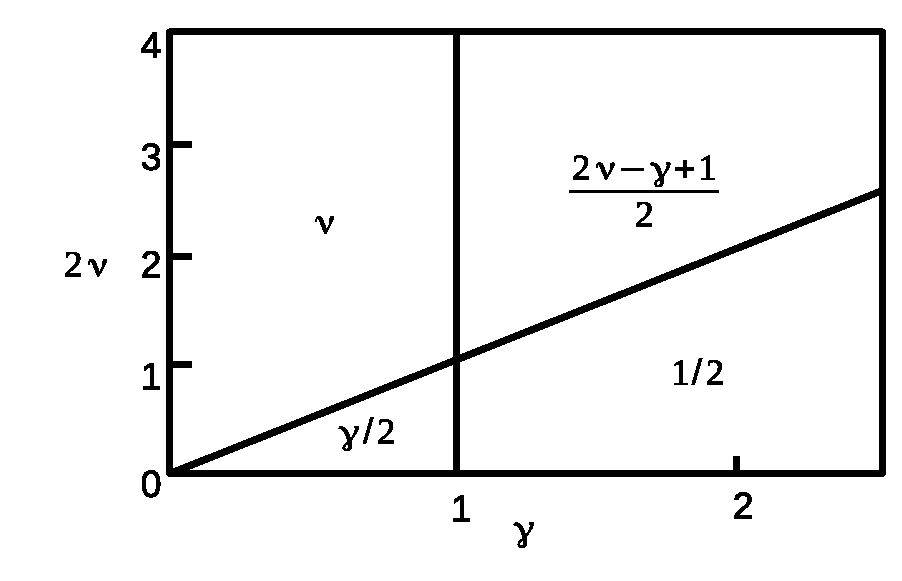
\includegraphics[width=90mm]{pics/alphaValuesPDF.eps}
\caption{Values of $\alpha$ in the different regions of parameter space. Solid lines correspond to changes in the regime.
\label{fig:alphaValuesPDF} }
\end{center}
\end{figure} 
%
There is no known solution for the inverse Laplace transform of this expression for general values of $\alpha$. However for the special case of $\alpha = \frac{1}{2} $ the result is known to be
%
\begin{align}
\gls{pdf}_{\alpha=1/2}(x|t) = \frac{1}{\sqrt{\pi}t}e^{-\frac{1}{4t}\abs{x}^2} ,
\end{align}
%
i.e. a Gaussian distribution with variance $\sqrt{2t}$. \\

For the very similar one-side alpha-stable L\'evy distribution, whose Laplace transform reads
%
\begin{align}
f(s) = e^{-s^{\alpha}},
\end{align}
%
there exists a closed expression for all rational $\alpha<1$ derived in \cite{penson2010}, where the result is expressed in generalized hypergeometric functions. This can be related to our case via the Riemann-Liouville fractional derivative of order $\alpha-1$ \cite{mathai2009}. Unfortunately I was not able to find a closed expression for this result that could be evaluated.\\
However the second factor $e^{-\abs{x}s^{\alpha}}$ is always slowly varying in the limit $s \to 0$, therefore the Tauberian theorem in Eq. (\ref{eqn:tauberian}) tells us that the leading order of the inverse Laplace transformation will be proportional to $t^{-\alpha}$. While this loses the exact dependence on $\abs{x}$ it does predict how the \gls{PDF} will scale at the origin $\abs{x}=0$, which can be compared to the results of the simulation.\\

We can furthermore evaluate the inverse transform numerically using the powerful algorithm developed by Talbot \cite{talbot1979}, which I mentioned earlier. The results of this are presented in Sec. \ref{analyticResultsPDF}. %Analytical Calculations
\chapter{Results and Discussion}

\section{Ordinary MSD}



The results for the \gls{msd} in the ordinary case found in Eq. \ref{balpoint} can are summarized in Fig. \ref{fig:resultsMSDordinary}

\begin{figure}[h!]
\begin{center}
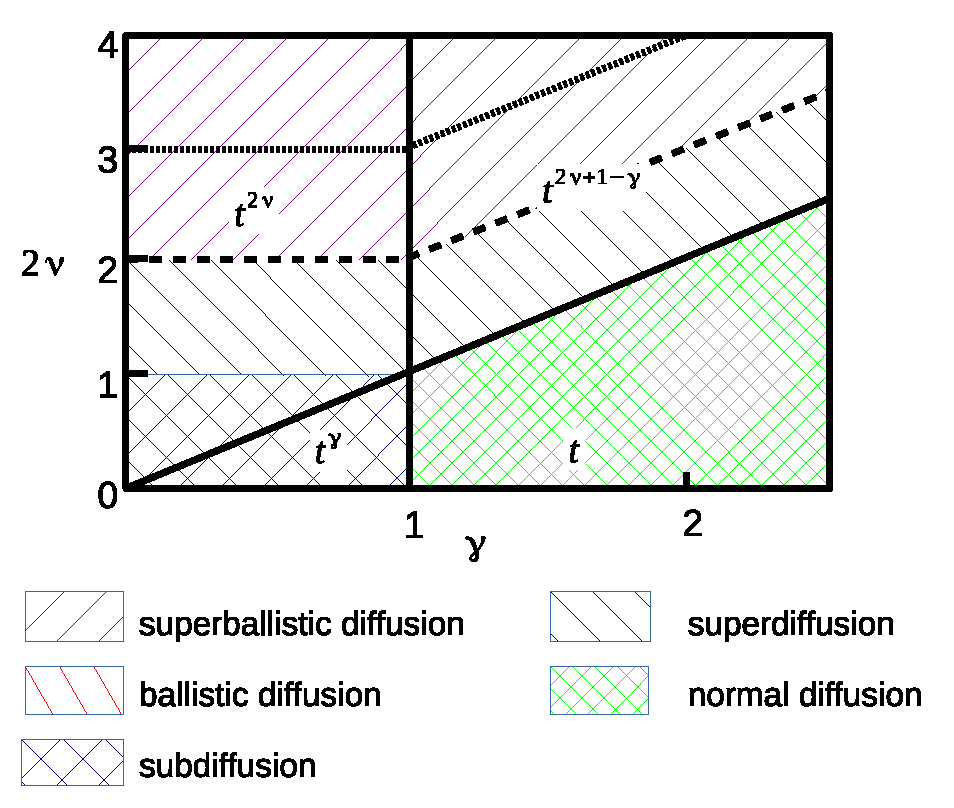
\includegraphics[width=90mm]{pics/resultsMSDordinary.eps}
\caption{The picture shows the asymptotic time dependence of the ensemble average $\langle x^2 \rangle \propto t^{x}$ in the ordinary L\'evy walk. The thick solid lines correspond to the changes in time exponent while the hatchings indicate the type of diffusion. The dashed line corresponds to ballistic behavior and the dotted one to the Richardson law.
\label{fig:resultsMSDordinary} }
\end{center}
\end{figure} 

We see that sub- as well as superdiffusion are realized in the ordinary case and that we can even reach superballistic diffusion for large values of $\eta$. This includes the Richardson regime, which is achieved for $\nu = 3/2$ for $\gamma <1$, and for $\nu = (\gamma + 2)/2$ for $\gamma > 1$. Also note that the area of normal diffusion is confined to the parameter ranges of $\gamma>1$, $2\nu < \gamma$. This corresponds to finite step duration and mean squared step length, which means the asymptotic \gls{PDF} is subject to the central limit theorem. We therefore expected normal diffusion in this region, which is confirmed by the results shown here.\\

We also see that the new parameter $\eta$ does not affect the time dependence, as it only affects the prefactor in leading order. Instead it governs the divergence that arises when calculating the second marginal moment of the distribution of incomplete steps, $r_2(t)$. Here we rederive the condition of convergence found in \cite{radons2018}, $\gamma > 2(\nu - \eta)$, which in the picture corresponds to the area below a diagonal line parallel to the bold one whose offset is given by $2\eta$. Increasing $\eta$ therefore increases the area of finite MSD in the picture, with $\nu=\eta$ always resulting in a finite MSD (since $\gamma >0$). From this we can see that for the original model with $\eta =1$ the Richardson regime for is either over or exactly on the line and therefore divergent. \\

These results where tested through simulation, with an ensemble of $10^5$ particles. To ensure that the particles had time to reach the asymptotic behavior of $t>>t_0$ the last observation time was set to $t_{max} = 20000$
\footnote{All times are multiples of $t_0$, which was set to 1 in the simulation. Similarly all lengths are multiples of $c t_0^{\nu}$, which is also set to 1. }
I have then fitted the simulation results with $f(x) = a \; x^b$, with $b$ being the time exponent from the analytical calculations. We see in Fig. \ref{fig:plotMSDordinary} that the \gls{msd} indeed follows a power law, with the time exponent being in good agreement with the analytic predictions. This was tested further with simulations run with various configurations of $\gamma$, $\nu$ and $\eta$ and the  deviation from the predicted exponent was always smaller than 0.04. These small deviation can be explained by the influence of subleading terms for finite $t_{max}$. The simulation therefore confirms the results of the analytical calculation.
%
\begin{figure}
\begin{center}
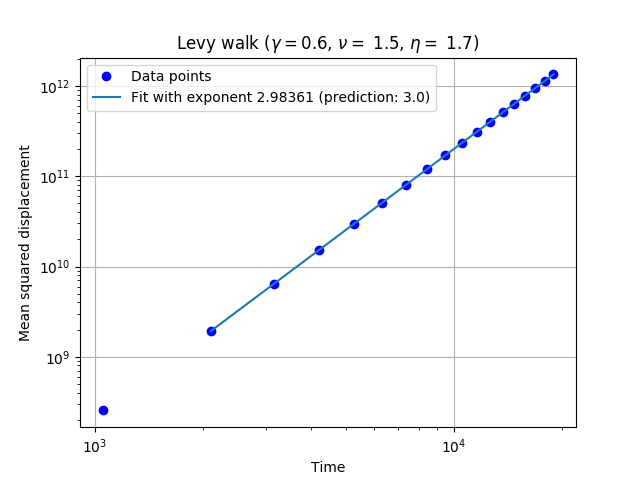
\includegraphics[width=120mm]{pics/plotMSDordinary.png}
\caption{Time dependence of the ordinary MSD. The data was fitted with $f(x) = ax^b$.
\label{fig:plotMSDordinary} }
\end{center}
\end{figure} 
%

\todo{analyze regions of behavior along the lines of where step length and step variance diverge}

\section{Aged MSD}

For short aging times we reproduce the behavior of the ordinary walk in leading order up to prefactors, which is to be expected as the ordinary and aged results should coincide in the limit of $t_a \to 0$. We also find that in addition to $\gls{rest}_2(t)$ there is now a second possibly divergent contribution from $\gls{single}_2(t)$, but both have the same condition of convergence as the ordinary case, $\gamma > 2(\nu-\eta)$. \\

For long aging times the region is the same, but the behavior of the walker differs significantly, which is illustrated in Fig. \ref{fig:resultsMSDaged}. 
%
\begin{figure}[h!]
\begin{center}
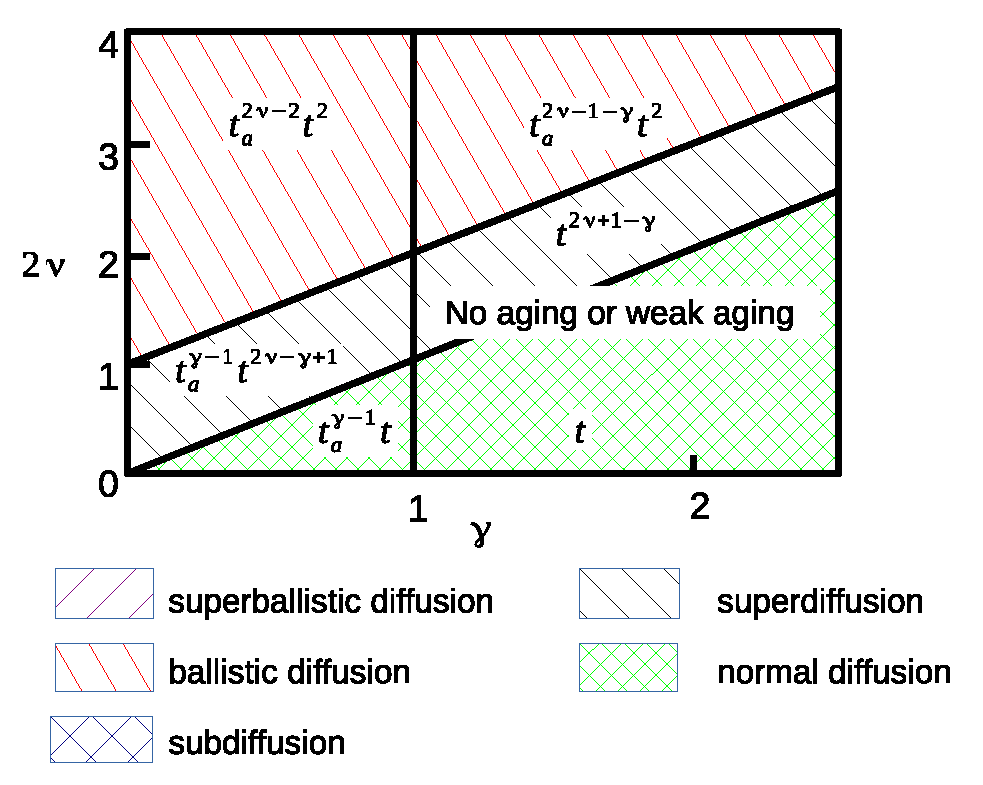
\includegraphics[width=90mm]{pics/resultsMSDaged.eps}
\caption{The panel shows the behavior of the ensemble average $\langle x^2(t) \rangle$ for the L\'evy walk in the limit of long aging times. The thick solid lines correspond to the changes in time-dependences while the hatchings represent the type of diffusion. The dashed line corresponds to the ballistic behavior, and the dotted one to the Richardson law.
\label{fig:resultsMSDaged} }
\end{center}
\end{figure} 
%
We see that for the parameter range where the ordinary walk showed subdiffusion we now find regular diffusion but with a prefactor that decays with growing aging times. There is no longer any superballistic diffusion and thus also no Richardson regime. However this does not make the model unsuitable for the description of the Richardson regime, since that relates to measuring the distance between two tracers immediately after they have been released into a stationary flow, i.e. corresponds to the ordinary case.\\ Furthermore we see that the aging leaves the parameter region with finite mean step duration ($\gamma<1$) unchanged wherever the ordinary walk showed normal or superdiffusive behavior ($2\nu < \gamma +1$).\\
The results for convergence are similar to the previous cases in that the second moment only exists for $\gamma>2(\nu-\eta)$, and if it exists the value of $\eta$ only enters the prefactors, but does not change the asymptotic power law dependences of the MSD, similar to the ordinary case.\\

It is noteworthy that the highest possible time exponent in the aged walk is quadratic, which seems counterintuitive since for small $\gamma$ long aging times correspond to an ensemble that is dominated by steps whose duration is much longer than the observation time and whose contribution to the \gls{msd} should scale strongly with time for large $\nu$. However this does not mean that the walkers move "slower" in the aged case but rather a result of the first order approximation in the observation time: Consider a walker whose step begins long before the beginning of observation at $-t_a$ and continues until the end of observation at $t$. His squared displacement during the observation is given by
%
\begin{align}
|x|^2 =& [c (t_a+t)^{\nu} - c (t_a+t)^{\nu-\eta} (t_a)^{\eta} ]^2\\
\simeq & c^2 \eta^2  (t_a+t)^{2\nu-2\eta} t_a^{2 \eta -2} t^2 \\
\simeq & c^2 \eta^2 t_a^{2 \nu -2} t^2 ,
\end{align}
%
which is exactly the result we see found for the parameter $\gamma <1$ and $2\nu > \gamma+1$ where such contributions dominate. The high speed of these cases is now shifted from the $t$ dependence to the prefactor which scales with $t_a$, similar to the way previously sudiffusive parameter ranges have now a prefactor that shrinks with larger aging times.\\

We moreover note that the double time-ensemble average $\langle \langle x^2 (t) \rangle_T \rangle_E$, also discussed in Ref. \cite{radons2018}, whose calculation involves an additional integration over the time,$\langle \langle x^2 (t) \rangle_T \rangle_E \simeq (T-t)^{-1} \int_0^{T-t} \langle x^2 (t|t_a) \rangle dt_a$  shows the same behavior as the aged walk if the measurement time $t$ is associated with the time lag in the double average, and the aging time $t_a$ is changed for the data acquisition time $T$.   \\

The verification via the simulation now involved the fitting of the MSD with regards to the observation as well as the aging time. The former was done analogously to the previous section and showed good agreement. For the aged time however considerable longer times where need, as both $t>> t_0$ and $t_a>> t$ had to be satisfied to reach the asymptotic limit. For an ensemble of $10^5$ walkers with $t_{max}=5\; 10^{3}$ and $t_{a,max} = 10^{6}$ the aging time exponent is in good agreement with  the analytical prediction as can be seen in Fig. \ref{fig:plotMSDaged}.
%
\begin{figure}
\begin{center}
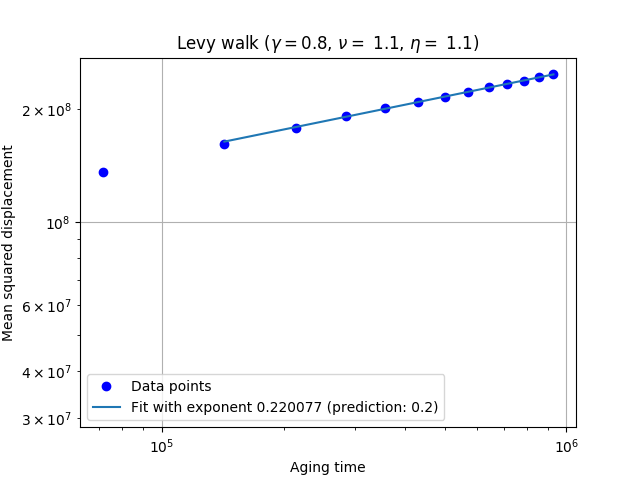
\includegraphics[width=120mm]{pics/plotMSDaged}
\caption{Aging time dependence of the aged MSD. The data was fitted with $f(x) = ax^b$.
\label{fig:plotMSDaged} }
\end{center}
\end{figure} 
%
The analytical results have again been tested for various configurations of $\gamma$, $\eta$ and $\nu$ with the highest deviation of the aging time exponent from the analytic result being 0.06, which again is caused by the computational limits of reaching the asymptotic regime.


\section{Shape of the probability density function}

The \gls{PDF} was investigated numerically in one dimension by accumulating histograms for large ensembles of $10^{9}$ walkers. Since the \gls{PDF} is symmetric only the positive side is shown in the following figures.\\

\begin{figure}[!htb] % to enforce that it doesn't become a p float, which takes up the whole page
\begin{center}
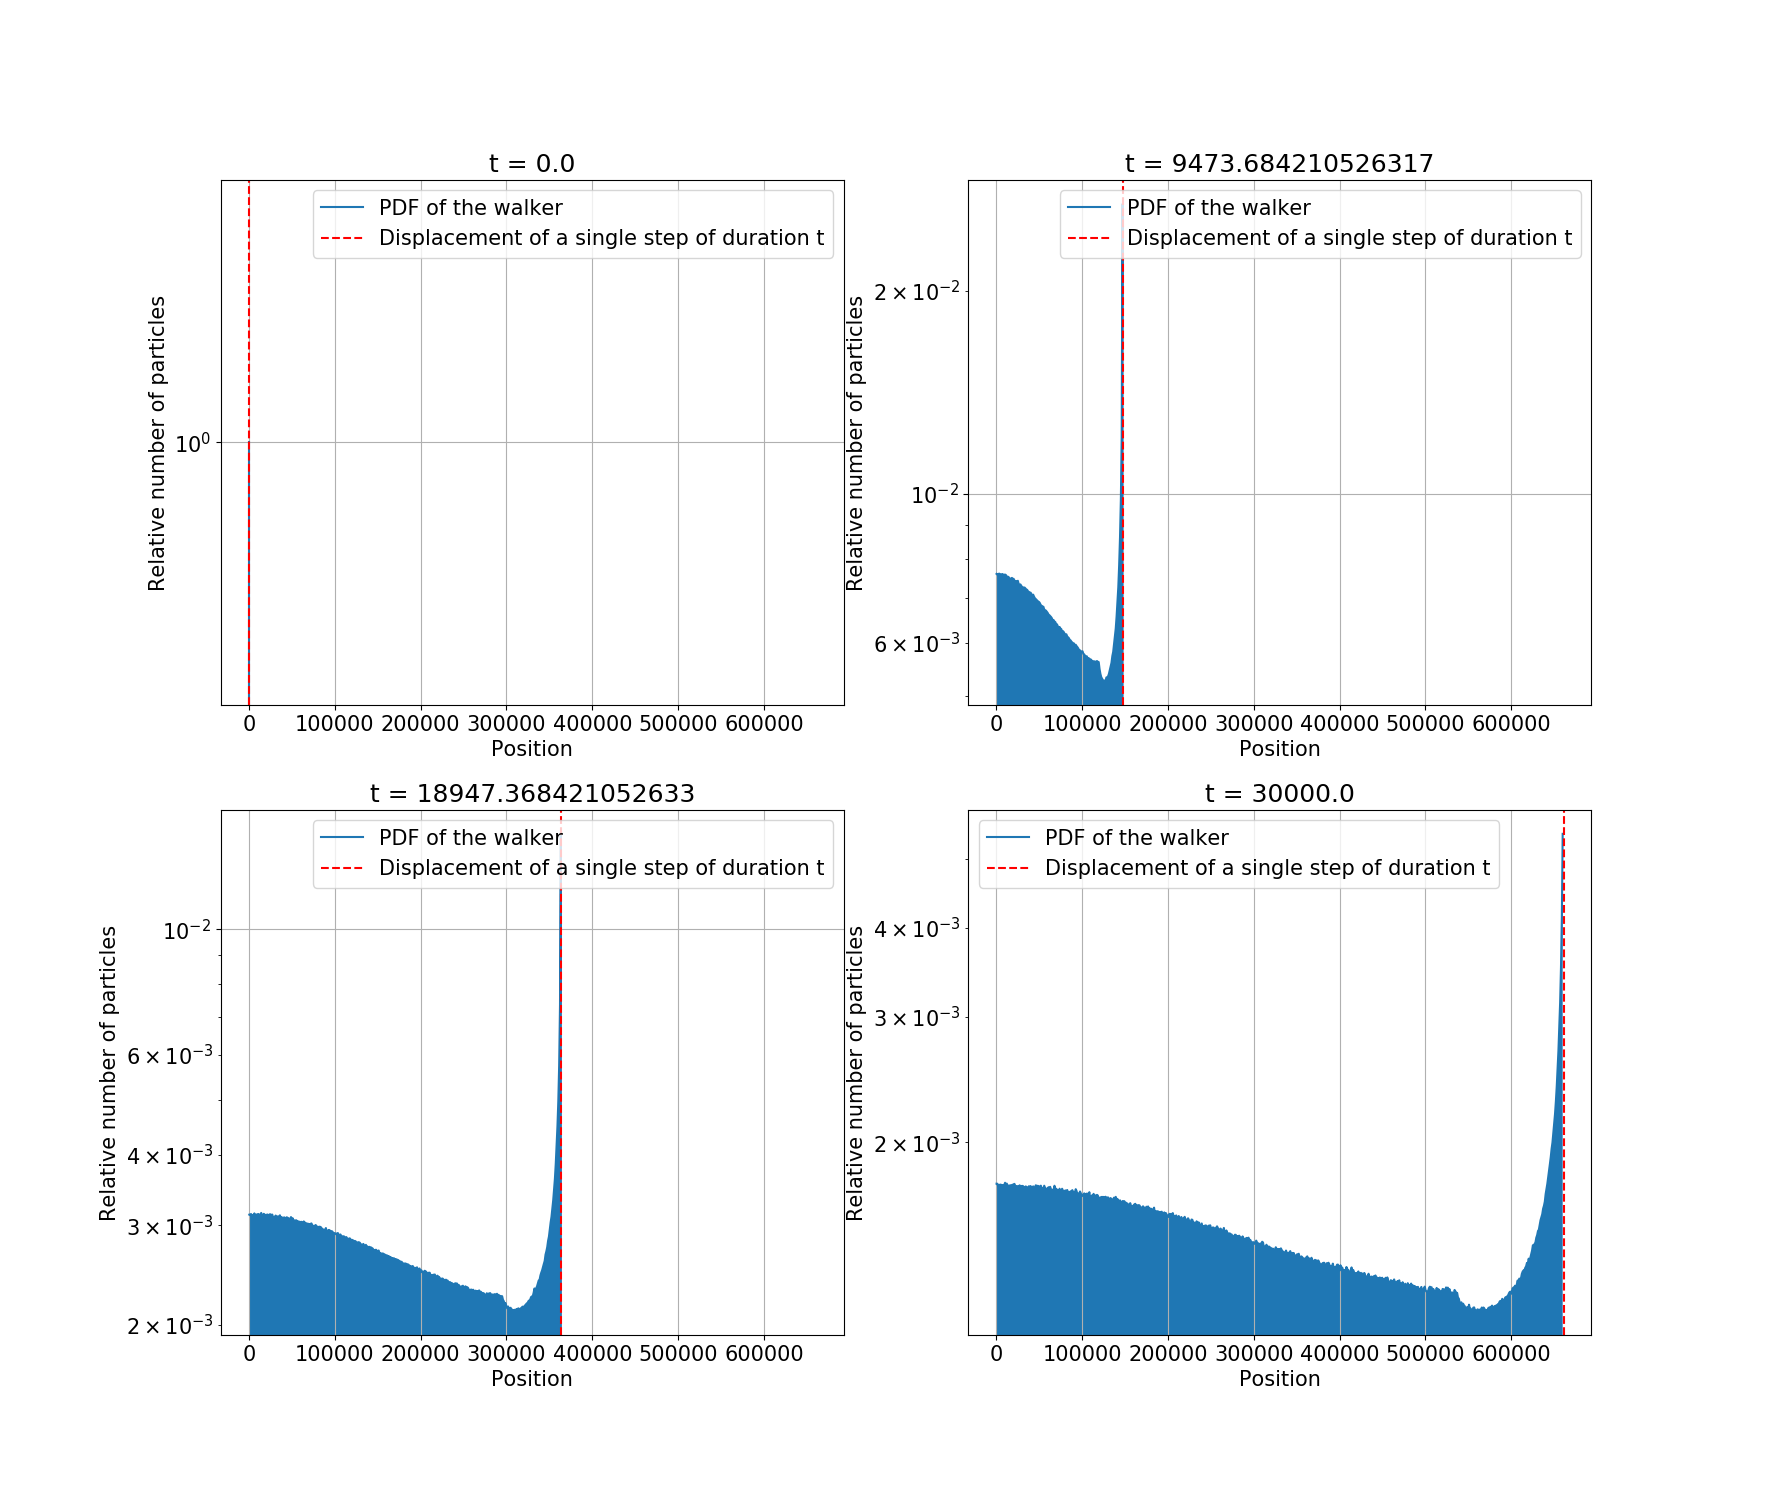
\includegraphics[width=1\textwidth]{pics/histogramShapeEtaEqual.png}
\caption{Histograms of a L\'evy walk with $\gamma =0.6$, $\nu = 1.3$ and $\eta =1.3$ at different points in time. The dashed line indicates the position a walker would have reached in a single step beginning at $t=0$ and ending exactly at the time of the respective panel.
\label{fig:histogramShapeEtaEqual} }
\end{center}
\end{figure} 
%
Unlike the \gls{msd}, where the new parameter $\eta$ only changes the prefactors of finite results,  $\eta$ has a major impact on the shape of the \gls{PDF}: \\
In the case $\nu=\eta$ shown in Fig. \ref{fig:histogramShapeEtaEqual} the histogram has a clear cutoff marked by a delta-shaped peak that coincides with the position a walker can reach in a single step of duration $t$. This is similar to what you find for the similar velocity model ($\eta=\nu=1$), \todo{source} where the \gls{PDF} also has a clear boundary after which no walker can be found. \\
This can be understood by considering the displacement in the first step of a walk,
%
\begin{align}
\abs{\ve{x}_{n+1}} = c \gls{dur}_{1}^{\nu-\eta} t^{\eta} , \label{eqn:step}
\end{align}
% 
where we recall that $\gls{dur}_{1}$ is the total duration of the step, which may be longer than the observation time $t$. In the case of $\eta=\nu$ the dependence on the total step duration vanishes, which means that any particle starting at $t=0$ moves with the same speed, regardless of how long the step will last. Since $\eta>1$ the the greatest displacement is archived when the particle performs a single step whose duration is greater or equal than the observation times. This means two things: Firstly, no particle can be found beyond this limit and secondly, the entire probability of having a step duration of $t$ or longer is concentrated on this particular cutoff, which corresponds to a delta peak in the probability density, which explains that feature of the histograms. \\
For the rest of the \gls{PDF} we see the highest probability besides the peak at the origin, which is consistent with it being a isotropic model, and then the density decays exponentially with the distance from the origin, $\gls{pdf} \propto e^{-|x|}$. Directly before the peak a minor notch can be seen in the histogram, whose origin is unclear.  \\
%
\begin{figure}[!htb] % to enforce that it doesn't become a p float, which takes up the whole page
\begin{center}
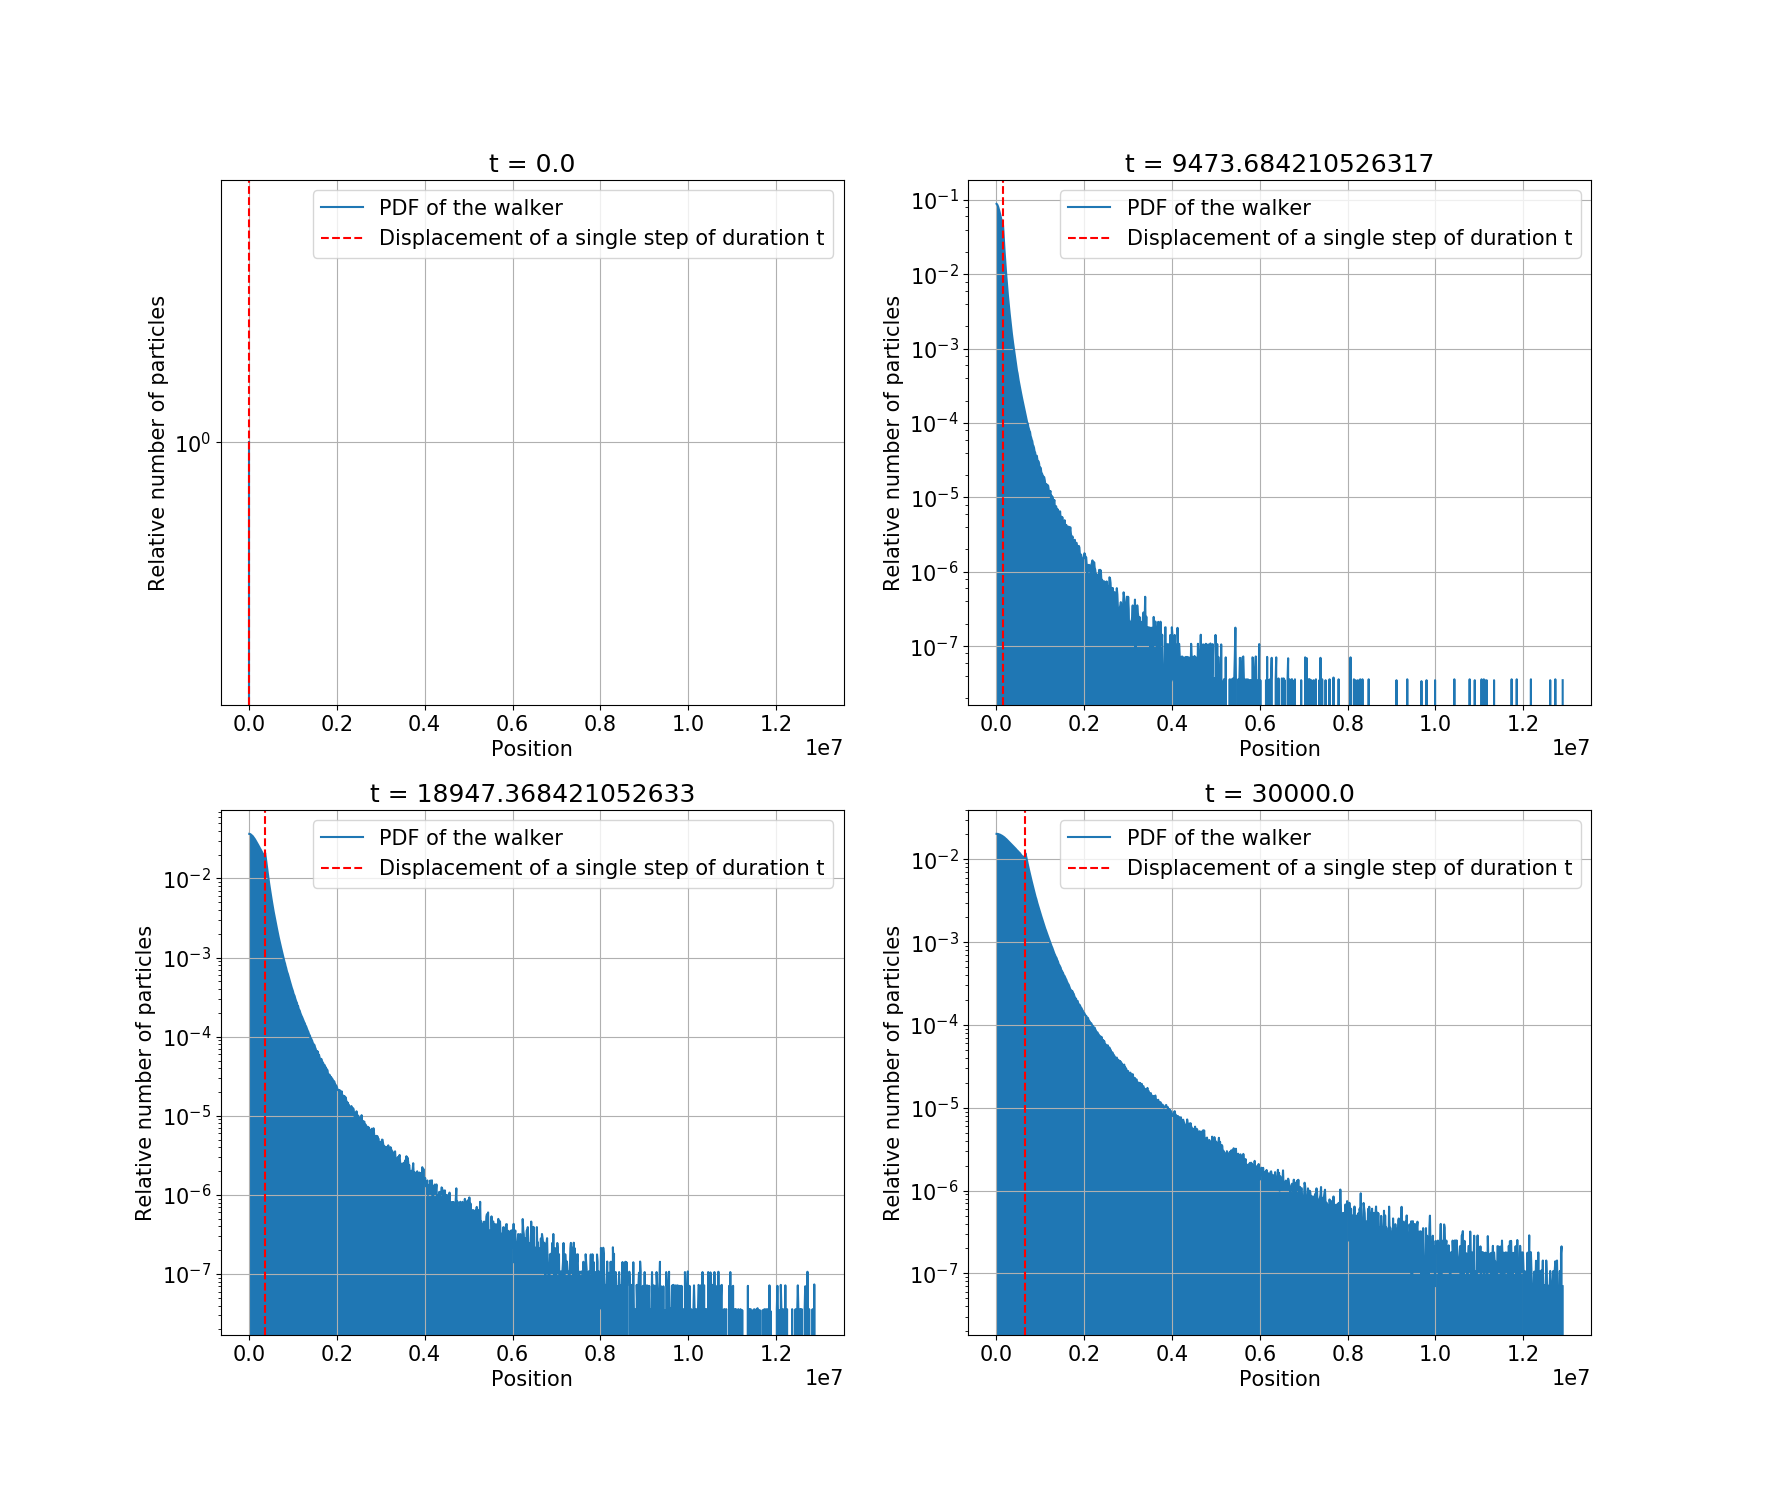
\includegraphics[width=1\textwidth]{pics/histogramShapeEtaSmall.png}
\caption{Histograms of a L\'evy walk with $\gamma =0.6$, $\nu = 1.3$ and $\eta =1.1$ at different points in time. The dashed line indicates the position a walker would have reached in a single step beginning at $t=0$ and ending exactly at the time of the respective panel.
\label{fig:histogramShapeEtaSmall} }
\end{center}
\end{figure} 

However this shape of the \gls{PDF} changes profoundly when modifying $\eta$, as can be seen in Fig \ref{fig:histogramShapeEtaSmall}: Here both $\gamma$  and $\nu$ are identical to the previous picture but $\eta$ is now smaller than $\nu$. Now walkers travel well beyond the limit of what can be reached in a single step of total duration $t$ and there is no longer a  delta peak. Instead the dashed line marks the distinction between a simple exponential decay close to the origin and a faster decay further away. \\
This shape can again be understood when considering Eq. (\ref{eqn:step}): Since $\eta < \nu$ the observation time independent prefactor of the displacement now grows with the total step duration. This means that walkers whose step duration is larger than the observation time can reach arbitrarily high initial velocities and therefore move well beyond the dashed line. Consequently the walker has a finite probability to be at any point for $t>0$, which is not fully captured here since the histogram only covers a finite range and the positions of walkers that move beyond the histogram range cannot be shown. \\
Also note that while very long steps are not extremely rare (the mean step duration diverges in the case $\gamma >1$) for finite ensembles these outliers are nevertheless hard to capture and even for $10^{9}$ walkers we see the limits of the simulation in the edges of the \gls{PDF}, where it becomes discontinuous. 
%
\begin{figure}[!htb] % to enforce that it doesn't become a p float, which takes up the whole page
\begin{center}
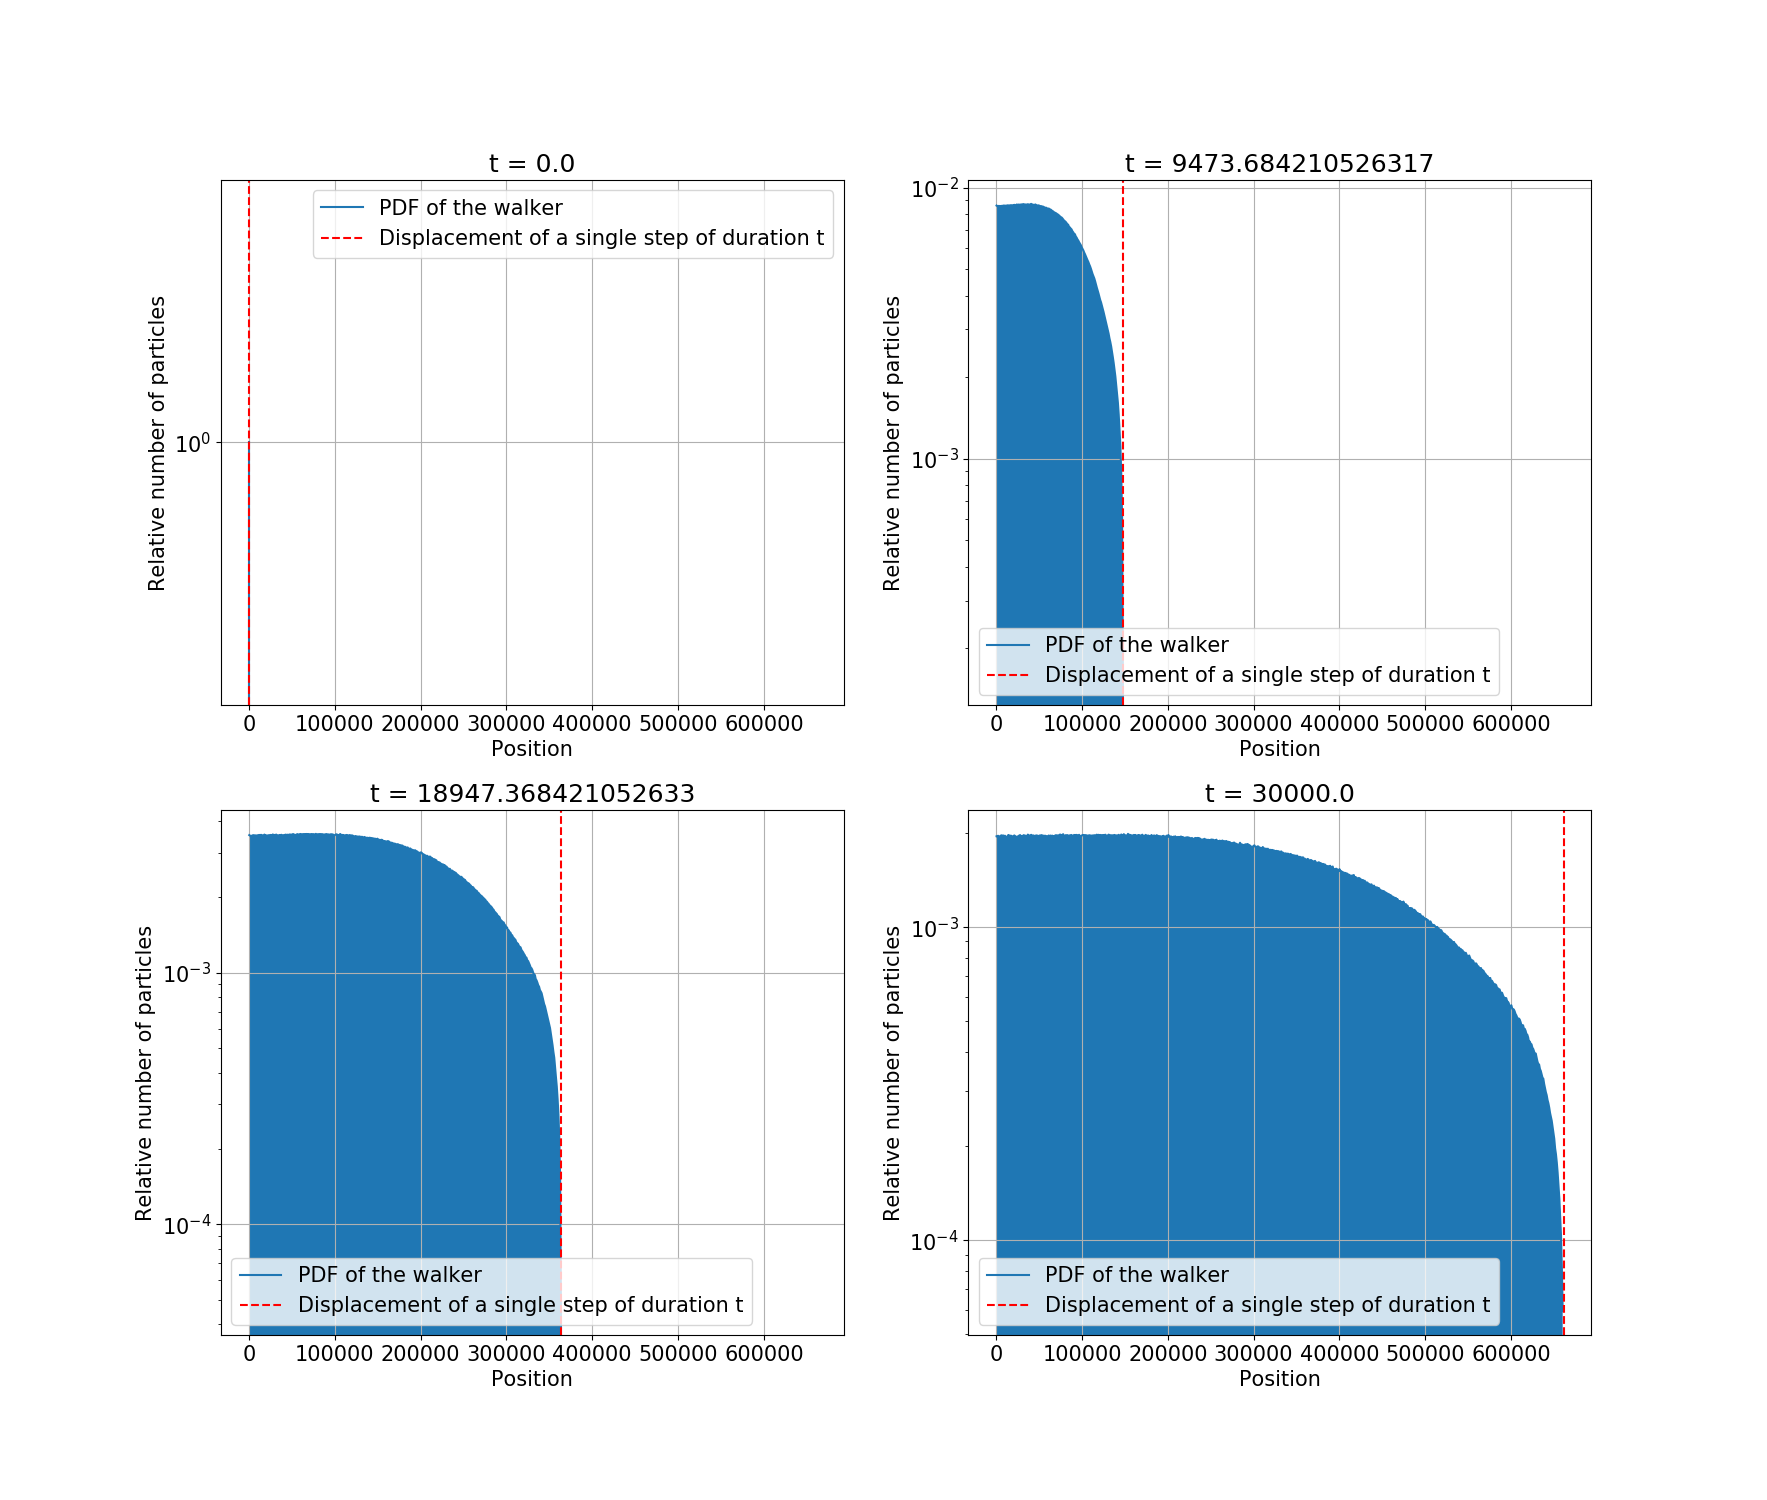
\includegraphics[width=1\textwidth]{pics/histogramShapeEtaLarge.png}
\caption{Histograms of a L\'evy walk with $\gamma =0.6$, $\nu = 1.3$ and $\eta =1.5$ at different points in time. The dashed line indicates the position a walker would have reached in a single step beginning at $t=0$ and ending exactly at the time of the respective panel.
\label{fig:histogramShapeEtaLarge} }
\end{center}
\end{figure} 

Moving on to the case of $\eta> \nu$ as shown in Fig. \ref{fig:histogramShapeEtaLarge} we see that the shape of the \gls{PDF} is again very different: Similar to the $\eta = \nu$ case the dashed line marks a clear limit of how far a walker can reach, but there is no delta peak. Inspecting Eq. (\ref{eqn:step}) again we see the reason: Because we have $\eta> \nu$ the prefactor in the displacement actually grows smaller with increasing total step duration, meaning that any walker performing a step with duration longer than $t$ can actually not reach the limit, meaning that only walkers with a step duration of exactly $t$ can reach the cutoff, the probability of which is infinitesimal. \\

These findings explain the convergence condition we rederived for the \gls{msd}, $\gamma > 2(\nu-\eta)$: For $\eta \geq \nu$ the support of the \gls{PDF} is bounded and therefore the \gls{msd} always converges. For $\eta < \nu$ this is no longer the case and there is a finite probability to find the walker at any distance from the origin for $t>0$. Convergence now depends on the likelihood of extreme events, meaning that $\gamma$ has to be sufficiently large for the \gls{msd} to exist.\\
%
\begin{figure}[!htb] % to enforce that it doesn't become a p float, which takes up the whole page
\begin{center}
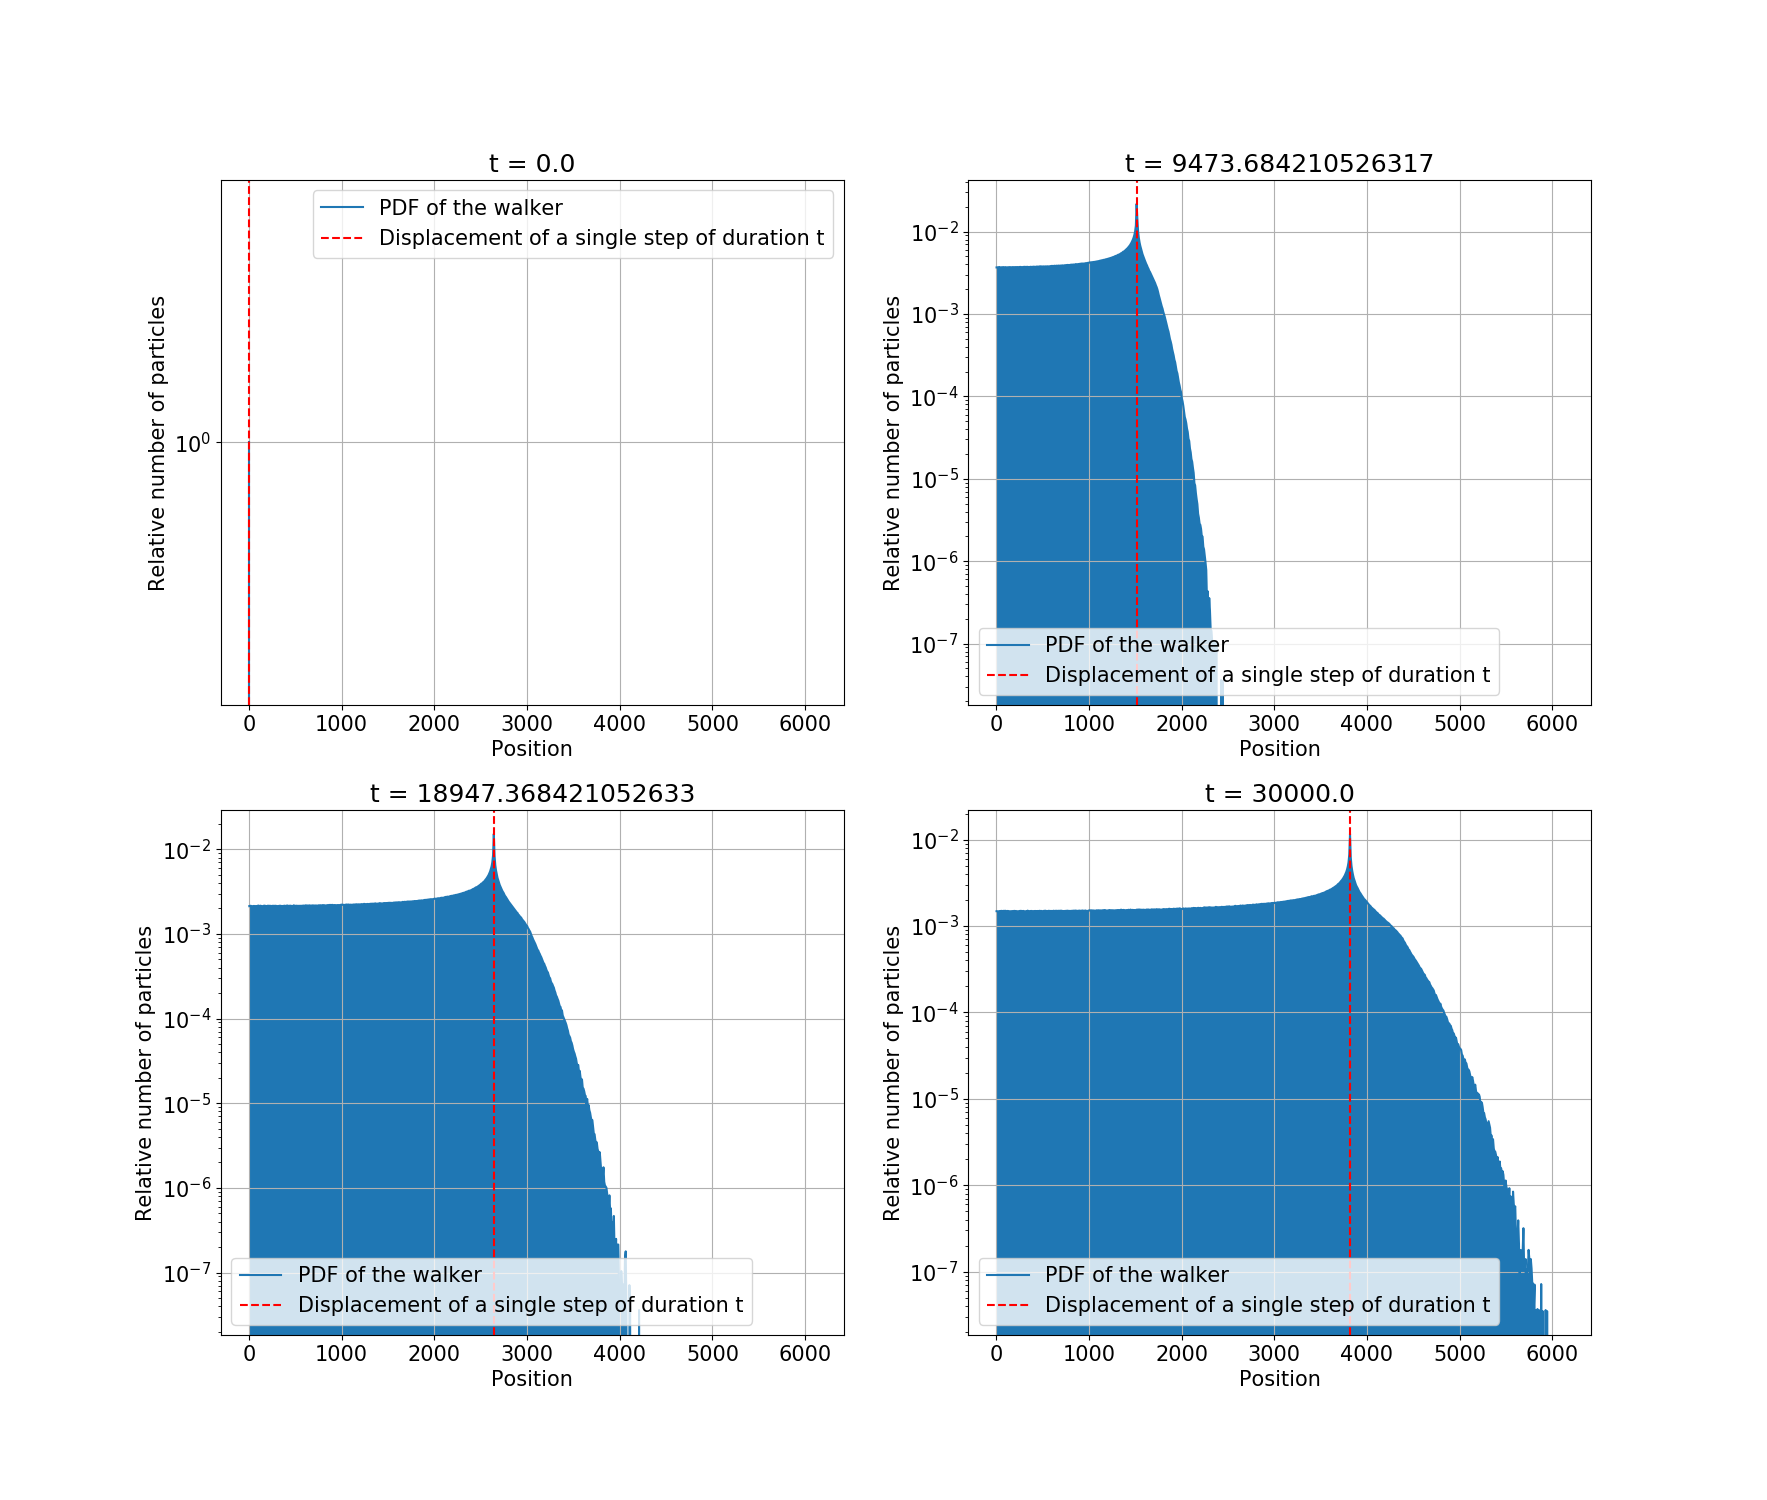
\includegraphics[width=1\textwidth]{pics/histogramShapeNuSmall.png}
\caption{Histograms of a L\'evy walk with $\gamma =0.6$, $\nu = 0.8$ and $\eta =0.8$ at different points in time. The dashed line indicates the position a walker would have reached in a single step beginning at $t=0$ and ending exactly at the time of the respective panel.
\label{fig:histogramShapeNuSmall} }
\end{center}
\end{figure} 

Next we are interested in the influence of the parameter $\nu$ on the shape of the \gls{PDF}, which is illustrated in Fig. \ref{fig:histogramShapeNuSmall}: We are again in the case of $\eta = \nu$, but unlike in Fig. \ref{fig:histogramShapeEtaEqual} the dashed line no longer marks a sharp boundary of the \gls{PDF} and there is a finite probability for a walker to be found beyond it. However this is not due to steps with durations longer than the observation time (all these cases reach exactly the boundary and contribute to the peak) but instead due to walkers that take more than one step: Since $\nu<1$ the maximum displacement is not realized by making a single long step, but rather by taking many smaller steps in the same direction, simply because the sum of a root is larger than the root of a sum. It follows that values of $\nu<1$ cause the breakdown of the sharp cutoff and the simulations show that this effect becomes more impactfull with smaller $\eta$. {\color{red} However this does not cause divergence of the \gls{msd} because so many steps are almost never realized for power law step duration distributions.  }\\

\begin{figure}[!htb] % to enforce that it doesn't become a p float, which takes up the whole page
\begin{center}
\includegraphics[width=1\textwidth]{../CUDA_Simulation_RW/Results/Histograms/{histogram_gamma_1.2_nu_1.3_eta_1.3_ta_0}.png}
\caption{Histograms of a L\'evy walk with $\gamma =1.2$, $\nu = 1.3$ and $\eta =1.3$ at different points in time. The dashed line indicates the position a walker would have reached in a single step beginning at $t=0$ and ending exactly at the time of the respective panel.
\label{fig:histogramShapeGammaLarge} }
\end{center}
\end{figure} 
%
Finally we consider the effect of varying $\gamma$ on the \gls{PDF} which is shown in in Fig. \ref{fig:histogramShapeGammaLarge}. Comparing this to Fig. \ref{fig:histogramShapeEtaEqual}, which differs only in its $\gamma$ value, we see that the peak is much less prominent but the position of the cutoff doesn't change. Furthermore we see that the \gls{PDF} is much more centered on the origin . This makes sense as a larger value of $\gamma$ makes steps longer than the observation time much more unlikely and the walk is therefore less dominated by these extreme events, which were contributing to the height of the delta peak.

\section{Probability density at the origin}

From the analytical approximation of the \gls{PDF} follows a prediction for the time dependence of  the probability density at the origin, which was tested in the simulation. The results of the analytical calculation are shown in Fig. \ref{fig:resultsPDF}.
%
\begin{figure}[!htb] % to enforce that it doesn't become a p float, which takes up the whole page
\begin{center}
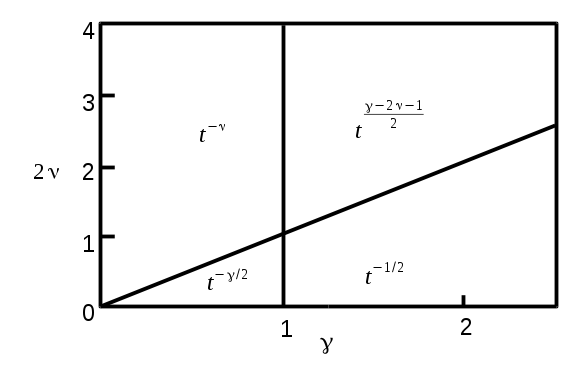
\includegraphics[width=0.8\textwidth]{pics/resultsPDF.png}
\caption{The time dependence of the probability density for different values of the parameters $\nu $ and $\gamma$ is shown. Thick lines indicate the distinction between two different regimes.
\label{fig:resultsPDF} }
\end{center}
\end{figure} 
%
By plotting the change in the \gls{PDF} at the origin over a period double logarithmically we can extract the time exponent, as is shown in Fig. \ref{fig:fitPDFOrigin}.
%
\begin{figure}[!htb] % to enforce that it doesn't become a p float, which takes up the whole page
\begin{center}
\includegraphics[width=0.8\textwidth]{../CUDA_Simulation_RW/Results/Histogram_origin_peak/{origin_peak_gamma_1.5_nu_0.8_eta_0.8}.png}
\caption{A fit of time dependence of the probability density for the parameter values $\gamma=1.5$, $\nu =0.8 $ and $\eta=0.8$ is shown in a doubly logarithmic plot.
\label{fig:fitPDFOrigin} }
\end{center}
\end{figure} 
%
We see that the \gls{PDF} is indeed of the form $t^{x}$ and the deviation of the time exponent from the expected result, $t^{-0.55}$, are small. Fits with various other parameters confirm this result, with deviations always being smaller than 0.02
 %Results and Discussion
\chapter{Conclusions}

% question was how eta in generalized model changes things
The main question in this thesis is how the introduction of a new acceleration parameter $\eta$ into the widely used L\'evy walk model changes its properties, and in particular what its effect on the recently found divergence in the \gls*{msd} of the L\'evy walk are. \\
To this end the asymptotic behavior of the \gls*{msd} was calculated in one dimension, both for the ordinary and for the aged walk, which can be found in 
\cite{bothe}. 
We showed that \gls*{msd} is finite when the condition $\gamma > 2(\nu-\eta)$ is satisfied, not just in the ordinary case, where this was already known\cite{radons2018}, 
but for the aged case as well. This means that the introduction of $\eta$ is indeed suitable to avoid the divergence of the original model. \\
Furthermore we found that $\eta$ does not affect the asymptotic time dependence of the \gls*{msd}, meaning that for the ordinary walk, all diffusion regimes can be recovered from the original model for suitable values of $\eta$, including the superballistic Richardson regime. \\
Additionally it was shown that in the limit of long aging times neither subdiffusion nor superballistic diffusion can be found in the generalized model, which was previously unknown.

A similar calculation attempted to find the asymptotic behavior of the \gls*{PDF}, but this could unfortunately not be done analytically for general parameter values. It was however possible to extract the correct time dependence of the probability density at the origin and to derive a correct analytical solution in the domain of applicability of the central limit theorem. For the other cases a numerical evaluation of the expression resulted in a \gls*{PDF} that was not able to capture the rich behavior revealed in a simulation of the process. 

For this simulation CUDA parallel computing was utilized to validate the findings for the \gls*{msd} and to create histograms for both the aged and the ordinary case. Here we show significant differences in the \gls*{PDF} for different values of the parameters $\gamma$ and $\nu$. Interestingly the new parameter $\eta$ also has a major influence on the \gls*{PDF}, as it governs the formation of delta peaks as well as the existence of a cutoff for the \gls*{PDF}, which explains $\eta$'s role in the convergence condition above. The results can mostly be explained heuristically by analyzing the influence of long steps on the process. \\
We also find significant aging effects for the \gls*{PDF}, which can be explained by a similar analysis.

A goal for future work would be to find an analytical expression that can describe the features of the PDF quantitatively. One approach could be the incorporation of higher order terms into the asymptotic expansion in this work, which can be done straightforwardly. It is however not immediately clear if this would capture the effect of $\eta$ on the \gls*{PDF}, so another approach might be more suitable.\\
It should also be noted that this thesis focuses very much on the theoretical aspects of the model, so it would be interesting how the different values of $\eta$ could be realized in experimental settings. A natural candidate would be the case $\eta=\nu=2$, corresponding to a process with constant acceleration, which has been investigated in 
\cite{burioni2013rare, burioni2014scaling}.

To summarize, we show that the generalized L\'evy walk does indeed allow for the recovery of the diffusion regimes that were divergent in the original model. Furthermore we find that he introduction of $\eta$ has a significant impact on the \gls*{PDF}, which should be investigated further.

 %Conclusions
% usw.

%-Anhang----------------------------------------------------------

\appendix
\chapter{The Tauberian theorem} \label{sec:tauberian}

In this thesis I often consider Laplace transforms of functions asymptotically following power laws. The asymptotic form of Laplace transforms of functions which at long times behave as $f(t) = t^{\rho-1} L(t)$, where $L(t)$ is a slowly varying function, in the asymptotic regime $s \to 0$ as well as the corresponding inverse transforms may be obtained by use of the Tauberian theorem. \\

We assume that a Laplace transform $f(s) = \int_0^t f(t) e^{-st} dt$ exists, i.e. the function $f(t)$ does not possess a strong divergence at 0. All functions $f(t)$ appearing this thesis are non-negative. For such functions Laplace transforms are monotonically decaying functions of $s$. Depending on the behavior of $f(t)$ at infinity two cases should be considered: \\
The function $f(t)$ might be integrable on $[0, \infty)$, so that 
$\int_0^\infty f(t) dt = I_0^{f} < \infty$, or this integral may diverge. The first case corresponds to $\rho < 0$ and 
the second one to $\rho > 0$ (the case $\rho = 0$ may belong to the either class depending on the concrete form of $L(t)$). \\
In the second case the Tauberian theorem may be applied immediately, stating that if $f(t)$ is a regularly varying function, i.e. when  its Laplace transform is given by 
\begin{equation}
 f(t) \simeq t^{\rho-1} L(t) \;\; \leftrightarrow \;\; f(s) \simeq \Gamma(\rho) s^{-\rho} L\left(\frac{1}{s}\right)
 \label{eq:Tauberian}
\end{equation}
for $\rho \geq 0$. As in the main text, all slowly varying functions will be omitted (i.e. changed for constants $L$). 

We note that for $\rho < 0$  equation, i.e. when $f(t)$ is integrable, equation (\ref{eq:Tauberian}) suggests $f(s)$ being a growing function of $s$ and is therefore wrong. In this case let us consider the function
\begin{equation}
 S(t) = \int_t^\infty f(t') dt'.
\end{equation}
The integrability of $f(t)$ means that $S(t)$ is well-defined, and that $I_0^{f} =  \int_0^\infty f(t') dt' = S(0)$ is finite. 
The function $S(t)$ has the power-law asymptotics
%
\begin{equation}
 S(t) \simeq - \frac{L t^\rho}{\rho},
\end{equation}
and, if this is no more integrable (i.e. for $\rho > -1$), can be transformed via the Tauberian theorem, so that
\begin{equation}
 S(s) \simeq - L \frac{\Gamma(\rho+1)}{\rho} s^{-(\rho +1)} = - L \Gamma(\rho)  s^{-(\rho +1)},
\end{equation}
%
where in the last equality the identity $\Gamma(x+1) = x \Gamma(x)$ was used. 
Noting that $f(t) = - \frac{d}{dt}S(t)$ and using the Laplace representation of the derivative, we get 
\begin{equation}
 f(s) = S(t=0) - s S(s) = I^{f}_0 - L \Gamma(\rho)  s^{-\rho} .
\end{equation}
The direct application of the Tauberian theorem would give us a correct form of the second term (up to a sign), but omit the first one. 

If $S(t)$ is still integrable, we consider the function $P(t) = \int_t^\infty S(t') dt'$, whose power-law asymptotics for $t \to \infty$ is
\begin{equation}
 P(t) \simeq \frac{L t^{\rho+1}}{\rho (\rho+1)},
\end{equation}
and whose connection to $f(t)$ is given by $f(t) = \frac{d^2}{dt^2}S(t)$. For $-2 < \rho$ the function $P(t)$ is not integrable, 
and the application of the Tauberian theorem gives
\begin{equation}
 P(s) = L \frac{\Gamma(\rho+2)}{\rho (\rho+1)} s^{-\rho-2} = L \Gamma(\rho) s^{-\rho-2}.
\end{equation}
Using the Laplace representation for the second derivative we get
\begin{equation}
 f(s) = - s P(t=0) - P'(t=0) + s^2 P(s). 
\end{equation}
The value of $P'(t=0)$ is $-S(t=0)=-I^{f}_0$. The value $P(t=0)$ is given by the integral
\begin{equation}
P(t=0) = \int_0^\infty dt \int_t^\infty f(t')dt'.
\end{equation}
Changing the sequence of integrations in $t$ and $t'$ we get 
\begin{equation}
 P(t=0) = \int_0^\infty dt' f(t') \int_0^{t'} dt = \int_0^\infty t' f(t') dt'.
\end{equation}
Since $f(t)$ decays with $t$ faster than $t^{-2}$, the integral converges, and will be denoted by $I^{f}_1$. Therefore we have
%
\begin{equation}
 f(s) = I^{f}_0 - s I^{f}_1 + L \Gamma(\rho) s^{-\rho}.
\end{equation}

For $\rho < -2$ the procedure has to be repeated again for the function being the integral of $P(t)$, etc. The general result is
%
\begin{align}
 f(s) = \sum_{k=0}^{k_{\max}} \frac{(-1)^k}{k!} I^{f}_k s^k + L \Gamma(\rho) s^{-\rho}
\end{align}
%
with $k_{\max}$ being the whole part of $-\rho$, and $I^{f}_k$ being the moment integral
\begin{align}
I^{f}_k = \int_0^\infty t^k f(t) dt.
\end{align}
In the main text we never have to use more than first three terms of this expansion. 


\chapter{Estimates for the integral $I_{a,b,c}(y)$ \label{sec:integral}} 

We are interested in the integral 
%
\begin{eqnarray}
I_{a,b,c}(y) &=& \int^{1}_0 (1-z)^{b} [(z+y)^c-z^c]^2 (z+y)^{a}  dz \label{eqn:Iabc1} \\ 
&=& \int^{1}_0 (1-z)^{b} \left[ (z+y)^{a+2c} -2 (z+y)^{a+c} z^{c}  + (z+y)^{a} z^{2c}\right] dz \nonumber 
\end{eqnarray}
%
in the limit of small $y= \frac{t}{t_a} \ll 1$ for the parameter ranges $c > 0$, $b > -1$, $a \in \mathbb{R}$.

To evaluate it we use Euler's integral representation for the Gau{\ss} hypergeometric function for $\Re \; c' > \Re \; b' > 0$
\begin{eqnarray}
_{2}F_{1}(a',b';c';x) &=& \frac{1}{\mathrm{B}(b',c'-b')}    \int_{0}^{1} z^{b'-1} (1-z)^{c'-b'-1} (1-zx)^{-a'} \label{IntegralRep}. 
\end{eqnarray}
As the existence condition $1+b>0$ is always satisfied for all three terms in (\ref{eqn:Iabc1}) we can write the integral as
\begin{eqnarray}
&& I_{a,b,c}(y) = \label{eqn:Iabc2}  y^a  \left[  y^{2c} \mathrm{B}(1,1+b) _2F_1 \left(-a-2c,1;2+b; -\frac{1}{y} \right) \right.  \\
&& -2 y^{c} \mathrm{B}(1+c, 1+b) _2F_1 \left(-a-c,1+c;2+b+c; -\frac{1}{y} \right) \nonumber \\ 
&& \left. + \mathrm{B}(1+2c , 1+b) _2F_1 \left(-a,1+2c;2+b+2c; -\frac{1}{y} \right) \right]  \nonumber 
\end{eqnarray}
with $\mathrm{B}(x,y)$ being the Beta function. 
Athough the integral can be expressed in terms of three Gau{\ss} hypergeometric functions,
its investigation is somewhat tricky, since the asymptotic regimes appear as a subleading terms 
in a sum of three large contributions whose leading terms cancel. First, to avoid evaluating hypergeometric functions at $-\infty$ 
we make use of the Pfaff transformations:
\begin{align}
_2F_1(a',b';c';z) = (1-z)^{-b'} \; _2F_1 \left( b',c'-a';c;\frac{z}{z-1} \right) \label{Pfaff1} \\
_2F_1(a',b';c';z) = (1-z)^{-a'} \; _2F_1 \left( a',c'-b';c;\frac{z}{z-1} \right). \label{Pfaff2}
\end{align}
These two forms will be applicable in different domains of parameters. Under the transformations the argument of the corresponding functions on the r.h.s., equal to $\frac{1}{1+y}$, will tend to 1. Applying the Pfaff transformation Eq.(\ref{Pfaff1}) to the integrals in Eq.(\ref{eqn:Iabc2}) we find:
%
\begin{align*}
 I_{a,b,c}(y) = y^{1+a+2c} & \bigg[  (1+y)^{-1} \mathrm{B}(1,1+b)  \;  _2F_1 \left(1,2+a+b+2c;2+b; \frac{1}{1+y} \right)  \\ 
&  -2 (1+y)^{-1-c} \mathrm{B}(1+c, 1+b)   _2F_1 \left(1+c,2+a+b+2c;2+b+c; \frac{1}{1+y} \right) \\ 
&  + (1+y)^{-1-2c} \mathrm{B}(1+2c , 1+b)  \;  _2F_1 \left(1+2c,2+a+b+2c;2+b+2c;\frac{1}{1+y} \right) \bigg].
\end{align*} 
%
We now use the Euler integral representation (\ref{IntegralRep}) again, but exchange the roles of $a'$ and $b'$:
%
\begin{eqnarray*}
_{2}F_{1}(a',b';c';x) &= &\frac{1}{\mathrm{B}(a',c'-a')}  \int_{0}^{1} z^{a'-1} (1-z)^{c'-a'-1} (1-zx)^{-b'} 
\end{eqnarray*}
%
for $\Re \; c' > \Re \;  a' > 0$. Note that the existence condition for the integrals is the same as before, $b+1>0$, which is satisfied for all cases relevant in this thesis, so we can write:
%
\begin{eqnarray*}
I_{a,b,c}(y) = y^{1+a+2c} &&   \int_{0}^{1}  \left[  (1+y)^{-1}  (1-z)^{b} \left( 1- \frac{z}{1+y} \right)^{-2-a-b-2c}  \right. \\ 
&& \qquad \left. -2 (1+y)^{-1-c} z^c (1-z)^{b} \left( 1- \frac{z}{1+y} \right)^{-2-a-b-2c} \right. \\ 
&& \qquad \left. + (1+y)^{-1-2c} z^{2c} (1-z)^{b} \left( 1- \frac{z}{1+y} \right)^{-2-a-b-2c} \right] dz .
\end{eqnarray*}
The integrals of each of three contributions in square brackets would diverge for $y \to 0$, but the integral of whole sum is convergent for $a+2c < 1$ since for $y \to 0$ the integrand tends to 
\[
(1-2 z^{c} + z^{2c}) (1-z)^{-2-a-2c} =  (1-z^c)^2 (1-z)^{-2-a-2c},
\]
and the integral
\[
 C(a,c) = \int_0^1 (1-z^c)^2 (1-z)^{-2-a-2c} dz
\]
of this expression converges in the range $a+2c <1$ (to prove the convergence it is enough to expand the first term in vicinity of $z=1$). 
This integral cannot be expressed in terms of ``simple'' functions, but the (loose) bounds for it follow easily. 

Let us find two constants $B > A > 0$ such that for all $0< z < 1$
\[
 A (1-z) < 1-z^c < B (1-z). 
\]
To do so consider the function
\[
 f(z)=\frac{1-z^c}{1-z},
\]
with $f(0)=1$ and with its limiting value at $z \to 1$ given by the l'H\^opital's rule $\lim_{z \to 1} = c$. 
Therefore the limit of the function at 1 is larger than its value at $0$ when $c>1$ and smaller than this value when $c<1$. For $c=1$ this function equals to unity identically.

Now we consider $c \neq 1$ and proseed to show that the 
function $f(z)$ is monotonically growing for $c>1$ and monotonically decaying for $c<1$. To show this it is enough to show that its derivative 
on $[0,1]$ does not vanish. The derivative of the corresponding function is 
\[
 f'(z)=\frac{1-z^c+cz^c-cz^{c-1}}{(1-z)^2},
\]
and can only vanish when the numerator, $g(z)= 1-z^c+cz^c-cz^{c-1}$, vanishes somewhere at $0\leq z < 1$. Vanishing of the numerator at $z=1$ does not pose a problem since $f'(z)$ diverges and tends to $(c-1)(1-z)^{-2}$ for $z=1$, 
being positive in vicinity of $z=1$ for $c>1$ and negative for for $c < 1$ due to the fact that the denominator vanishes even faster.
Now we show that this function never changes its sign on $0\leq z < 1$.
Calculating the derivative 
\[
 g'(z)=- c(c-1)z^{c-2} + c(c-1)z^{c-1} = - c(c-1)z^{c-2}(1-z)
\]
we see that it is strictly positive for all $z<1$ for $c<1$ and strictly negative for $c>1$. Therefore the bounds for the function $f(z)$ are 
given by its limiting values of 1 at $z=0$ and $c$ at $z = 1$. Therefore we have $A=\min(1,c^2)$ and $B=\max(1,c^2)$. 
Since for $1>a+2c $
\[
 \int_0^1 (1-z)^{-a-2c} dz = \frac{1}{1-a-2c}
\]
we get 
\begin{equation}
\frac{\min(1,c^2)}{1-a-2c} \leq C \leq \frac{\max(1,c^2)}{1-a-2c}. \label{eq:bounds}
\end{equation}
Therefore, for  $a+2c < 1$ we have, for $y$ small, 
\begin{equation}
I_{a,b,c }(y) \simeq C y^{1+a+2c}
\label{eq:I1A}
\end{equation}  
where the bounds for the constant $C$ are given by Eq.(\ref{eq:bounds}).


For the opposite case $a+2c>1$ we have to use the other Pfaff transformation, Eq.(\ref{Pfaff2}), resulting in:
\begin{align}
\begin{split}
 I_{a,b,c}(y) = (1+y)^{a} & \big[  (1+y)^{2c} \mathrm{B}(1,1+b)  _2F_1 \left(-a-2c,1+b;2+b; 1/(1+y) \right)  \\ 
& -2 (1+y)^{c} \mathrm{B}(1+c, 1+b)  _2F_1 \left(-a-c,1+b;2+b+c; 1/(1+y) \right)   \\ 
& +  \mathrm{B}(1+2c , 1+b)  _2F_1 \left(-a,1+b;2+b+2c;1/(1+y) \right) \big]. 
\end{split}
\end{align} 
%
Using the integral representation Eq.(\ref{IntegralRep}) again we find 
\begin{align}
 I_{a,b,c}(y) = (1+y)^{a} \int_0^1 & \left[  (1+y)^{2c} z^b \left( 1-\frac{z}{1+y} \right)^{a+2c}   \right. \nonumber\\
& \qquad -2 (1+y)^{c} z^b (1-z)^{c} \left( 1-\frac{z}{1+y} \right)^{a+c} \nonumber  \\ 
& \qquad \left. + z^b (1-z)^{2c} \left( 1-\frac{z}{1+y} \right)^{a}  \right] dz. \label{eqn:Iabc3}
\end{align} 
Now we expand the expression in each term of the integrand up to second order in $y$. Using the fact that 
\[
(1+y)^{\alpha} \simeq 1 + \alpha y + \frac{\alpha(\alpha-1)}{2} y^2 ,
\]
and 
\begin{eqnarray*}
&& \left( 1-\frac{z}{1+y} \right)^{\alpha} \simeq (1-z)^{\alpha} +  \alpha (1-z)^{\alpha-1} z y \\
&& \;\;\; + \frac{1}{2} \left[ \alpha (\alpha-1) (1-z)^{\alpha-2} z^2 -2 \alpha (1-z)^{\alpha-1}z \right] y^2,
\end{eqnarray*}
as well as the definition of the Beta function
\[
\mathrm{B}(a,b) = \int^1_0 z^{a-1} (1-z)^{b-1} dz ,
\]
we find:
\begin{eqnarray*}
 I_{a,b,c}(y) \simeq c^2 y^2 && [ \mathrm{B}(1+b,1+a+2c) \\
&& \qquad +2\mathrm{B}(2+b,a+2c) + \mathrm{B}(3+b,a+2c-1)].
\end{eqnarray*}
The first two orders in $y$ have canceled, so the leading term goes as $y^2$. From the argument of the last Beta function it is clear, that the result only holds for $a+2c>1$, 
i.e. exactly in the parameter range where Eq.(\ref{eq:I1A}) ceases to be applicable, and that the exponents are continuous at $a+2c=1$. 
Rewriting the Beta functions as $\mathrm{B}(a,b) = \Gamma(a) \Gamma(b)/ \Gamma(a+b)$ and (repeatedly) using the identity $\Gamma(x+1) = x \Gamma(x)$ we find a compact representation
of the sum of the three beta functions, namely 
\begin{equation}
 I_{a,b,c}(y) \simeq c^2 y^2 \mathrm{B}(1+b,a+2c-1).
\end{equation}
In conclusion we have:
\[
I_{a,b,c}(y) \simeq \left\{ \begin{array}{l l l}
C(a,c) y^{1+a+2c} & \mathrm{for} & a+2c< 1 \\
 c^2 \mathrm{B}(1+b,a+2c-1) y^2  & \mathrm{for} & a+2c> 1, 
\end{array} \right.
\]
which is the Eq.(\ref{eqn:IabcAsymptotic}) of the main text, with the bounds on a constant $C(a,c)$ given by Eq.(\ref{eq:bounds}). 

\listoffigures

\listoftables



%-Literaturverzeichnis--------------------------------------------

%\nocite{*}
%die Verwendung von bibtex ist Pflicht!!!
\bibliography{bibliography}
\bibliographystyle{unsrtdin}        %bzw. unsrtdin, alphadin, abbrvdin

%-Abkuerzungen*---------------------------------------------------

%\chapter*{Abk�rzungen}


\begin{tabular}{ll}
 Abk�rzung & Erkl�rung    \\
 \hline
      z.B. & zum Beispiel \\
\end{tabular}



%-Danksagung*-----------------------------------------------------

%%-Danksagung------------------------------------------------------

\chapter*{Acknowledgement}

I am especially grateful to Prof. Sokolov, who provided me with this topic, guided and helped me throughout the entire process and was always very generous with his time when it came to my questions.

I would also like to thank Francesc Sagues for the great discussions and his meticulous proofreading of the calculations.


%-Selbst�ndigkeiterkl�rung--------------------------------------

\chapter*{Selbstst\"andigkeitserkl\"arung}

	
Hiermit  versichere  ich,  dass  ich  die  vorliegende  Arbeit  selbst\"andig  verfasst  und  keine  
anderen als die angegebenen Quellen und Hilfsmittel verwendet habe. 

\vspace{30mm}




----------------------------- \hspace{5mm} -----------------------------------------------------\\

\hspace{0mm} Ort, Datum \hspace{25mm} Unterschrift



%-----------------------------------------------------------------

\end{document}
